\documentclass[12pt]{ociamthesis}  % default square logo 
%\documentclass[12pt,beltcrest]{ociamthesis} % use old belt crest logo
%\documentclass[12pt,shieldcrest]{ociamthesis} % use older shield crest logo

%load any additional packages
%\usepackage{amssymb}
\usepackage{tabularx}
\usepackage{wrapfig}
\usepackage{multirow}
\usepackage{parskip}
\usepackage{listings}
\usepackage{color}
\usepackage{amssymb}
\usepackage{graphicx}
\usepackage{amsmath,epsfig}
\usepackage{times}
\usepackage{float}
\usepackage{epsfig}
\usepackage{latexsym}
\usepackage{enumerate}
\usepackage{url}
\usepackage{subfigure}
\usepackage{verbatim}
\usepackage[normalem]{ulem}
\usepackage{rotating}
\usepackage{setspace}
\usepackage{lscape}
\usepackage{ctable}
\usepackage{xcolor}
\definecolor{javared}{rgb}{0.6,0,0} % for strings
\definecolor{javagreen}{rgb}{0.25,0.5,0.35} % comments
\definecolor{javapurple}{rgb}{0.5,0,0.35} % keywords
\definecolor{javadocblue}{rgb}{0.25,0.35,0.75} % javadoc
\lstset{language=Java,
basicstyle=\ttfamily,
keywordstyle=\color{javapurple}\bfseries,
stringstyle=\color{javared},
commentstyle=\color{javagreen},
morecomment=[s][\color{javadocblue}]{/**}{*/},
%numbers=left,
numberstyle=\tiny\color{black},
stepnumber=2,
numbersep=10pt,
tabsize=4,
showspaces=false,
showstringspaces=false}

\usepackage{hyperref}
\hypersetup{
    colorlinks,
    citecolor=red,
    filecolor=yellow,
    linkcolor=blue,
    urlcolor=blue
}

%input macros (i.e. write your own macros file called mymacros.tex 
%and uncomment the next line)
%\include{mymacros}

\renewcommand{\familydefault}{\sfdefault}

\title{New Strategies for\\[1ex]     %your thesis title,
        Automated Random Testing}   %note \\[1ex] is a line break in the title

\author{Mian Asbat Ahmad}             %your name
\college{Department of Computer Science}  %your college

%\renewcommand{\submittedtext}{change the default text here if needed}
\degree{Doctor of Philosophy}     %the degree
\degreedate{March 2014}         %the degree date

%end the preamble and start the document
\begin{document}

%this baselineskip gives sufficient line spacing for an examiner to easily
%markup the thesis with comments
\baselineskip=18pt plus1pt

%set the number of sectioning levels that get number and appear in the contents
\setcounter{secnumdepth}{3}
\setcounter{tocdepth}{3}


\maketitle                  % create a title page from the preamble info
\onehalfspacing

\begin{romanpages}          % start roman page numbering

\begin{abstract}

%Software testing is the process of evaluating the quality of a software or its component.The thesis presents new techniques for improving the effectiveness of automated random testing, evaluates the efficiency of these techniques and proposes directions for future work.
%, is a well used approach for detecting software failures. Testing involves generation and execution of test inputs and evaluation of results for correctness either manually or by automatic means. Automated software testing save time and human effort involved in manual testing. There are two major challenges in software testing: the generation of appropriate test inputs and evaluation of the test results. This thesis addresses both issues.

%Exhaustive testing is not feasible in most cases and a test strategy is often used to select a small subset of the inputs for testing of software. Selection of adequate test strategy is crucial for better test performance because the chances of finding failures increases if the selected subset of data effectively represents the whole input domain. 


The ever increasing reliance on software-intensive systems is driving research to discover software faults more effectively and more efficiently. Despite intensive research, very few approaches have studied and used knowledge about fault domains to improve the testing or the feedback given to developers. The present thesis addresses this shortcoming: it leverages fault co-localization in a new random testing strategy called Dirt Spot Sweeping Random (DSSR), and it presents two new strategies: Automated Discovery of Failure Domain (ADFD) and Automated Discovery of Failure Domain$^+$ (ADFD$^+$). These improve the feedback given to developers by deducing more information about the failure domain (i.e. point, block, strip) in an automated way.
%Testing a software with all permutations and combinations of inputs is not feasible because of infinite possible scenarios. Alternatively, a strategy is used to select a small subset of inputs for testing software. Random strategy is a viable option to generate comparatively cheap test inputs without too much intellectual and computational efforts. However, arbitrarily generating test inputs without any help from available information may be effective in some cases but generally results in vague or unnecessary test inputs.  
%The strategy which uses a truly representative subset of the input domain increases the chances of detecting higher number of failure in the software.  
%The thesis addresses the issues and presents three new automated random testing strategies developed by manipulating the patterns of failure domains within the input domain. 
%The strategies have been experimentally evaluated for effectiveness and efficiency. The characteristics of failure domains and their influence on the performance of the test strategies have been examined. 
The DSSR strategy adds the value causing the failure and its neighbouring values to the list of interesting values for exploring the underlying failure domain. The comparative evaluation showed significantly better performance of DSSR over Random and Random$^+$ strategies. The ADFD strategy finds failures and failure domains and presents the pass and fail domains in graphical form. The results obtained by evaluating error-seeded numerical programs indicated highly effective performance of the ADFD strategy. The ADFD$^+$ strategy is an extended version of ADFD strategy with respect to algorithm and graphical presentation of failure domains. In comparison with Randoop, ADFD$^+$ strategy successfully detected all failures and failure domains while Randoop identified individual failures but could not detect failure domains. 
%To determine the precision of identifying failure domains by ADFD and ADFD+, Daikon was integrated in the two techniques and extensive experimental analyses of real world Java projects contained in Qualitas Corpus were performed. The results obtained were analysed and cross-checked by manual testing. 
The ADFD and ADFD$^+$ techniques were enhanced by integration of the automatic invariant detector Daikon, and the precision of identifying failure domains was determined through extensive experimental evaluation of real world Java projects contained in a database, namely Qualitas Corpus. The analyses of results, cross-checked by manual testing indicated that ADFD and ADFD$^+$ techniques are highly effective in providing assistance but are not an alternative to manual testing.

%These results provide a thorough understanding of automated random testing and leads to several researchable areas indicated in the thesis.


%The chapter evaluates the precision of identifying failure domains by the enhanced ADFD and ADFD+ techniques integrated with the automatic tool Daikon. Extensive experimental analysis of real world Java projects contained in Qualitas Corpus were performed. The results obtained were analysed and cross-checked with the results of manual testing. The results reveal that the two techniques can effectively identify and present all types of failure domains (graphically by JFreeChart and as invariants by Daikon) to a certain level of precision. It is also evident that the level of precision of identifying failure domain can be further increased graphically and invariantly by increasing the range value in the two techniques. The analysis revealed that the strip failure domain having large size and low complexity are quickly identified by the automated techniques whereas the point and block failure domains having small size and higher complexity are difficultly identified by the auto- mated and manual techniques. Based on the results, it can also be stated that automated techniques (ADFD and ADFD+) can be highly effective in providing assistance to manual testing but are not an alternative to the manual testing. 











%To find the comparative effectiveness of ADFD and ADFD+ strategies, both techniques were integrated with automated invariant detector Daikon. Extensive experimental analysis of Java projects contained in Qualitas Corpus was carried out in comparison with manual technique. The results revealed 



%Evaluation of the precision of identifying failure domains by ADFD and ADFD+. For the purpose of comparative analysis, Daikon has been integrated in the two techniques and extensive experimental analyses of real world Java projects contained in Qualitas Corpus are performed. The results obtained are analysed and cross-checked with the results of Manual testing. The impact of nature, location, size, type and complexity of failure domains on the testing techniques are reflected.



%This thesis presents new automated random testing strategies developed by manipulating the patterns of failure domains within the input domain. The strategies have been experimentally evaluated for effectiveness and efficiency. The characteristics of failure domains and their influence on the performance of the test strategies has been examined. A brief introduction is given in Chapter~\ref{Introduction1} which is followed by a detailed review of the relevant literature in Chapter~\ref{chap:softwareTesting}. Chapter~\ref{chap:yeti_3} includes a thorough review of YETI, that has been used as a platform to host the strategies and conduct the experiments. Chapter~\ref{chap:DSSR} describes the DSSR strategy based on the dirt spot sweeping phenomenon that adds the value causing the failure and its neighbouring values to the list if interesting values for exploring the underlying failure domain. The comparative evaluation showed significantly better performance of DSSR over R and R$^+$ strategies. Chapter~\ref{chap:ADFD} presents the Automated Discovery of Failure Domain (ADFD) strategy developed with the ability to find failure, failure domains and provides visualisation of pass and fail domain. The experimental results by applying ADFD strategy to error-seeded programs indicate that the strategy is highly effective in identifying the failure domains. Chapter~\ref{chap:ADFD+} presents the Automated Discovery of Failure Domain$^+$ (ADFD$^+$) strategy. It is an upgraded version of ADFD strategy with respect to the algorithm and graphical representation of failure domains. The ADFD$^+$ strategy compared with Randoop under identical conditions successfully detected all failure domains as against Randoop, which identified individual failures but was unable to detect the failure domains. {Chapter~\ref{chap:Evaluation}} presents extensive experimental analysis of Java projects contained in Qualitas Corpus to find the effectiveness of the two automated techniques (ADFD and ADFD$^+$) in comparison with manual technique. The results revealed significance of the two techniques and also provide an insight into the types, frequencies, nature of failure domains and their effect on the testing techniques in production software. {Chapter~\ref{chap:conclusions_8}} includes conclusions, contributions and the lessons learned. Finally, {Chapter~\ref{chap:futureWork}} highlights the opportunities for future work, challenges and likely solutions.

%The types, frequencies, nature of failure domains and their effect on the testing techniques in production software were explored. {Chapter~\ref{chap:conclusions_8}} includes conclusions, contributions and the lessons learned. Finally, {Chapter~\ref{chap:futureWork}} highlights the opportunities for future work, challenges and likely solutions.


%Software is an important and essential component of computer system without which no task can be accomplished. Software testing, the process of evaluating the correctness and quality of a software or its component, is the most widely adapted method for detecting software failures. For program testing, test inputs are generated, executed and the results are evaluated for correctness. Automated software testing is performed to save time and human effort involved in manual testing. The two major challenges in automated testing i.e. the generation of appropriate test inputs and evaluation of the test results need to be addressed.

%The present work is an addition to the literature aiming at reducing the overall cost of software testing by devising new, improved and  effective automated software testing techniques based on random strategy. The first new technique named as Dirt Spot Sweeping Random (DSSR) strategy was developed on the assumption that unique failures reside in contiguous block strips. When a failure is identified, the DSSR strategy selects the neighbouring input values except duplicate values for the subsequent tests. The selected values sweep around the identified failure, leading to the discovery of new failures in the vicinity. This results in quick and efficient identification of faults in Software Under Test (SUT). The second technique named as, Automated Discovery of Failure Domain (ADFD) was developed with the capability to find faults as well as the fault domains in a given SUT and provides visualization of the identified pass and fail domains within a specified range in the form of a chart. The new technique is highly effective in testing and debugging and provides an easy to understand test report in the visualized form. The third new technique proposed in the research study is, Invariant Guided Random$^+$ Strategy (IGRS) which is an extended form of Random$^+$ strategy guided by software invariants. In this technique, Invariants from the given SUT are automatically collected by Daikon tool, filtered through DynComp and annotated in the source code as assertions. (The experiments are in progress, the results obtained will be compared with the DSSR, Random and Random$^+$ strategies and the findings will be included in the thesis and abbreviated in the abstract as soon as possible.)

\end{abstract}          % include the abstract

%\doublespacing
%\begin{spacing}{1.5}

\tableofcontents            % generate and include a table of contents
\listoffigures  				  % generate and include a list of tables
\listoftables              % generate and include a list of figures




\begin{dedication}
I feel it a great honour to dedicate my PhD thesis to my beloved parents and wife
for their significant contribution in achieving the goal of academic excellence.
\end{dedication}        % include a dedication.tex file
\begin{acknowledgements}
The duration at the University of York for my PhD has been the most joyful and rewarding experience in my academic career. The institution provided me with everything I needed to thrive: challenging research problems, excellent company and supportive environment. I am deeply grateful to all those who shared this experience with me. 

%I want to recognize and appreciate the outstanding contribution of my worthy advisor Dr. Manuel Oriol.
Several people have contributed to the completion of my PhD dissertation. The most prominent personality deserving due recognition is my worthy advisor, Dr. Manuel Oriol. Thank you Manuel for your endless help, valuable guidance, constant encouragement, precious advice, sincere and affectionate attitude.

I thank my assessor Prof. Dr. John Clark for his constructive feedback on various reports and presentations. I am highly indebted to Prof. Dr. Richard Paige for his generous help, cooperation and guidance throughout my research.

Thanks to my father Prof. Dr. Mushtaq A. Mian who provided a conducive environment, valuable guidance and crucial support at all levels of my educational career and to my beloved mother whose love, affection and prayers have been my most precious assets. I am also thankful to my brothers Dr. Ashfaq, Dr. Aftab, Dr. Ishaq, Dr. Afaq, and Dr. Ilyas who have been the source of inspiration for me to pursue higher studies. Last but not the least I am thankful to my dear wife Dr. Munazza Asbat for her company, help and cooperation throughout my stay at York.

I obtained Departmental Overseas Research Scholarship which is awarded to overseas students for higher studies on academic merit and research potential. I am truly grateful to the Department of Computer Science, University of York for extending all needed resources.
% internship
\end{acknowledgements} %include an acknowledgements.tex file

\end{romanpages}            % end roman page numbering



%now include the files of latex for each of the chapters etc
%\onehalfspacing
%\doublespacing

\externaldocument{chapter1}
\chapter{Introduction}
\label{Introduction1}
%This chapter includes motivation for the research study followed by the problems in random testing, the alternative approaches to overcome these problems, the research objectives and contributions of the study. At the end of the chapter, the structure of the remaining thesis is given.
%\section{Motivation} %In recent years there has been a particular increase in performing automated random testing and, specifically, the techniques for automatic generation of fault targeting test data. 
%Computer processors execute instructions composing programs designed and created by programmers. The set of all such machine readable instructions of a system is called software. This includes human-understandable instructions (source code) as well as machine-understandable instructions (binary code). Software is often written in high level languages that are close to natural language and are generally portable to multiple architectures. These languages require compiler or interpreter to transform them into an architecture specific, machine language before execution. 

Software is an important and essential component of computer system without which no task can be accomplished. Some software are developed for use in simple day to day operations while others are for highly complex processes in specialised fields including education, business, finance, health, science and technology etc. The ever increasing dependency on software expect us to believe that software are reliable, robust, safe and secure. However, like every other man-made items software are also prone to errors. Maurice Wilkes~\cite{wilkes1985memoirs}, a British computer pioneer stated that,
\begin{quote}
``As soon as we started programming, we found to our surprise that it was not as easy to get programs right as we had thought. Debugging had to be discovered. I can remember the exact instant when I realized that a large part of my life from then on was going to be spent in finding mistakes in my own programs."
\end{quote}
The margin of error in mission-critical and safety-critical systems is so small that a minor fault can lead to huge economic losses~\cite{huang2004securing}. According to the National Institute of Standards and Technology, US companies alone bear \$59.5 billion loss every year due to software failures~\cite{tassey2002economic}. Therefore, software companies leave no stone unturned to ensure the reliability and accuracy of the software before its practical application. Software testing is the most recognized and widely used technique to verify the correctness and ensure quality of the software~\cite{patton2001software}. According to Myers et al. some software companies spend up to 50\% of the total development and maintenance cost on software testing~\cite{myers2011art}. 
%The process of evaluating the correctness and quality of the software or its component is called software testing. 

%Software is a very important and essential component of computer system without which no task can be accomplished. Some softwares are developed for use in simple day to day operations while others are for highly complex processes in specialized fields like research and education, business and finance, defence and security, health and medicine, science and technology, aeronautics and astronautics, commerce and industry, information and communication, environment and safety etc. The ever increasing dependency of software expect us to believe that the software in use is reliable, robust, safe and secure. Unfortunately, the performance of software in general is not what is expected. According to the National Institute of Standards and Technology (NIST), US companies alone bear \$60 billion loss every year due to software failures and one-third of that can be eliminated by an improved testing infrastructure~\cite{Standards2002}. Humans are prone to errors and programmers are no exceptions. Maurice Wilkes~\cite{Maurice1985}, a British computer pioneer, stated that:
%\begin{quote}
%``As soon as we started programming, we found to our surprise that it was not as easy to get programs right as we had thought. Debugging had to be discovered. I can remember the exact instant when I realized that a large part of my life from then on was going to be spent in finding mistakes in my own programs."
%\end{quote}

%The margin of error in mission-critical and safety-critical systems is so small that a minor fault can lead to huge economic losses~\cite{huang2004securing}. Therefore, software companies leave no stone unturned to ensure the reliability and accuracy of the software. Software testing is by far the most recognized and widely used technique to verify the correctness and ensure quality of the software ~\cite{Standards2002, Myers2011, patton2001software, young2008software}.  According to Myers et al. some software companies spend up to 50\% cost of the total cost of software development and maintenance on testing~\cite{Myers2011}. 

\subsection{Software testing} 
It is a technique used during Verification and Validation (V \& V) process to ensure that the software adheres to the desired specifications. According to Dijkstra, program testing can be used to show the presence of bugs, but never to show the absence of bugs~\cite{dahl1972structured}. It means that, a software under test (SUT) that passes all the tests without giving any error is not guaranteed to contain no error. However, the testing process increases reliability and confidence of users in the tested product.

Exhaustive testing, where software is tested against all possible inputs, is mostly not feasible because of the large size of the input domain, limited resources and strict time constraints. Therefore, the usual practice is the selection of test data set from a large/infinite domain. Careful selection of the test data set, as a subset of the whole input domain, is a crucial factor in any testing technique because it represents the whole domain for evaluating the structural and/or functional properties~\cite{howden1986functional, mccabe1983structured}. Miller and Maloney were the first who comprehensively described a systematic approach of test data set selection known as path coverage. They proposed that testers should select the test data so that all paths of the SUT are executed at least once~\cite{miller1963systematic}. The approach resulted in higher standards of test quality and a large number of test strategies were subsequently developed such as boundary value analysis and equivalence class. 

Test data set can be generated manually and automatically. However, generating test data set manually is a time-consuming and laborious exercise~\cite{korel1990automated}, therefore, automated test data set generation is always preferred. Data generators can be of different types i.e. Path-wise (Section~\ref{sec:pathwise_2}), Goal-oriented (Section~\ref{sec:goaloriented_2}), Intelligent (Section~\ref{sec:intelligent_2}) and Random (Section~\ref{sec:randomgenerator_2}). Random generator produces test data set randomly from the whole domain. Unlike other approaches random technique is simple, widely applicable, easy to implement, faster in computation, free from bias and costs minimum overhead~\cite{ciupa2007experimental}. 

\subsection{Random testing} 
It is a process in which generation of test data is created at random but according to requirements, specifications or any other test adequacy criteria. The given SUT is executed against the test data and results obtained are evaluated to determine whether the output produced satisfies the expected results. According to Godefroid et al.~\cite{godefroid2005dart} ``Random testing is a simple and well-known technique which can be remarkably effective in discovering software bugs". The three main phases of random testing i.e. test data generation, execution and evaluation are shown in Figure~\ref{fig:SoftwareTesting1}.
\\
\begin{figure}[h]
	\centering
		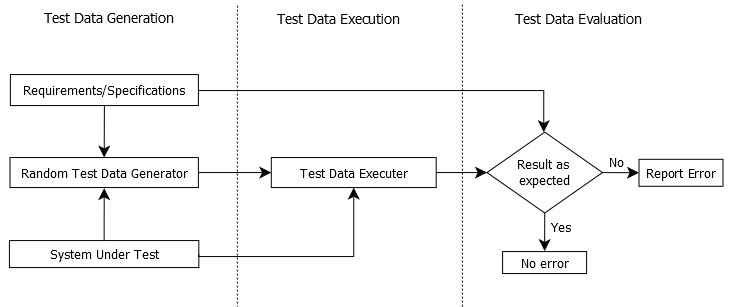
\includegraphics[width=15.3cm, height=8cm ]{chapter1/SoftwareTesting1.png}
		\bigskip
		\caption{Three main phases of random testing}
	\label{fig:SoftwareTesting1}
\end{figure}

This dissertation is a humble contribution to the literature on the subject, with the aim to bring about improvement in software testing by devising new, improved and effective automated software testing techniques based on random strategy.
\newpage
\section{The Problems}
Despite the benefits of random testing, its simplistic and non-systematic nature exposes it to high criticism~\cite{white1987software, myers2011art}. This research study focuses on the following problems in automated Random Testing (RT):
%Myers et al.~\cite{myers2011art} mentioned, ``probably the poorest methodology of all is random-input testing".  Despite the benefits of random testing, its simplistic and non-systematic nature exposes it to high criticism~\cite{white1987software}. Myers et al.~\cite{myers2011art} mentioned, ``probably the poorest methodology of all is random-input testing". However, Ciupa et al.~\cite{ciupa2008artoo} reported that the above stated statement of Myers et al. is based on intuition and lacks any experimental evidence. The criticism motivated the researchers to look into various aspects of random testing for evaluation and possible improvement. Adaptive random testing (ART)~\cite{chen2005adaptive}, Restricted Random Testing (RRT)~\cite{chan2006restricted}, Feedback Directed Random Testing (FDRT)~\cite{pacheco2007randoop}, Mirror Adaptive Random Testing (MART)~\cite{chen2004mirror} and Quasi Random Testing (QRT)~\cite{chen2007quasi} are a few of the enhanced random testing techniques reported in the literature.


\begin{enumerate}
\item Limitation of RT in the discovery of contagious failures.
\item Inability of RT to identify failure-domains.
\item Incompetence of RT to represent results in graphical form. 
\end{enumerate}

\subsection{Limitation of RT in the discovery of contagious failures}
Chan et al.~\cite{chan1996proportional} observed that failure inducing inputs are contagious and form certain geometrical patterns in the whole input domain. They divided them into point, block and strip patterns on the basis of their shape (Section~\ref{sec:artpatterns_2}). % put the failure domains section label in the preceeding reference.
The failure-finding ability of random testing technique decreases when the failures lie in contiguous block and strip patterns across the input domain.

\subsection{Inability of RT to identify failure-domains}
%As stated above, the failures in the input domain are contiguous and form point, block and strip patterns. 
The existing random strategies of software testing tries to discover failure individually and lack the capability to discover the failure domain.

%Random testing is also considered weak in providing high code coverage~\cite{cohen1997aetg, offutt1996semantic}. For example, in random testing when the conditional statement  ``$if (x == 25) then ... $"  is exposed to execution then there is only one chance, of the ``$then...$" part of the statement, to be executed out of $2^\text{32}$ available options. If $x$ is an integer variable of 32 bit value~\cite{godefroid2005dart}. 

\subsection{Incompetence of RT to represent results in a graphical form}
Random testing is no exception when it comes to the complexity of understanding and evaluating test results. Modern testing techniques simplify results by truncating the lengthy log files and displaying only the fault revealing test cases in the form of unit tests. No random strategy seems to provide graphical representation of the failures and failure-domains. Efforts are therefore required to get the test results of random testing in a user-friendly graphical form. 


\section{Research Goals}\label{ResearchGoals_1}
Goals of the research study are discovering how to leverage failure domain for finding more bugs and understanding the nature of failures and to develop new improved automated random test strategies to achieve the desired goals.

%The main goal of the research study is to develop new techniques for automated random testing with the aim to achieve the following objectives:

%\begin{enumerate}
%\item To develop a testing strategy with the capability to generate more fault-finding test data.

%\item To develop a testing technique for finding faults, fault domains and presentation of results on a graphical chart within the specified lower and upper bound. 

%\item To develop a testing framework with focus on increase in code coverage along with generation of more fault-finding test data. 

%\end{enumerate}

\section{Contributions}\label{contributions_1}
The main contributions of the thesis research are as follows: 

\subsection{Dirt Spot Sweeping Random Strategy}
%Development of a new enhanced and improved form of automated random testing: the Dirt Spot Sweeping Random (DSSR) strategy. This strategy is based on the assumption that faults and unique failures reside in contiguous blocks and stripes. The DSSR strategy starts as a regular random+ testing strategy � a random testing technique with preference for boundary values. When a failure is found, it increases the chances of using neighbouring values of the failure in subsequent tests, thus slowly sweeping values around the failures found in hope of finding failures of different kind in its vicinity.
%The DSSR strategy is implemented in the YETI random testing tool. It is evaluated against random (R) and random+ (R+) strategies by testing 60 classes (35,785 line of code) with one million ($10^\text{6}$) calls for each session, 30 times for each strategy. The results indicate that for 31 classes, all three strategies find the same unique failures. We analysed the 29 remaining classes using t-tests and found that for 7 classes DSSR is significantly better than both R+ and R, for 8 classes it performs similarly to R+ and is significantly better than R, and for 2 classes it performs similarly to random and is better than R+. In all other cases, DSSR, R+ and R do not perform significantly differently. Numerically, the DSSR strategy finds 43 more unique failures than R and 12 more unique failures than R+.

The failure-finding ability of the random testing technique decreases when the failures lie in contiguous locations across the input domain. To overcome the problem, a new automated technique: Dirt Spot Sweeping Random (DSSR) strategy was developed. It is based on the assumption that unique failures reside in contiguous blocks and strips. When a failure is identified, the DSSR strategy selects neighbouring values for the subsequent tests. The selected values sweep around the failure, leading to the discovery of new failures in the vicinity. Results presented in Chapter~\ref{chap:DSSR} indicate higher failure-finding ability of DSSR strategy as compared with Random (R) and Random+ (R+) strategies.

\subsection{Automated Discovery of Failure Domain}
The existing random strategies of software testing discover the faults in the SUT but lack the capability of presenting the fault domains. In the present study, a fully automated testing strategy named, ``Automated Discovery of Failure Domain (ADFD)" is developed with the ability to find the failures as well as the failure domains in a given SUT and provides visualisation of the identified pass and fail domains in a graphical form. The strategy implemented in YETI is described and practically illustrated by executing several programs of one and two dimensions in Chapter~\ref{chap:ADFD}. The experimental results prove that ADFD strategy automatically performs identification of failures and failure-domains and provides the results in graphical form.

\subsection{Automated Discovery of Failure Domain+ Strategy}
Another random test strategy named, ``Automated Discovery of Failure Domain+ Strategy'' (ADFD+) is developed in the current research study. 

%IGRS is an extended form of Random+ strategy guided by software invariants. Invariants from the given SUT are collected by Daikon, filtered by using DynComp and annotated in to source code as assertions. The IGRS is implemented in YETI and generates values in compliance with the added assertions. Experimental results presented in Chapter~\ref{chap:ADFD+} indicate improved features of IGRS in terms of higher code coverage and identification of subtle errors that R, R+ and DSSR strategies are either unable to accomplish or require larger duration.  

%\section{Structure of the Thesis}
%
%The rest of the thesis is organized as follows: In Chapter 2, a thorough review of the relevant literature is given. It includes a brief introduction of software testing techniques followed by automated random testing tools. Chapter~\ref{chap:DSSR} describes Dirt Spot Sweeping Random (DSSR) strategy, which is based on sweeping of fault clusters in the input domain. Chapter~\ref{chap:ADFD} presents the newly developed Automated Discovery of Fault Domains  (ADFD) strategy, which focuses on dynamically finding the faults and domains along with their graphical representation. Chapter~\ref{chap:IGR+S} presents the new strategy Invariant Guided Random+ Strategy (IGR+S) developed with the focus on quick identification of faults and increase in code coverage with the help of assertions. Chapter 6 summarizes contributions of the thesis research, discusses the strength and weaknesses of the study, gives conclusion and suggests avenues for future work. Chapter 7 ?



\section{Structure of the Thesis}
The rest of the thesis is organized as follows:\\

\hangindent=\parindent
\hangafter=1
\noindent
\textbf{Chapter~\ref{chap:softwareTesting}} provides literature review on software testing. Software testing is introduced with particular reference to its level, purpose, perspective and execution. Various types of software testing followed by major stages of testing including test data generation, execution, oracle and report production are reviewed with particular focus on literature relevant to random testing. Various versions of random testing and the most commonly used automated testing tools based on random algorithms are reviewed. \\


\hangindent=\parindent
\hangafter=1
\noindent
\textbf{Chapter~\ref{chap:yeti_3}} presents the York Extensible Testing Infrastructure (YETI), used as a tool in our experiments. YETI has been thoroughly reviewed including an overview, design, core infrastructure, strategy, language-specific binding, construction of test cases, command line options, execution, test oracle, report generation and graphical user interface.\\

\hangindent=\parindent
\hangafter=1
\noindent
\textbf{Chapter~\ref{chap:DSSR}} describes Dirt Spot Sweeping Random (DSSR) strategy. The proposed new testing technique is implemented in YETI. Experimental evidence is presented in support of the effectiveness of DSSR strategy in finding faults as compared with random and random+ strategies. 
% In majority of the classes DSSR strategy indicates higher fault-finding ability than random and random+ strategies. \\

\hangindent=\parindent
\hangafter=1
\noindent
\textbf{Chapter~\ref{chap:ADFD}} presents Automated Discovery of Failure Domain (ADFD) strategy. The proposed new testing technique, implemented in YETI, finds faults and fault domains in a specified limit and plots them on a chart. Experimental evidence is presented in support of ADFD strategy applied to several one and two dimensional programs. \\

 
\hangindent=\parindent
\hangafter=1
\noindent
\textbf{Chapter~\ref{chap:ADFD+}} presents the Automated Discovery of Failure Domain+ Strategy (ADFD+), a newly proposed testing technique that automatically generates invariants of SUT using Daikon, filter and annotate the invariants in the source code to better support testing process. The IGRS technique like DSSR and ADFD is also implemented in YETI. Experimental study is presented in which the effectiveness of IGRS in finding faults is compared with the random, random+ and DSSR strategies. 
% For the majority of the classes IGRS indicated higher fault-finding ability than the rival strategies.\\

\hangindent=\parindent
\hangafter=1
\noindent
\textbf{Chapter~\ref{chap:conclusion}} provides conclusion of the thesis \\

\hangindent=\parindent
\hangafter=1
\noindent
\textbf{Chapter~\ref{chap:futureWork}} gives proposals for future research in the relevant field. \\


 \hangindent=\parindent
 \hangafter=1
 \noindent
 \textbf{Appendix~\ref{chap:appendix1}} ADFD logic implementation and java programs with point, block and strip fault domain.\\

\newpage
\begin{figure}[h]
	\centering
		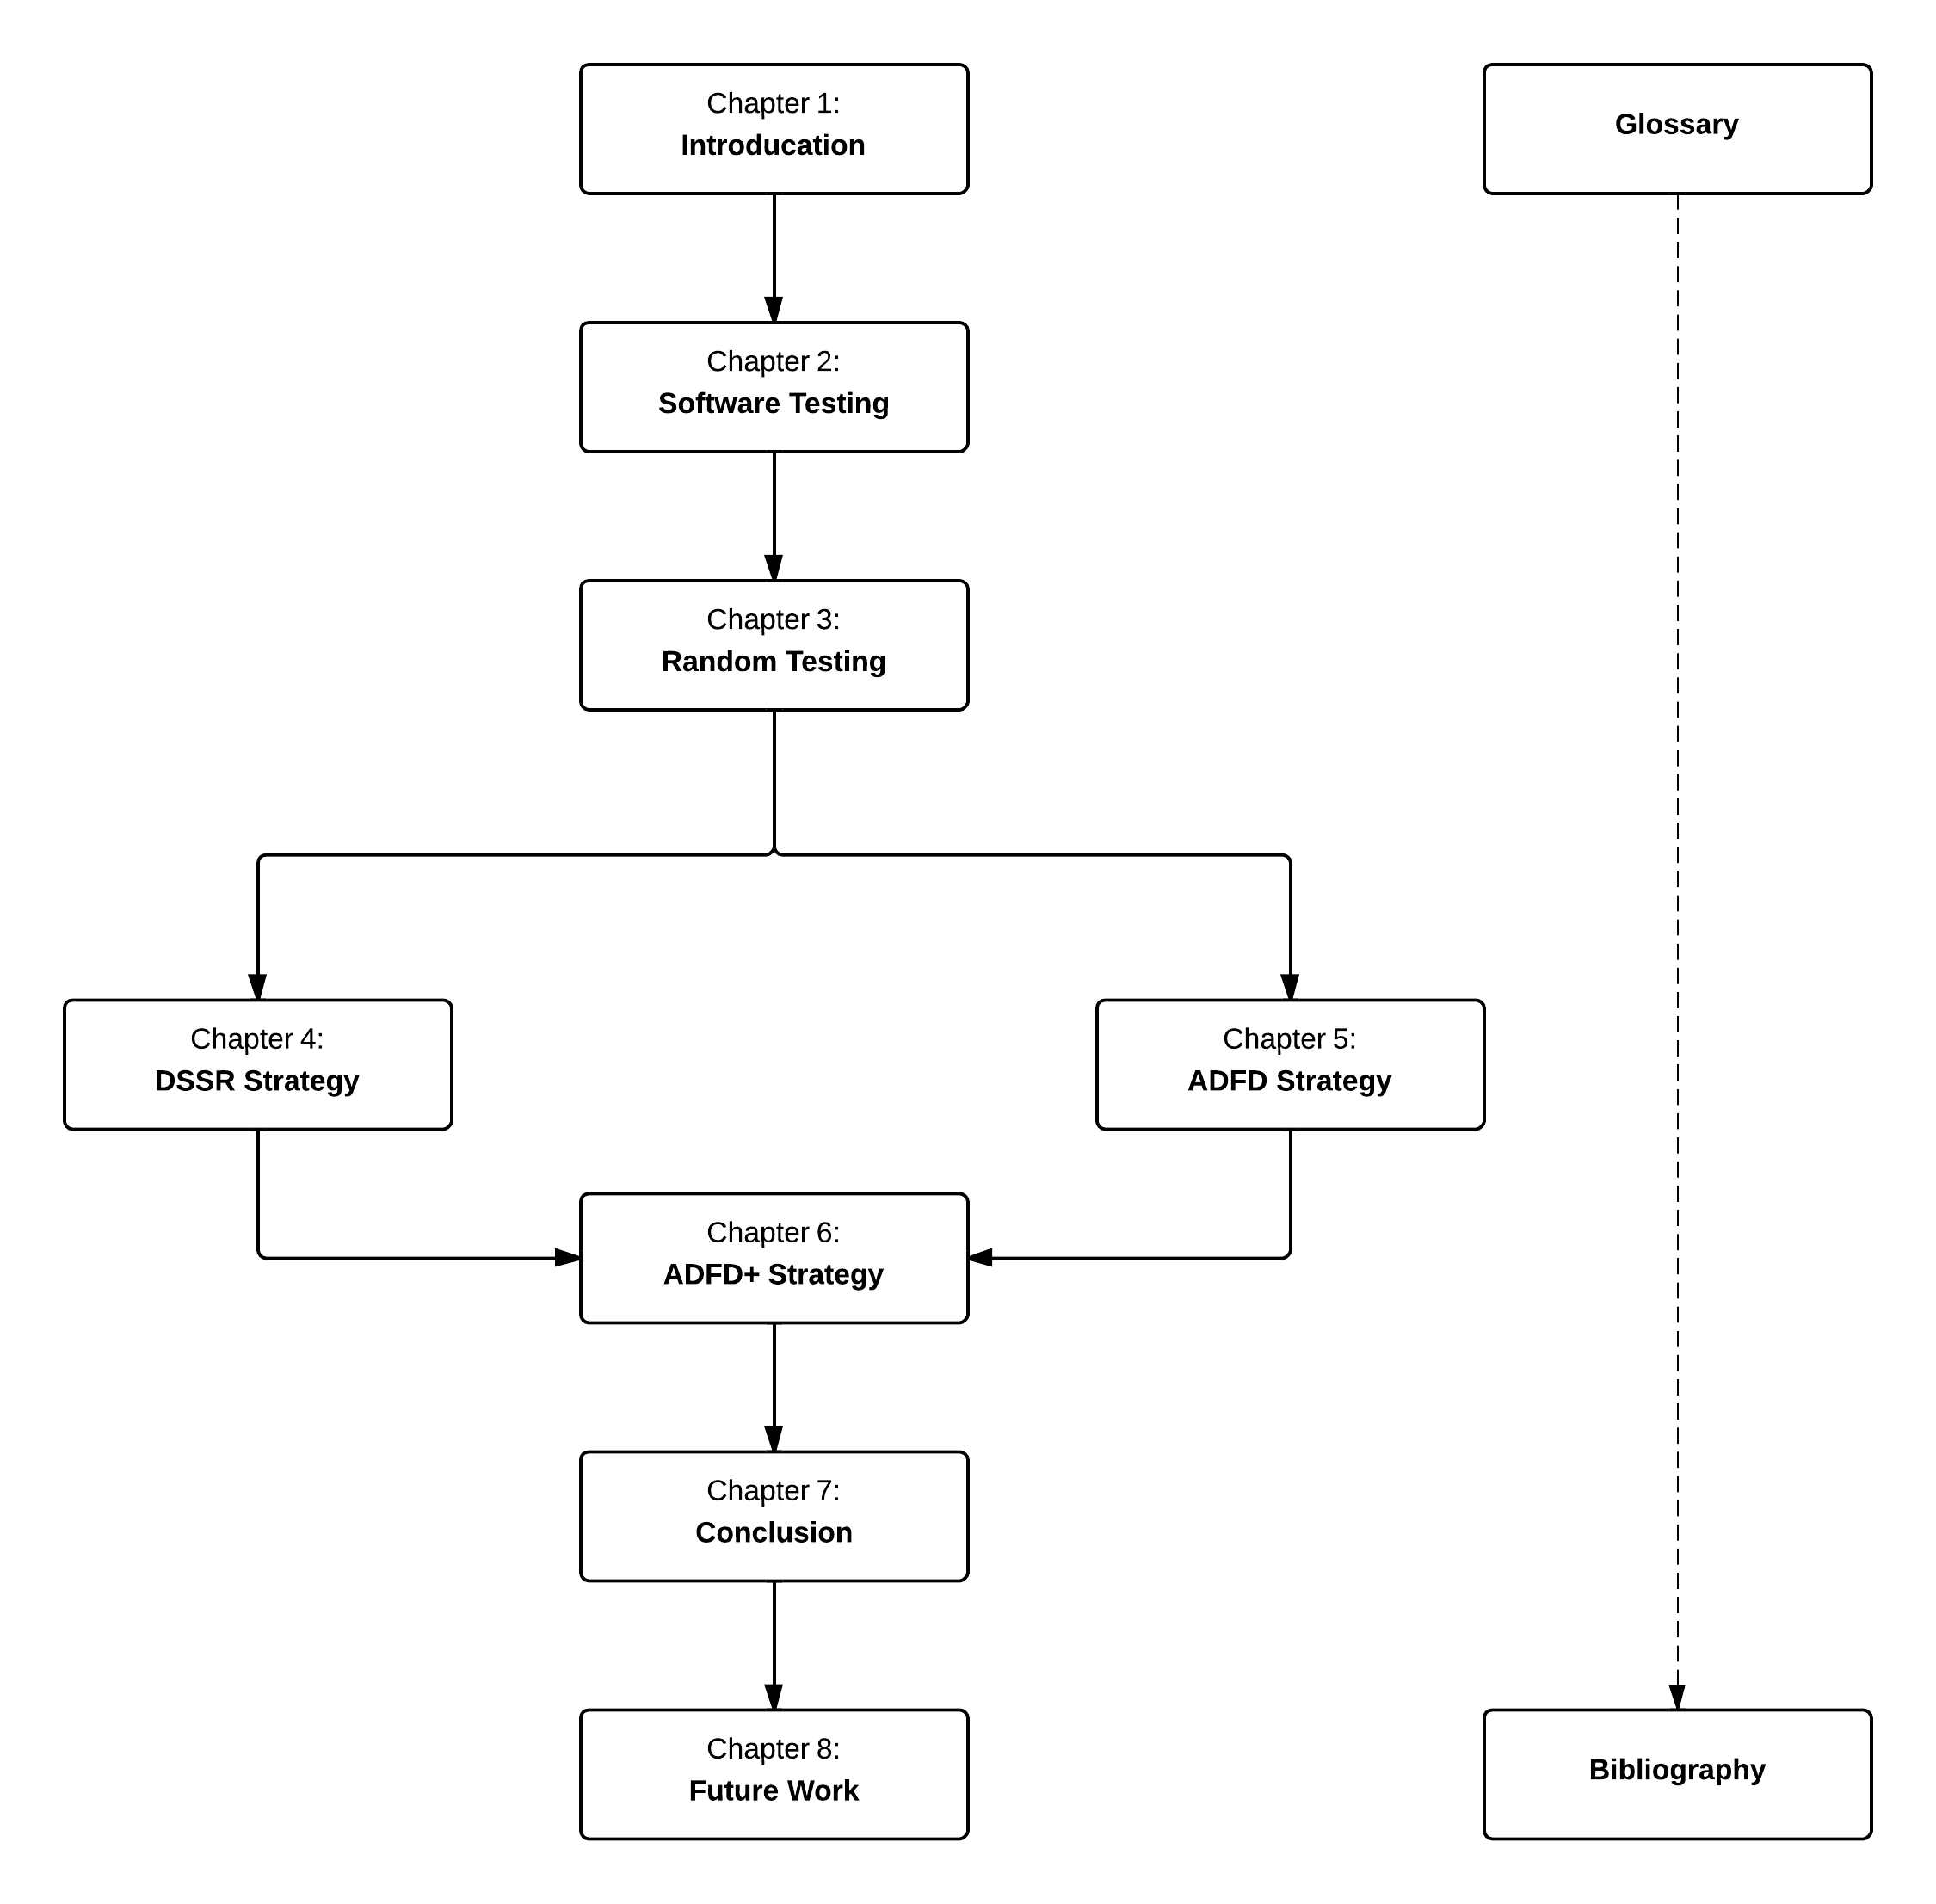
\includegraphics[width=16cm, height=20cm ]{chapter1/thesisOutline.png}
		\caption{Structure of thesis outline}
	\label{fig:thesisOutline}
\end{figure}



%Today, the primary focus of software companies is to achieve high quality. These companies spend an estimated thirty to ninety percent of the total software development cost on testing \ref{Beizer1990}, \ref{Standards2002}. In spite of spending 

%Software testing is the process of executing a software with specific test data followed by evaluation of the results to check whether it is working according to its specification or not \ref{Sommerville2006}.
% check here if we can replace specification with oracle or not.
%The test passes if the output complies to its specification and fails otherwise. The success of testing correlates with the number of failures found in the Software Under Test (SUT): a test is more successful if it finds more faults.

%It is interesting that program testing is used to show the presence of bugs, rather than absence of bugs [6]. Therefore the SUT that passes all the tests without returning a single failure does not guarantee that there is no fault. The testing process increases however the reliability and confidence of both the developers and the users in the tested product [7] [8] [9].

%Random testing is a black-box testing technique in which the SUT is executed against ran- domly selected test data. Test results obtained are compared either against the oracle defined, using SUT specifications in the form of assertions or exceptions defined by the programming language. The rapid increase in software development in today?s modern world prompts the need for automated testing to ensure high quality. The generation of random test data is com- paratively cheap and does not require too much intellectual and computation efforts [10] [11]. It is for this reason that various researchers have recommended this strategy for incorporation in automatic testing tools [12]. YETI [13] [14], AutoTest [15] [16], QuickCheck [17], Randoop [18], JArtage [19] are a few of the most common tools based on random strategy.


%%% ----------------------------------------------------------------------


%%% Local Variables: 
%%% mode: latex
%%% TeX-master: "../thesis"
%%% End: 

\chapter{Literature Review: Software Testing}
\label{chap:softwareTesting}
The very famous quote of Paul, ``to err is human, but to really foul things up you need a computer", is quite relevant to the software programmers. Programmers being humans are prone to errors. Therefore, in spite of best efforts, some errors may remain in the software after it is finalised.  Errors cannot be tolerated in software because a single error may cause a large upset in the system. The destruction of Mariner 1 rocket (1962) costing \$18.5 million was due to a small error in formula coded incorrectly by programmer. The Hartford Coliseum Collapse (1978) costing \$70 million, Wall Street crash (1987) costing \$500 billion, failing of long division by Pentium (1993) costing \$475 million, Ariane 5 Rocket disaster costing \$500 million were caused by minor errors in the software \cite{toweysoftware}. To achieve high quality, a software has to satisfy rigorous stages of testing. The more complex the software, the higher the requirements for software testing and the larger the damage caused when a bug remains in the software.

\begin{figure}[h]
	\centering
	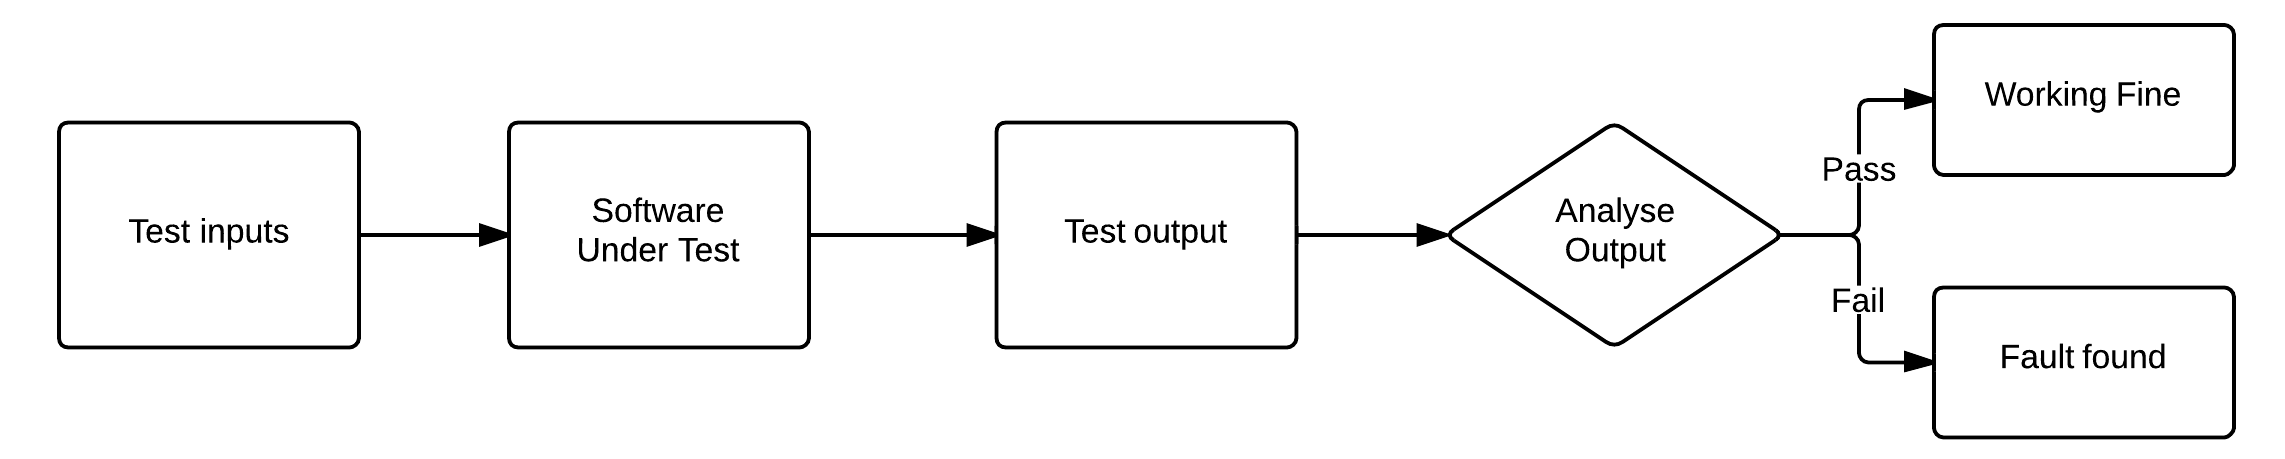
\includegraphics[width=15.5cm, height=4cm]{chapter2/softwareTesting.png}
	\caption{The process of software testing}
	\label{fig:softwareTesting}
\end{figure}

In the IEEE standard glossary of software engineering terminology~\cite{american1984}, testing is defined as ``the process of exercising or evaluating a system or system component by manual or automated means to verify that it satisfies the specified requirements and results". The process of software testing in its simplest form is shown in Figure~\ref{fig:softwareTesting}. 

The testing process, being an integral part of Software Development Life Cycle (SDLC), is started from requirement phase and continues throughout the life of the software. In traditional testing, when testers find fault in the given software, it is returned to the developers for rectification and consequently given back to the testers for retesting. It is important to note that a successful test is the one that fails a software or identifies fault in the software~\cite{Myers1979}. Fault denotes error made by programmers during software development~\cite{american1984}. A software that passes all the tests without giving a single error is not guaranteed to contain no error. The testing process, however, increases reliability and confidence of users in the tested product. \\


\begin{table}[ht]
%\scriptsize
\caption{Parts of Software Testing} % title of Table
\bigskip
\centering % used for centering table
{\renewcommand{\arraystretch}{1.5} %<- modify value to suit your needs
\begin{tabular}{| l | l | l | l | } % centered columns (4 columns)
\hline

Level 					&Purpose		 		& Perspective							& Execution 	\\
\hline
Unit						& Functional			& White Box							& Static 		\\
Integration				& Structural			& ~~~~~a. Data Flow Analysis				& Dynamic	\\
System					& Robustness			& ~~~~~b. Control Flow Analysis			&			\\
						& Stress				& ~~~~~c. Code-based fault injection &			\\
						& Compatibility			& Black Box							&			\\
						& Performance			& ~~~~~a. Use-case testing				&			\\
						&					& ~~~~~b. Partition testing				&			\\
						&					& ~~~~~c. Boundary Value testing			&			\\
						&					& ~~~~~d. Formal Specification testing		&			\\



\hline %inserts single line
\end{tabular}
}
\bigskip
\label{table:softwareTestingParts} % is used to refer this table in the text
\end{table}

\section{Definitions}
This section presents important definitions:

\subsection{Test Plan}
Test plan is a document which defines the goal, scope, method, resources and time schedule of testing \cite{futrell2001quality}. In addition, it includes the testable deliverables and the associated risk assessment. The test plan explains {\it {who, when, why}} and {\it {how}} to perform a specific activity in the testing process. 

\subsection{Input Domain} 
The input domain comprises of all possible inputs for a software, including all the global variables, method arguments and the externally assigned variables. For a given program P with input vector $ P =\{x1, x2, . . . , xn\}$, having $\{D1, D2, . . . , Dn\}$ as the domain of each input so that $x1 \in D1, x2 \in D2$ and so on, the domain D of a function is the cross product of the domains of each input: $D = D1 \times D2 \times . . . \times Dn$.

\subsection{Test Case}
%\begin{wrapfigure}{r}{0.35\textwidth}
%  \vspace{-20pt}
%  \begin{center}
%    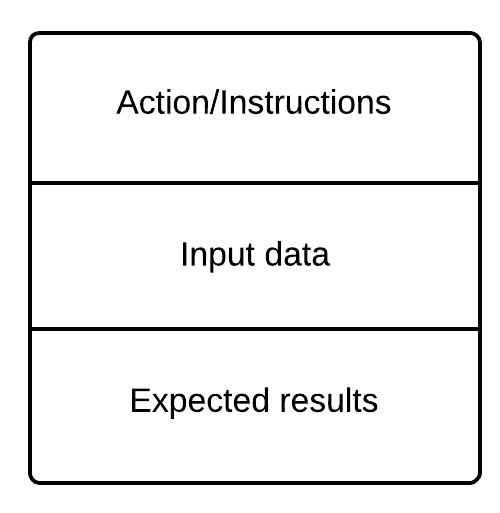
\includegraphics[width=0.30\textwidth]{chapter2/testCase.png}
%  \end{center}
%  \vspace{-20pt}
%  \caption{Test case}
%  \label{fig:testCase}
%  \vspace{-10pt}
%\end{wrapfigure}
A test case is an artifact which delineates the input, action and expected output corresponding to that input \cite{ahmed2010software}. After executing the test case, if the output obtained comply with the expected output, the test case is declared pass which means that the functionality is working correctly, otherwise the test case is declared fail, which represents identification of fault. A series of test cases, also known as test suite, are usually required to be executed for establishing the desired level of quality.

\section{Software Testing Levels}
Unit testing, Integration testing and System testing are the three main levels of software testing reported in the literature~\cite{chilenski1994applicability}. Unit testing deals with evaluation of code piece-by-piece and each piece is considered as independent unit. Units are combined together to form components. Integration testing is performed to make sure that integration of units in a component is working properly. Finally, system testing ensures that the system formed by the combination of components proceeds properly to give the required output.

\section{Software Testing Purpose}
The primary purpose of software testing is identification of faults in the given SUT for necessary correction in order to achieve high quality. Maximum number of faults can be identified if software is tested exhaustively. In exhausting testing SUT is checked against all possible combinations of input data and for assessment the results obtained are compared with the results expected. Exhaustive testing is not always possible in most scenarios because of limited resources and infinite number of input values that software can take. Therefore, the purpose of testing is generally directed to achieve confidence in the system involved from a specific point of view. For example, functionality testing is performed to check that functional aspect are working correctly. Structural testing analyses the code structure for generating test cases in order to evaluate paths of execution and identification of unreachable or dead code. In robustness testing the software behaviour is observed in the case when software receives input outside the expected input range. Stress and performance testing aims at testing the response of software under high load and checking its ability to process different nature of tasks~\cite{cohen2005robustness}. Finally, compatibility testing is performed to see the interaction of software with the underlying operating system.
 %As proper planning is the key to success for many projects this is often also true with software testing. A software test plan is a well defined document that defines the goal, scope, method, resources and time schedule of the testing.
%A software testing technique in which a software is tested with all possible combination of inputs. This technique can prove conclusively that the software meet its specification however exhaustive testing is seldom feasible because of the large input domain or too many paths in a software code. 

\section{Software Testing Perspective}
Software testing is divided into white-box and black-box testing based on the perspective taken.

\subsection{White-box testing}
In white-box or structural testing, the testers must know about the complete structure of the software so that they may make necessary modifications, if so required. Test cases are derived from the code structure and test passes only if the results are correct and the proper code is followed during test execution~\cite{ostrand2002white}. Some commonly used white-box testing techniques are as follows:
\begin{figure}[h]
\begin{center}
	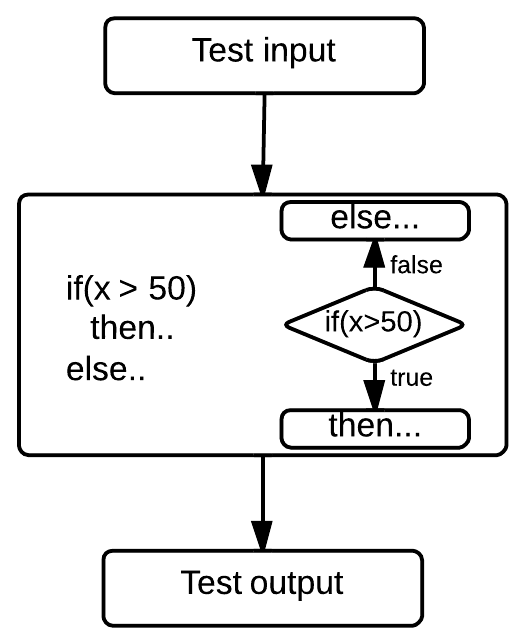
\includegraphics[width=5cm, height=6cm ]{chapter2/whiteBox.png}
	\caption{White-box testing}
	\label{fig:blackBox}
\end{center}  
\end{figure}
%\begin{wrapfigure}{r}{0.36\textwidth}
%  \vspace{-35pt}
%  \begin{center}
%   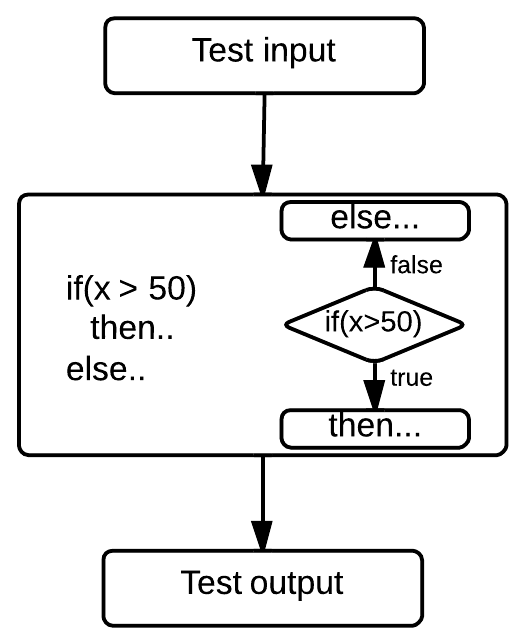
\includegraphics[width=0.30\textwidth]{chapter2/whiteBox.png}
%  \end{center}
%  \vspace{-20pt}
%  \bigskip
%  \caption{White-box testing}
%  
% \vspace{-18pt}
%\end{wrapfigure}

\subsubsection{Data Flow Analysis}
Data Flow Analysis (DFA) is a testing technique which focuses on the input values by observing the behaviour of respective variables during execution of the SUT~\cite{clarke1989formal}. In this technique a Control Flow Graph (CFG), graphically representing all possible states of a program, is drawn to determine the paths that are traversed by the program during test execution. Test cases are generated and executed to verify conformance with CFG. 

The process of program execution can be looked into as data-flow from input to output where data may transform into several intermediary steps before reaching the final state. The process is prone to several errors e.g. references made to non existing variables, values assigned to undeclared variables or change of variables in undesired manner. Ordered use of data is crucial to ensure that the aforementioned errors do not occur~\cite{fosdick1976data}.

\subsubsection{Control Flow Analysis}
Control Flow Analysis (CFA) is a testing technique which takes into consideration the control structure of a given SUT. Control structure is the order in which the statements, instructions or function calls are executed. In this technique a CFG, similar to the one required in DFA, is drawn to determine the traversable paths by a program during the execution. Test cases are generated and executed to verify conformance with CFG on the basis of control. Taking the example of following a specific path between two or more available choices at a particular state: efforts are made to ensure that, at least once, the set of selected test cases execute all the possible control choices. The effectiveness of the testing technique depends on measurement of control. Two of the most common measurement criteria defined by Vilkomir et al. are Branch coverage and Condition coverage~\cite{vilkomir2003tolerance}. 

\subsubsection{Code-based fault injection testing}
It is a testing technique in which new instructions are added to the code of the SUT at one or more locations to analyse the software behaviour in response to the instructions. \cite{voas1997software}. The process of code addition (instrumentation) is performed before compilation and execution of software. Code is added to: find error handling behaviour of software, examine the capability of test procedure and measure the code coverage achieved by the testing process.    

\subsection{Black-box testing}
In black-box or functional testing, the testers do not need to know about internal code structure of the SUT. Test cases are derived from the software specifications and test passes if the result is according to expected output~\cite{beizer1995black}. Some commonly used black-box testing techniques are stated below:
\begin{figure}[h]
\begin{center}
	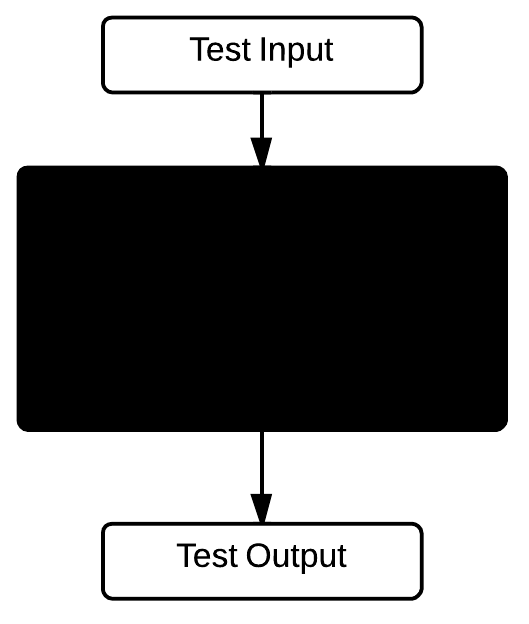
\includegraphics[width=5cm, height=6cm ]{chapter2/blackBox.png}
	\caption{Black-box testing}
 	\label{fig:blackBox}
\end{center}  
\end{figure}
%\begin{wrapfigure}{r}{0.35\textwidth}
%  \vspace{-35pt}
%  \begin{center}
%    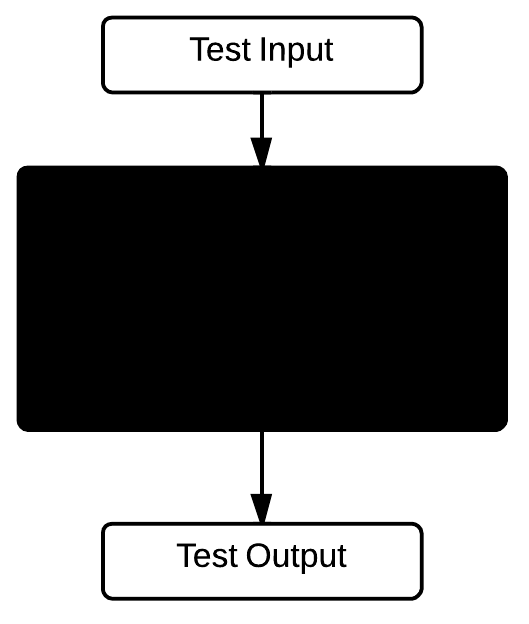
\includegraphics[width=0.30\textwidth]{chapter2/blackBox.png}
%  \end{center}
%  \vspace{-20pt}
%  \bigskip
%  \caption{Black-box testing}
%  \label{fig:blackBox}
%  \vspace{-18pt}
% \end{wrapfigure}
\subsubsection{Use-case based testing}
% check if it is use case-based testing or use case testing.
It is a testing technique which utilizes use-cases of the system to generate test cases. Use-case defines functional requirement at a particular point in the system from actor's perspective. It consists of a sequence of actions to represent a particular behaviour of the system. A use-case format includes brief description and flow of events, pre-conditions, post-conditions, extension points, context and activity diagrams. The use-case contains all the information required for test case, therefore, it can be easily transformed into a test case. Use-case testing is beneficial in terms of cheap generation of test cases, avoidance of test duplication, increased test coverage, easier regression testing and early identification of missing requirements.  

% steps taken from presentation of Raional User Conference 2003. Check it for viva.
\subsubsection{Partition Testing}
It is a testing technique in which the input domain of a given SUT is divided into sub-domains for testing each sub-domain individually. The division is based on software specifications, structure of the code and the process involved in software development~\cite{hamlet1990}. The performance of partition testing is directly dependant on the quality of sub-domain~\cite{weyuker1991analyzing}. However, division of input domain into equal partitions is often difficult. To overcome the problem, a new version of partition testing, called Proportional sampling strategy~\cite{Chan1996} is devised. In this version, the sub-domains vary in size and the number of test cases selected from each partition is directly proportional to the size of the partition. Experiments performed by Ntafos~\cite{ntafos1998random} has provided evidence for better performance of Proportional partition testing.


\subsubsection{Boundary Value Analysis}
Boundary Value Analysis (BVA) is a testing technique based on the assumption that errors often reside along the boundaries of the input variables. Thus border values are taken as the test data set in BVA. According to IEEE standards~\cite{radatz1990ieee}, boundary values contain minimum, maximum, internal and external values specified for a system. 

BVA  and partition testing may be used in combination by choosing test values from the whole input domain and also from the borders of each sub-domain. Reid et al. \cite{reid1997empirical} have provided evidence in support of better performance of BVA compared to partition testing. However, they have indicated that better performance of BVA is based on accurate identification of partition and selection of boundary values.

 The following code illustrates the ability of BVA to find a bug.  On passing interesting value \verb+MAX_INT+ as argument to the $test$ method, the code in the method increment it by 1 making it a negative value and thus an error is generated when the system try to build an array of negative size.

\begin{lstlisting}
~public void test (int arg) {
~~~~~arg = arg + 1;
~~~~~int [] intArray = new intArray[arg];
~~~~~...
~}
\end{lstlisting}



\subsubsection{Formal Specification Testing}
It is a testing technique based on mathematical model which provides the opportunity to handle the specifications mechanically. This feature facilitates the isolation, transformation, assembly and repackaging of the information available in the specifications for use as test cases~\cite{donat1997automating}.

The formal specification testing is more productive because of the creation of test cases independent from the code of the SUT~\cite{gaudel2010software}. The extra effort of generating test oracle is avoided because of using the available specification model for verifying the test results~\cite{bertolino2007software}.
  

%\section{Common Techniques of Software Testing}
%This section briefly define some of the most common techniques of software testing currently being used in the testing industry. These include techniques from both white-box and black-box testing techniques.

% Check wikipedia for them.


%\subsubsection{Grey-Box Testing}
%Grey-Box testing is the combination of both black-box/functionality and white-box/structural testing. The tester knows about both the functionality and the internal structure of the SUT. Some of the test cases are based on the functionality and some of the test cases are based on the structure. Emphasis of grey-box testing is both on code coverage as well as functionality~\cite{Savenkov2008}.

%\subsection{Software Testing Workflow}
%There are many software techniques like unit testing, integration testing, random testing, regression testing, system testing, acceptance testing, performance testing, load testing, stress testing, alpha testing, beta test etc. All testing techniques belong to black-box, white-box or grey-box approach. Each testing technique has its own strength and weaknesses but the technique in focus here is Random Testing.


%\begin{figure}[h]
%\begin{center}
%	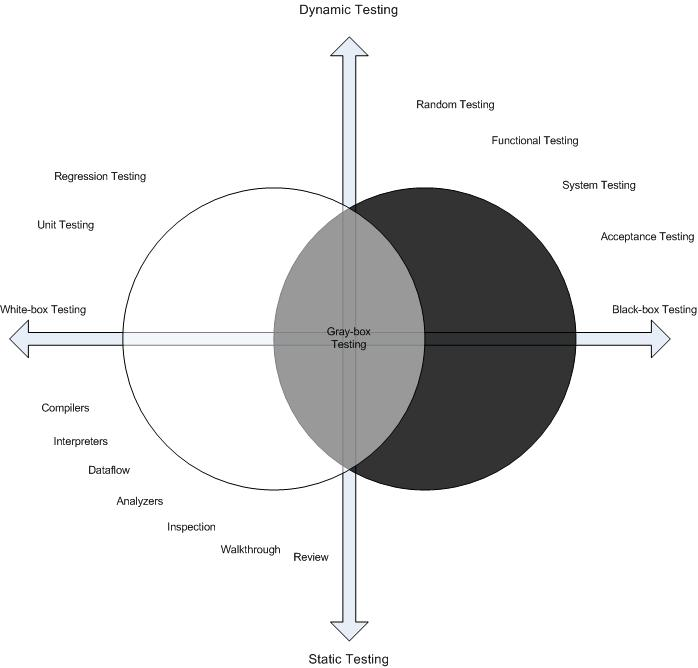
\includegraphics[width=16cm, height=12cm ]{Literature/Drawing34.jpg}
%	\caption{Software Testing Workflow}
%\end{center}  
%\end{figure}


%We have explained software testing graphically with the help of plotting venn diagram on two dimensional axis. The positive x axis represent black-box while negative x axis represent white-box testing. Grey-box testing in the middle is represented by the overlapping of black-box and white-box testing. Similarly on positive y axis we have dynamic testing and on negative y axis we have static testing.
%Now if a test is black box and dynamic then the test will fall in 0 to 90 degree on the diagram and if the test is black-box and static then it will fall in 270 to 360 degree. On the other hand if the test is white-box and dynamic then it will fall in 90 to 180 degree and if the test is white-box and static then it will fall in 180 to 270 degrees.

%\subsection{Automated Test Generation}
%\subsection{Generation Strategies}

\subsection{Test Oracle}
Test oracle is defined as, ``a source containing expected results for comparison with the actual result of the SUT" \cite{ahmed2010software}. For a program P, an oracle is a function which verifies that the output from P is the same as the output from a ‘correct’ version of P~\cite{howden1986}. Test oracle set the acceptable behaviour for test execution~\cite{baresi2001test}. 

All software testing techniques depend on the availability of test oracle~\cite{gaudel2010software}. Designing test oracle for ordinary software may be simple and straightforward. However, for relatively complex software, designing of oracle is quite cumbersome and requires special ways to overcome the oracle problem. Some of the common oracle problems are as follows:
\begin{enumerate}
\item It is assumed that the test results are observable and comparable with the oracle.
\item Ideally, test oracle would satisfy desirable properties of program specifications~\cite{baresi2001test}.
\item A test oracle to satisfy all conditions is seldom available as rightly pointed out by Weyuker, ``truly general test oracles are often unobtainable''~\cite{weyuker1982testing}. 
\end{enumerate}

Some common artefacts used as oracles are as follows.
\begin{enumerate}
\item Specification and documentation to generate test oracle. 
\item Products similar to the SUT but different in algorithm. %to solve the similar problem.
\item Heuristic algorithms to provide exact results for a set of test cases. % Hoffman, Douglas; Heuristic Test Oracles, Software Testing & Quality Engineering Magazine, 1999
\item Statistical characteristics to generate test oracle. % \cite{mayer2004test}. 
\item Comparison of the result of one test to another for consistency. % Hoffman, Douglas; Analysis of a Taxonomy for Test Oracles, Quality Week, 1998
\item Models to generate test oracle for verification of SUT behaviour. % \cite{robinson1999finite}.
\item Manual analysis by human experts to verify the test results. %\cite{jalote1997integrated}. 
\end{enumerate}

\section{Software Test Execution}
Software test execution can be either static or dynamic. In static testing test cases are analysed statically for checking errors without test execution. Besides code, high quality softwares are supplied with documentation including requirements, design, user manual, technical and marketing information. Reviews, walkthroughs or inspections are most commonly used techniques for static testing. In dynamic testing the software code is executed and input is converted into output. Results are analysed against expected outputs to find any error in the software. Unit testing, integration testing, system testing, and acceptance testing are most commonly used as dynamic testing methods~\cite{fairley1978tutorial}.

%Dynamic testing can be manual or automated. In manual testing the programmer develops the test cases which are executed by the developed software to find any error in processing or output. Similarly in automated testing the software or components of the software is given as input to testing software that automatically generates test cases and executes the SUT against them to find any errors. Manual testing typically consumes more time and resources than automated testing.



\subsection{Manual Software Testing}
Manual testing is the technique of finding faults in software in which the tester writes the code by hand to create test cases and test oracle~\cite{Ciupa2008}. Manual testing may be effective in some cases but it is generally laborious, time consuming and error-prone~\cite{tretmans1999}. Additionally, it requires that the testers must have appropriate skills, experience and knowledge of the SUT for evaluation from different perspectives.
 
\subsection{Automated Software Testing}
Automated testing is the technique of finding faults in a software in which a testing tool is used to perform the testing process automatically~\cite{Leitner2007}. There are tools which can automate part of a testing process e.g. generation of test cases or execution of test cases or evaluation of results. Other tools are available which can automate the whole testing process. The increase in functionality, productivity and lower cost of production without compromising quality are the desirable features in favour of automating the process of software testing. Automated software testing can be very effective and highly beneficial for any organisation. Its initial cost may be higher, however, a quick return on investment outperforms it and brings the key benefits of cost reduction, higher productivity, availability, reliability and performance. Automated testing is particularly effective when the nature of job is repetitive and is performed on routine basis like unit testing and regression testing, where the tests are re-executed after each modification \cite{huang2003automated}. The use of automated software testing made it possible to test large volumes of code, which would have been impossible otherwise~\cite{ramamoorthy1975testing}.

\section{Test Data Generation}
Test data generation in software testing is the process of identifying test input data which satisfies the given test selection criterion. A test data generator is used to assist testers in the generation of test data while the test selection criterion define the properties of test cases to be generated based on the test plan and perspective taken \cite{korel1990}. Various artefacts of the SUT can be considered to generate test data like requirements, model, code etc. The choice of artefacts selected limits the kind of test selection criteria that can be applied in guiding the test case generation. 

A typical test data generator consists of three parts: Program analyser, Strategy Handler and Generator \cite{edvardsson1999survey}. Program analyser performs initial assessment of software prior to testing and may alter the code if so required. For example it performs code instrumentation or construction of CFG to measure the code coverage during testing. A strategy handler define the test case selection criteria. This may include the formalisation of test coverage criterion, the selection of paths, normalisation of constraints, etc. It may also get input from   program analyser or user before or during execution. The generator taking inputs from the program analyser and strategy handler generates test cases according to the set selection criteria.  Test data generators based on their approaches are classified into path-wise, goal-oriented, intelligent and random test. Each type is briefly described in the following section.

\subsection{Path-wise Test Data Generator}
It is a technique in which the test data is generated to target path, statement and branch coverage in a given SUT. The approach generally consists of three main parts: CFG construction, path selection and test data generation. 

In path-wise test data generation, the program path to the selected statement is identified and the input data are generated for evaluating the path which can be either generated automatically or provided by the user. The data generated in path testing expresses boolean behaviour i.e. true or false for a particular node in a path. 

A complete path contains multiple sub-domains, each sub-domain consists of test inputs required to traverse the path. The boundary of the sub-domains are obtained by the predicates in the path condition. The test data traversing a certain path in the software are selected from an input space split into a set of sub-sections. 

% the pathwise test data generation is taken from a book knowldge mining using intelligent systems. you can reference it too.


\subsection{Goal-oriented Test Data Generators}
It is a technique in which the test data is generated to target a specific program point rather than a program path \cite{chungautomated}. The tester can select any path among a set of existing paths as long as it reaches to the specified program point. This technique utilizes runtime information for computing accurate test data~\cite{ferguson1996chaining}. Among various methods used in goal-oriented test data generation the following two commonly adopted approaches are briefly described.

\subsubsection{Chaining Approach}
The chaining approach uses data dependent analysis to guide the test data generation. In the process all the related statement are selected automatically by the technique that are affected by the execution of the selected statement under test. The dependant statements are executed before the selected statement to generate the required necessary data for the execution of the statement under test~\cite{ferguson1996chaining}.

The chaining approach analyses the program according to the edges and nodes. For each test coverage criterion different initial event sequence and goal nodes are determined. For example, consider  the branch (p, q), where p is  the starting node of the branch and q is the last node in the branch. The initial event sequence E for the branch (p, q) is defined as $E =< (s,\phi), (p,\phi),(q,\phi) >$, provided that s is the starting node of the program and $\phi$ is the set of variables referred to as a constraint. The the Branch Classification process identifies critical, semi-critical and non-critical nodes for each branch. During the execution of the program, this classification leads the search to decide which branch to take to reach the goal node or to cover the specified branch.  


\subsubsection{Assertion-oriented Approach}
In this approach assertions are added to the program code with the goal to identify program input on which an assertion is violated, indicating a fault in the SUT. An assertion specifies a constraint that applies to some state of a computation which evaluates to either true or false. For example, consider a given assertion A, now find program input x on which assertion A is false, i.e. when the program is executed on input x and the execution reaches assertion A. It is evaluated as false indicating a fault in the SUT.

It is not always possible to generate test cases that violate assertions. However, experiments have shown that assertion-oriented test data generation may frequently detect errors in the program related to assertion violation. The major advantage of this approach is that each generated test data uncovers an error in the program with violation of an assertion. An assertion is violated because of three reasons: a faulty, a faulty assertion and a faulty precondition.

% check the korel1996assertion for the above whole text and assertion oriented approach + the model hard copy thesis.


\subsection{Intelligent Test Data Generators}
 Intelligent test data generation is a technique used to overcome the problems associated with traditional data generation techniques like generation of meaningless data, duplicated data and failing to generate complex test data. The approach increases users confidence in the generated test data and the testing process~\cite{ramamoorthy1975testing}. It performs sophisticated analysis, such as fuzzy logic, neural networks and genetic algorithms on the SUT to assist in finding the appropriate test data. It involves complex analysis to anticipate different situations that may arise at any point. The approach produces test data which satisfy the SUT requirements, however, it consumes more time and resources.

\subsubsection{Genetic Algorithm}
Genetic algorithm is a heuristic that mimics the evolution of natural species in searching for the optimal solution of a problem. The solution sought by the genetic algorithm is the test data that causes execution of a given statement, branch, path and condition in the SUT. The genetic algorithm is guided by control dependencies in the program to search for test data which satisfy test requirements. The genetic algorithm constructs new test data from previously generated test data. The algorithm evaluates the existing test data, and guide the direction of search by using the programs control-dependence graph \cite{pargas1999test}.

The benefit of the genetic approach is quick generation of test data with focus and direction. New test cases are generated by applying simple operations on existing test cases that are judged to have good potential of satisfying the test requirements. The success of this approach, however, depends heavily on the way in which the existing test data is measured \cite{pargas1999test}.

% Please paraphrase the above section genetic algorithm.

\subsection{Random Test Data Generators}

Random test data generator is the simplest technique for generation of test data. It has the advantage of being used to generate input data for any type of program. However, random test data generation is based solely on probability and cannot accomplish high coverage as its chances of finding semantically small faults are quite low [3find that reference].

If a fault is only revealed by a small percentage of the program input it is said to be a semantically small fault. For example of a semantically small fault consider the following code:
\begin{lstlisting}
void test(char x,char y) {
    if (x==y)
        System.out.println("Equal");
    else
        System.out.println("Not Equal");
}
\end{lstlisting}

It is easy to see that the probability of execution of the first statement is significantly lower than that of the second statement. As the structure gets complex so does the probability of its execution. Thus, such semantically small faults are hard to find by using random test data generation. 

\subsection{Search-based Test Data Generation}
It is a technique that uses meta-heuristic algorithms to guide generation of test data. In Search-based test data generation technique each input vector x can be associated with a measure $cost(x)$ that represents how far away the input vector x is from satisfying the set goal. Input test values closer to the set goal have low cost values and the other have high cost values. 

Consider a program with an initial branch statement: ${\it{ if (x >= 20) y = z; else y = 2 * z;}}$ and suppose we want the true branch to be executed. An input value of $x == 25$ clearly satisfies the predicate, and a value of $x == 15$ can be seen to come closer to satisfying the predicate than a value of $x ==5$. We might evaluate a cost function probe ( immediately before the indicated statement) of the form $cost(x) = max {0, 20 - x}$. Thus $x == 25$ has cost $0$, $x == 15$ has cost $5$ and $x = 5$ has cost $15$. We can see how finding data to satisfy the branch predicate is essentially a search over the input domain of x to find a value such that $cost(x) == 0$. 

Similarly, finding data to follow a particular path in the code can be considered as the one which satisfy each of the number of predicate at different points. This leads to a cost function which combines the costs at each of the relevant branching points. The approach requires the measurement of state at appropriate points in a programs execution. Moreover, the cost function plays the role of oracle for each targeted test requirement. Consequently, the cost function must change as per requirement. Frequent re-instrumentation of program is required to find test data that fully satisfy common coverage criteria. 

%At its heart search based software testing requires the use of search or optimisation algorithms. Most standard heuristic search techniques have been used, e.g. hill-climbing, simulated annealing, tabu search and genetic algorithms. 

% The details need not concern us here, and the reader is referred to McMinn [50] for details. Overall the search based 





%\subsection{Using A Model Checker}
%\subsection{Test Case Generation with Gatel by Using Lustre}
%\subsection{Using Models in Z}
%\subsectioin{Using UML Diagrams}
%\subsection{Using Misuse / Abuse Cases for Robustness Testing}
%\subsection{Randomly-generated test suites} % Dynamically discovering likely program invariants thesis page 77
%\subsection{Grammar-generated test suites Randomly}% Dynamically discovering likely program invariants thesis page 78
%\subsection{Test-case generation} %Combining over-and under-approximating program analysis for automatic software testing (section 4.2)
%\subsection{Mutation generation} % Automatic testing of software with structurally complex inputs. page 79 section 7.2.1
%\subsection{Test Data Generation} % page 70, 4.6.1, Coverage analysis for GUI Testing
% Check Generating Structurally complex tests from declarative constraints thesis 




% add diagram for generators similar to john paper in automated program flaw finding using simulated annealing.








%\section{Automated Random Testing}
%\subsection{Test Data Generation}
%\subsection{Test Execution}



%\subsection{Test Report}

\section{Summary}
The chapter gives an overview of software testing process, starting from defining what software testing is, why it is necessary, its common types and the purpose for which they are used. It then differentiate between manual and automated software testing and finally various ways of software test data generation, being the most critical and crucial part of any testing system are studied.


% ------------------------------------------------------------------------


%%% Local Variables:
%%% mode: latex
%%% TeX-master: "../thesis"
%%% End:

\chapter{Literature Review: Random Testing}
\label{chap:randomTesting}

%\section{Random Testing}

Random testing was first mentioned in the literature by Hanford in 1970. He reported syntax machine, a tool that randomly generated data for testing PL/I compilers~\cite{hanford1970automatic}. Later in 1983, Bird and Munoz described a technique to produce randomly generated and self checking test cases~\cite{bird1983automatic}. 

%Work on random test generation dates back to a 1970 paper by Hanford. In it he reports on the ``syntax machine", a program that generated random but syntactically-correct programs for testing PL/I compilers \cite{hanford1970automatic}. The next published work on random testing was a 1983 paper by Bird and Munoz \cite{bird1983automatic}. They describe a technique to generate randomly-generated ``self-checking" test cases: test cases that in addition to generating test inputs generated checks for expected outputs using knowledge of the semantics of the software under test. For example, when generating random programs for testing a compiler, the generator kept track of the expected values of arithmetic computations and inserted the appropriate checks into the test case. They also applied their technique to checking sorting and merging procedures and graphic display software~\cite{pacheco2009directed}.

%One of the best-known works in the field is Miller et al.’s “fuzz testing” paper, where they generate random ASCII character streams and use them as input to test Unix utilities for abnormal termination or non-terminating behaviour \cite{miller1990empirical}. In subsequent work, they extended fuzz testing to generate sequences of keyboard and mouse events, and found errors in applications running in X Windows, Windows NT and Mac OS X \cite{forrester2000empirical, miller2006empirical}. Today, fuzz testing is used routinely in industry. It is frequently used as a tool for finding security vulnerabilities and is applied to test formats and protocols that attackers might use to gain unauthorized access to computers over a network. Other work that applies random test generation to operating systems code includes Kropp’s use of random test generation to test low-level system calls \cite{kropp1998automated}, and Groce et al.’s use of random test generation at NASA to test a file system used in space missions \cite{groce2007randomized}. In all these studies, a random test generator invariable found many errors in the software under test, and many errors were critical in nature. For example, Groce et al. found dozens of errors in the file system under test, many of which could have jeopardized the success of a mission.

Random testing is a dynamic black-box testing technique in which the software is tested with non-correlated unpredictable test data from the specified input domain~\cite{Chan2002}. As stated by Richard~\cite{hamlet1994}, in random testing, input domain is first identified, then test data are randomly taken from it by means of random generator. The program under test is executed on the test data and the results obtained are compared with the program specifications. The test fails if the results are not according to the specifications and vice versa. Fail results of the test cases reflects failure in the SUT.

\begin{figure}[h]
	\centering
	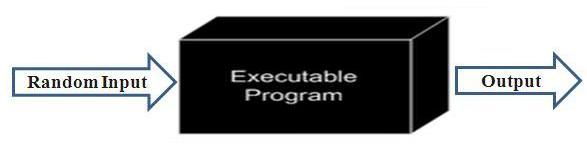
\includegraphics[width=13cm, height=3.5cm ]{chapter3/randomTesting.jpg}
	\caption{Random Testing}
\end{figure}

Generating test data by random generator is quite economical and requires less intellectual and computational efforts~\cite{Ciupa2008a}. Moreover, no human intervention is involved in data generation which ensures an unbiased testing process. However, generating test cases with out using any background information makes random testing susceptible to criticism. Random testing is criticized for generating many of the test cases that falls at the same state of software. It is also stated that, random testing generates test inputs that violates requirements of the given SUT making it less effective~\cite{pacheco2009directed, sen2007effective}. Myers mentioned random testing as one of the least effective testing technique~\cite{Myers1979}. However, Ciupa et al. stated~\cite{Ciupa2007}, that Myers statement was not based on any experimental evidence. Later experiments performed by several researchers~\cite{Ciupa2008, hamlet1994,  leitner2007efficient, Duran1981} confirmed that random testing is as effective as any other testing technique. It is reported~\cite{Duran1981} that random testing can also discover subtle faults in a given SUT when subjected to large number of test cases. It is pointed out that the simplicity and cost effectiveness of random testing makes it more feasible to run large number of test cases as opposed to systematic testing techniques which require considerable time and resources for test case generation and execution. The empirical comparison proves that random testing and partition testing are equally effective~\cite{hamlet1990}. A comparative study conducted by Ntafos~\cite{ntafos1998random} concluded that random testing is more effective as compared to proportional partition testing. A prominent work to mention is that of Miller et al.~\cite{miller1990empirical}, who generated and used random ASCII character streams to test Unix utilities for abnormal termination or non-terminating behaviour. Subsequently the same technique was extended to discover errors in softwares running on X Windows, Windows NT and Mac OS X \cite{forrester2000empirical, miller2006empirical}. Other famous studies using random testing includes low-level system calls \cite{kropp1998automated}, and file systems used in missions at NASA \cite{groce2007randomized}.


\section{Various versions of random testing}
Researchers have tried various approaches to bring about improved versions of random testing with better performance. The prominent versions of random testing are as follows:

\subsection{Adaptive Random Testing}
Adaptive random testing (ART), proposed by Chen et al.~\cite{Chen2008} is based on the previous work of Chan et al.~\cite{Chan1996} regarding the existence of failure patterns across the input domain. Chan et al. observed that failure inducing inputs formed certain geometrical patterns in the whole input domain which were divided into point, block and strip patterns described below.

\begin{enumerate}
\item {\bf Point pattern:} In the point pattern, inputs inducing failures are scattered across the input domain in the form of stand-alone points. Example of point pattern is the division by zero in the statement: $total = num1/num2;$ where $num1$, $num2$ and $total$ are variables of type integer.
\item {\bf Block pattern:} In the block pattern, inputs inducing failures lie in close vicinity to form a block in the input domain. Example of block pattern is failure caused by the statement: $if ( (num \textgreater 10) \&\& (num \textless 20) )$. Here 11 to 19 are a block of faults.
\item {\bf Strip pattern:} In the strip pattern, inputs inducing failures form a strip across the input domain. Example of strip pattern is failure caused by the statement: $num1 + num2 = 20$. Here multiple values of $num1$ and $num2$ can lead to the fault value 20. 
\end{enumerate}

\begin{figure}[h]
	\centering
	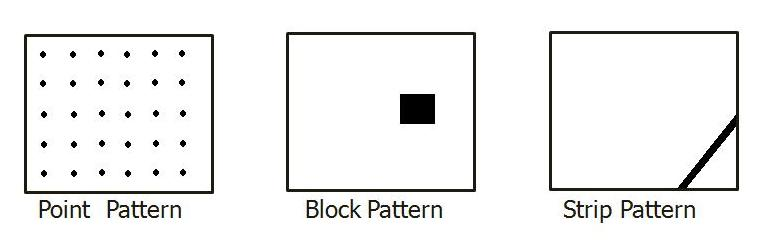
\includegraphics[width=13cm, height=5.7cm ]{chapter3/pointblockstrip.jpg}
	\caption{Patterns of failure causing inputs~\cite{Chan1996}}
	\label{fig:patterns2}
\end{figure}

In Figure~\ref{fig:patterns2} the three square boxes indicate the whole input domains. The white space in each box shows legitimate and faultless values while the black colour in the form of points, block and strip, inside the respective boxes indicates the faults in the form of point, block and strip patterns.

Chen et al.~\cite{Chen2008} argued that ordinary random testing might generate test inputs lurking too close or too far from the input inducing failure and thus fails to discover the fault. To generate more fault-targeted test inputs, they proposed Adaptive Random Testing (ART) as a modified version of random testing where test values are selected at random as usual but are evenly spread across the input domain by using two sets. The executed set comprises the test cases and the candidate set includes the test cases to be executed by the system. Initially both the sets are empty. The first test case is selected at random from the candidate set and stored in executed set after execution. The second test case is then selected from the candidate set which is far away from the last executed test case. In this way the whole input domain is tested with greater chances of generating test input from the existing fault patterns.

In the experiments conducted by Chen et al.~\cite{Chen2008}, the number of test cases required to detect first fault (F-measure) was used as a performance matrix instead of the traditional matrices (P-measure) and (E-measure). Experimental results using ART showed up to 50\% increase in performance compared to random testing. The authors pointed out that the issues of increase overhead, spreading test cases across the input domain for complex objects and efficient ways of selecting candidate test cases still exist. Chen et al. continued their work on ART to address some of these issues and proposed its upgraded versions~\cite{Chen2005, chen2009enhanced}. 

\subsection{Mirror Adaptive Random Testing}
%As discussed in the above section ART provide better results, however the increase in overhead due to extra computation to achieve even spread of test inputs makes it less cost effective. 
Mirror Adaptive Random Testing (MART)~\cite{Chen2003} is an improvement on ART by using mirror-partitioning technique to reduce the overhead by decreasing the extra computation involved in ART. 

\begin{figure}[h]
\begin{center}
	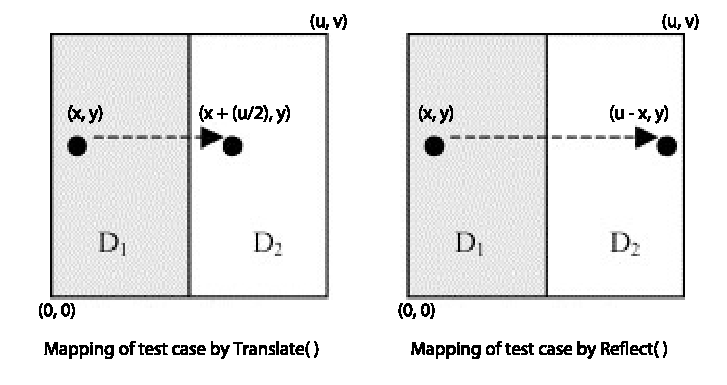
\includegraphics[width=13.5cm, height=6.5cm ]{chapter3/mart2.pdf}
	\caption{Mirror Adaptive Random Testing~\cite{Chen2003}}
\label{fig:mirrorART}
\end{center}  
\end{figure}

In this technique, the input domain of the program under test is divided into n disjoint sub-domains of equal size and shape. One of the sub-domains is called source sub-domain while all others are termed as mirror sub-domains. ART is then applied only to the source sub-domain while test cases are selected from all other sub-domains by using mirror function. In MART $(0, 0), (u, v)$ are used to represent the whole input domain where $(0, 0)$ is the leftmost and $(u, v)$ is the rightmost top corner of the two dimensional rectangle. On splitting it into two sub-domains we get {(0, 0), (u/2, v)} as source sub-domain and $(u/2, 0), (u, v)$ as mirror sub-domain. Suppose we get $x$ and $y$ test cases by applying ART to source sub-domain, now we can linearly translate these test cases to achieve the mirrored effect, i.e. $(x + (u/2), y)$ as shown in the Figure~\ref{fig:mirrorART}. 

Comparative study of MART with ART provide evidence of equally good results of the two strategies with MART having the added advantage of lower overhead by using only one quarter of the calculation as compared with ART.


\subsection{Restricted Random Testing}
Restricted Random Testing~\cite{chan2003normalized} is another approach to overcome the problem of extra overhead in ART. Restricted Random Testing (RRT) achieves this by creating a circular exclusion zone around the executed test case. A candidate is randomly selected from the input domain for the next test case. Before execution the candidate is checked and discarded if it lies inside the exclusion zone. This process repeats until a candidate laying outside the exclusion zone is selected. This ensures that the test case to be executed is well apart from the last executed test case. The radius of exclusion zone is constant in each test case and the area of input domain decreases progressively with successive execution of test cases.

\begin{figure}[h]
	\centering
	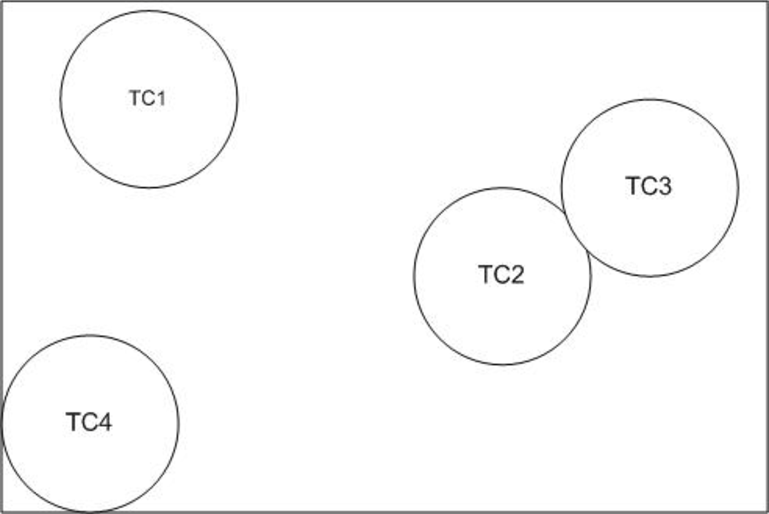
\includegraphics[width= 8cm, height = 6.5cm]{chapter3/RRT.pdf}
	\caption{Input domain with exclusion zone around the selected test case}
\end{figure}

The above authors compared RRT with ART and RT to find the comparative performance and reported that the performance of RRT increases with the increase in the size of the exclusion zone and reaches the maximum level when the exclusion zone is raised to largest possible size. %Normalized Restricted Random Testing~\cite{chan2003normalized} is an improvement over RRT by allowing the testers to have better information about the target exclusion rate (R) of RRT. 
They further found that RRT is up to 55\% more effective than random testing in terms of F-measure.



\subsection{Directed Automated Random Testing}
Godefroid et al.~\cite{Godefroid2005} proposed Directed Automated Random Testing (DART). %Its main purpose was to overcome the cost and difficulty of manual testing while keeping its quality intact. It automate the whole testing process including generation of unit tests, test drivers/harness and assertions for functional correctness. 
The following main features of DART are reported in the literature:
\begin{enumerate}
\item {\bf Automated Interface Extraction:} DART automatically identifies external interfaces of a given SUT. These interfaces include external variables and methods and the user-specified main method responsible for program execution.
\item {\bf Automatic Test Driver:} DART automatically generate test drivers for running the test cases. All the test cases are randomly generated according to the underlying environment.
\item {\bf Dynamic Analysis of execution:} DART instrument the given SUT at the start of the process in order to track its behaviour dynamically at run time. The results obtained are analysed in real time to systematically direct the test case execution along alternative path for maximum code coverage.
\end{enumerate}

The DART algorithm is implemented in the tool which is completely automatic and accepts the test program as input. After the external interfaces are extracted it then use the pre-conditions and post-conditions of the program under test to validate the test inputs. For languages that do not support contracts inside the code (like C), they used public methods or interfaces to mimic the scenario -------- to be continued

\subsection{Quasi Random Testing}
Quasi-random testing (QRT)~\cite{Chen2005} is a testing technique which takes advantage of failure region contiguity for distributing test cases evenly and thus decreases computation. %Chan et al after the analysis of faults in various experiments found that the fault patterns across the input domain are continuous. 
To achieve even spreading of test cases, QRT uses a class with a formula that forms an s-dimensional cube in s-dimensional input domain and generates a set of numbers with small discrepancy and low dispersion. The set of numbers is then used to generate random test cases that are permuted to make them less clustered and more evenly distributed. An empirical study was conducted to compare the effectiveness of QRT with ART and RT. The results showed that in 9 out of 12 programs QRT found a fault quicker than ART and RT while there was no significant improvement in the remaining three programs.
%\subsection{Monti Carlo Random Testing}

%\subsection{Good Random Testing}

\subsection{Feedback-directed Random Testing}
Feedback-directed Random Testing (FDRT) is a technique that generates unit test suite at random for object-oriented programs~\cite{Pacheco2007}. As the name implies FDRT uses the feedback received from the execution of first batch of randomly selected unit test suite to generate next batch of directed unit test suite. In this way redundant  and wrong unit tests are eliminated incrementally from the test suite with the help of filtration and application of contracts. For example unit test that produce IllegalArgumentException on execution is discarded, because, selected argument used in this test is not according to the type of argument the method required. 

%\subsection{Adaptive Random Testing for Object-Oriented}
\subsection{The ARTOO Testing}
The Adaptive Random Testing for Object Oriented (ARTOO) strategy is based on object distance. Ciupa et al.~\cite{Ciupa2006} defined the parameters that can be used to calculate distance between the objects. Two objects have more distance between them if they have more dissimilar properties. The parameters to specify the distance between the objects are dynamic types and values are assigned to the primitive and reference fields. Strings are treated in terms of directly usable values and Levenshtein formula~\cite{Levenshtein1966} is used as a distance criterion between the two strings.

In the ARTOO strategy, two sets are taken i.e. candidate-set containing the objects ready to be run by the system and the used-set, which is empty. First object is selected randomly from the candidate-set which is moved to used-set after execution. The second object selected from the candidate-set for execution is the one with the largest distance from the last executed object present in the used-set. The process continues till the bug is found or the objects in the candidate-set are finished~\cite{Ciupa2006}.

The ARTOO strategy, implemented in AutoTest~\cite{Ciupa2008a}, was evaluated in comparison with Directed Random (D-RAN) strategy by selecting classes from EiffelBase library \cite{meyer1987eiffel}. The experimental results indicated that some bugs found by the ARTOO were not identified by the D-RAN strategy. Moreover the ARTOO found first bug with small number of test cases than the D-RAN strategy. However, computation required to select test case in the ARTOO strategy was more than the D-RAN strategy and took more time and cost to generate a test case.

% the same team implemented that model and performed several experiments to evaluate the proposed model. Adaptive Random Testing for Object Oriented (ARTOO) is a testing strategy, based on object distance, implemented in AutoTest \cite{16 search it Mendeley}.
%ARTOO was implemented as a plug-in strategy in AutoTest. It only deals with creating and selecting inputs and all other functionality of the AutoTest was the same. Since ARTOO is based on object distance therefore the method for test input selection is to pick that object from the candidate set (A pool of objects that is a potential candidate to be executed by the system) that has the highest average distance in comparison to the objects already executed. In the experiments classes from EiffelBase library \cite{17 search it mendeley} were used. To evaluate ARTOO the same tests were also applied to directed random strategy (RAND). The outcome of the experiments showed that ARTOO finds the first bug with fewer test cases than RAND. The computation to select test case in ARTOO is more than RAND and therefore ARTOO takes more time to generate a test input. The experiments also found few of the bug found by ARTOO were not pointed out by RAND furthermore ARTOO is less sensitive to the variation of seed value than RAND
. 
%\subsection{Object Distance and its application}
%To improve the performance of random testing the emphasis of ART was on the distance be- tween the test cases. But this distance was defined only for primitive data types like integers and other elementary input. Ciupa et al defined the parameters that can be used to calculate distance between the composite programmer-defined types so that ART can be applicable to testing of today’s object-oriented programs~\cite{Ciupa2006}. Two objects have more distance between them if they have more dissimilar properties. The parameters to specify the distance between the objects are dynamic types, values of its primitive and reference fields. Strings are treated as a directly usable values and Levenshtein distance~\cite{Levenshtein1966} that is also known as edit distance is used as a distance criteria between the two strings. To implement object distance first all the distances of the objects are measured. Then two sets candidate- objects containing the all the objects ready to be run by the system and the used-objects set, which is initially empty. First object is selected randomly from the candidate-object set and is moved to used-object set when executed by the system. Now the second object selected from the candidate set for execution is the one with the biggest distance from the last executed object present in the used-object set. This process is continuing until the bug is found or the objects in the candidate-object set are finished.

%\subsubsection{Experimental Assessment of RT for Object-Oriented Software}
%In this research the effect of various parameters involved in random testing and its effect on efficiency is evaluated by performing various experiments on Industrial-grade code base. Large-scale clusters of computers were used for 1500 hours of CPU time which resulted in 1875 test sessions for 8 classes under test.~\cite{Ciupa2007} The finding of the experiments are 1. Version of random testing algorithm that is efficient for smaller testing timeout is equally efficient for higher testing timeouts. 2. The value of seed for random testing algorithm plays a vital role in finding the number of bugs in specific time. 3. Most of the bugs are found in the first few minutes of the testing sessions.



%\subsection{Design by Contract}
% section taken from binding yeti with .net, check it out correct it.
%\textcolor{blue}{Modern software development as it is well known has adopted the paradigm of Object Oriented (OO) Programming. The primary and most important reason for this evolution is the desire for better quality software and a more efficient way to bridge the gap between requirements and code.
%Industrial use of OO confirmed the superiority of this approach over procedural
%programming languages. However, so far no final approach has been generally accepted over a methodology on how to construct OO software in order to achieve one of the most important factors of quality, which is reliability or else robustness. As the work of Dr. Bertrand Meyer has shown \cite{meyer1992applying, meyer1988object} the decision on how to make software more reliable is crucial if the developers want to use the benefits of OO. These benefits include:
%1 Reuse of software components. This implies using a software component at multiple environments apart from the environment in which its developers originally deployed it.
%2 The goal of having reliability plays an important role in characterizing the quality of a software module.
%3 The abstract types that OO introduces. A reliable way to construct abstract types emerges. To achieve the previous goals the software development world has used two approaches, Defensive programming and Design by Contract. As the next paragraphs show the latter one has been showing more advantages than the first one. That is why most researches on Automated Testing use design by contract as a requirement that the SUT must conform to, in order for their tool to find as many bugs as possible \cite{Leitner2007}.
%The idea of Defensive Programming, which is inherited from the software development world prior to OO, is in general advising to ―… include as many checks as possible even if they are redundant \cite{meyer1992applying}. This concept is intuitively stating that having extra checking can never do harm especially if someone wants to protect the software from inexperienced users. This last concept unfortunately is not correct. This kind of approach puts more code inside the software and this contributes to greater complexity of the software, and complexity as Dr. Meyer has very correctly stated ―…is the single worst obstacle to software quality in general, and to reliability in particular \cite{meyer1992applying}. The reason is that this extra code is a source of things that might go wrong and so we must also check it, and so on to infinitum. The need for a more systematic approach is evident based on the concept that software elements are implementations of well-understood specifications by the developers and that is exactly what Design by Contract does. Design by Contract concept adopts the idea that any operation a routine of a software performs, should bind the caller of that routine to the routine itself. This binding provides specific obligations that each party has, along with benefits. Essentially the obligations of one part describe the benefits of the other part. These ideas apply to software routines (i.e. methods, functions of classes) via assertions that implement the binding, which is like a contract between two persons. These assertions are classified into pre-conditions, post-conditions and class invariants. Figure 2.1 which is a figure of the ―Applying Design by Contract article \cite{meyer1992applying}, illustrates the use of these assertions.
%As anyone can understand from Figure ?? pre and post-conditions denote the idea that if the caller promises to invoke the routine with the pre-conditions holding, the routine guarantees the caller that it will return the system in a final state in which the post-conditions hold. Thus, the invoker knows nothing about how the routine reaches the final state but can depend on the results. This implies another thing, which is that the routine is responsible only for the cases where the pre- conditions hold. This means rejecting the whole concept of defensive programming because if something is an assertion in the pre-condition the routine does not have to handle it in its body/code and vice versa. Overall, it is forbidden for the same assertion to exist in both parts. How strong or weak a pre-condition should be is a decision of the developer. So far the notions of pre and post-conditions are assertions that developers can use even with procedural programming languages at each of their routines. The notion that enhances more the efficiency of the contracts is the notion of the class invariant. Through class invariants a developer can describe a general condition that any instantiation of that class must hold at any time \cite{meyer1992applying, meyer1988object}. By this the developers classify the requirements that they have in the same abstract way in which they develop the software; making the bridging of requirements to code more traceable, thus more possible to achieve all the requirements, the basic goal of software development.
%In addition, to the previous benefits design by contract can facilitate documentation. By providing contract information documentation describes a module of code certainly better than just presenting the interface and the result it yields. Furthermore, monitoring these assertions can be very helpful while debugging.
%It is up to the developers to decide what the software must do when one of the parties breaks a contract. It can stop the execution, prompt the event, ask the user to decide etc. It is a decision based on the specifications. Basically as the article of Meyer B. \cite{meyer1992applying} describes, three things can mainly occur
%1. An alternative algorithm starts due to this exceptional behaviour 2. System stops its executions and returns to a prior consistent state 3. A rare but possible false alarm has happened due to operating system or hardware signals and after correcting actions execution continues
%The general approach is to consider and to monitor any violation because most of the times this violation describes a bug. Either in the logic of the requirements (pre-conditions, class invariants) or in the algorithm of the implementation (post-conditions).
%Sometimes research papers mention the contracts of the code as partial specifications \cite{daniel2007automated} because they provide more information than just requirements documents but at the same time they are not a full specification model which describes the whole algorithm of a software module as formal methods do.
%Design by Contract principle helps developers use appropriately polymorphism and dynamic binding. With contracts, designers can have inheritance and reassure that the class that inherits another class will respect the original contract and if the designer wants he/she can add assertions based on the functionality of the child class. The rules that the designers must follow, to maximally use the contracts, is to allow the child classes, when it is desired, to: i) have weaker pre-conditions or ii) stronger post-conditions. In this way contracts provide an immediate guideline to the designer.}


%\subsection{Daikon} % Generating high confidence contracts without user input using... page 6

%\section{Automated Random Testing Tools}
\section{Tools for Automated Random Testing}
A number of open-source and commercial automatic random testing tools reported in the literature are briefly described in the following section.


\subsection{JCrasher}
JCrasher is an automatic robustness testing tool developed by Csallner and Smaragadakis \cite{Pacheco2007b}. JCrasher tries to crash the Java program with random input and exceptions thrown during the process are recorded. The exceptions are then compared with the list of acceptable standards, defined in advance as heuristics. The undefined runtime exceptions are considered as errors. Since users interact with programs through its public methods with different kinds of inputs, therefore, JCrasher is designed to test only the public methods of the SUT with random inputs.

\begin{figure}[h]
	\centering
	\includegraphics[width=15cm, height=8cm]{chapter3/JCrasher.png}
	\caption{Illustration of robustness testing of Java program with JCrasher~\cite{Pacheco2007b}}
	\label{fig:JCrasher}
\end{figure}

The working of JCrasher is illustrated by testing a $T.java$ program as shown in the Figure~\ref{fig:JCrasher}. The source file is first compiled using $javac$ and the byte code obtained is passed as input to JCrasher which uses Java reflection library~\cite{chan1999java} to analyse all the methods declared by class $T$. The JCrasher uses methods transitive parameter types $P$ to generate the most appropriate test data set which is written to a file {\it TTest.java}. The file is compiled and executed by JUnit. All the exceptions produced during test case executions are collected and compared with robustness heuristic for any violation and reported as errors.\\

JCrasher is a pioneering tool with the capability to perform fully automatic testing, including test case generation, execution, filtration and report generation. JCrasher has the novelty to generate test cases as JUnit files which can also be easily read and used for regression testing. Another important feature of JCrasher is to execute each new test on a ``clean slate" ensuring that the changes made by the previous tests do not affect the new test.  

% check parameter space or parameter graph in the figure???


\subsection{Jartege}
Jartege (\uline{Ja}va~\uline{r}andom~\uline{te}st~\uline{ge}nerator) is an automated testing tool~\cite{Oriat2004} that randomly generates unit tests for Java classes with contracts specified in Java Modelling Language (JML). The contracts include, methods pre and post-conditions and class invariants. Initially Jartege uses the contracts to eliminate irrelevant test cases and later on the same contracts serve as test oracle to differentiate between errors and false positives. Jartege uses simple random testing to test classes and generate test cases. In addition, it parametrise its random aspect in order to prioritise testing a specific part of the class or to get interesting sequences of calls. The parameters include the following: 
\begin{itemize}
\item Operational profile of the classes i.e. the likely use of the class under test by other classes.  
\item Weight of the class and method under test. Higher weight prioritizes the class or method over lower weight during test process. 
\item Probability of creating new objects during test process. Low probability means creation of fewer objects and more re-usability for different operations while high probability means numerous new objects with less re-usability.
\end{itemize}

The Jartege technique evaluates a class by entry pre-conditions and internal pre-conditions. Entry pre-conditions are the contracts to be met by the generated test data for testing the method while internal pre-conditions are the contracts which are inside the methods and their violations are considered as errors either in the methods or in the specifications. The Jartege checks for errors in program code as well as in specifications and the Junit tests produced by Jartege can be used later as regression tests. Its limitation is the requirement of prior existence of the program JML specifications.

\subsection{Eclat}
Eclat~\cite{Pacheco2005} is an automated testing tool which generates and classifies unit tests for Java classes. The process is accomplished in three stages. In the first stage, it selects a small subset of test inputs that are likely to reveal faults in the given SUT.

\begin{figure}[h]
	\centering
	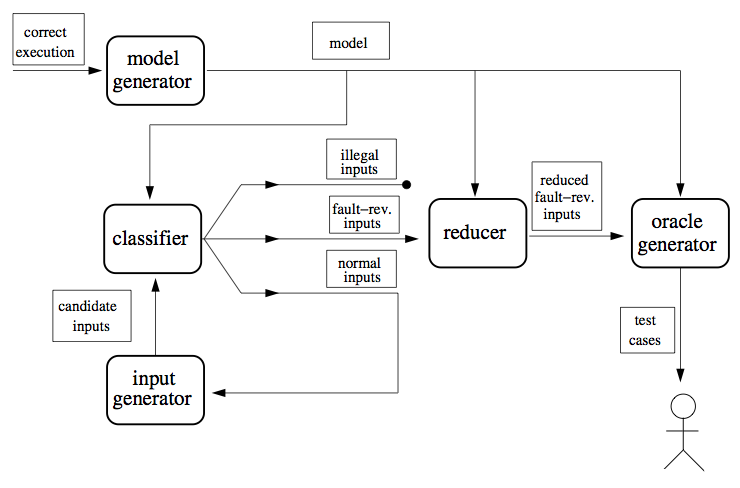
\includegraphics[width=15cm, height=10.5cm]{chapter3/eclat_working.png}
	\caption{Main component of Eclat contributing to generate test input~\cite{Pacheco2005}}
	\label{fig:eclat}
\end{figure}


The tool takes a software and a set of test cases for which the software runs properly. It creates an operational model, based on the correct software operations, and apply the test data. If the operational pattern of execution of the test data differs from the model, the following three outcomes may be possible: (a) a fault in the given SUT (b) model violation despite normal operation (c) illegal input which the program is unable to handle. In the second stage, reducer function is used to discard any redundant input, leaving only a single input per operational pattern. In the third stage, the acquired test inputs are converted into test cases and oracles are created to determine the success or failure of the test. \\

----- compared Eclat with JCrasher by executing nine programs on  both tools. ------ reported that Eclat performed better than JCrasher. On the average, Eclat selected 5.0 inputs per run out of which 30\% revealed faults while JCrasher selected 1.13 inputs per run out of which 0.92\% revealed faults. The limitation of Eclat is dependence on initial pool of correct test cases. Existence of errors in the pool leads to the creation of wrong operational model which adversely affects the testing process~\cite{Pacheco2007b}.   

%\subsection{JTest}
%Parasoft Jtest is a commercial tool that automatically generates and execute unit tests. It can be easily integrated to Java IDEs like Eclipse where it provide two main functionalities, i.e. Static Analysis, Unit testing and code coverage. [25]
%In static analysis Jtest takes a complete project or set of classes as input and compares it with a list of built-in rules. The statement violating any of these rules is an error. It also suggests probable fixes for the detected fault.
%For unit testing it takes a class as an input and processes a number of scenarios against it to generate and execute unit tests. Once unit tests are executed they become the part of regression test for future reference.
%Jtest also shows the code coverage of the program by colour coding the statements that are not executed by the unit tests.


\subsection{Randoop}
Random tester for Object Oriented Programs (RANDOOP) is the tool used for implementing FDRT technique~\cite{Pacheco2007b}. RANDOOP is a fully automatic tool, capable of testing Java classes and .Net binaries. It takes as input a set of classes, contracts, filters and time limit and gives output either as a suite of JUnit or NUnit for Java and .Net program respectively. Each unit test in a test suite is a sequence of method calls (hereafter referred as sequence). RANDOOP builds the sequence incrementally by randomly selecting a public method from the class under test and arguments for these methods are selected from the predefined pool in case of primitive types and a sequence or null value in case of reference type. RANDOOP maintains two sets called ErrorSeqs and NonErrorSeqs to record the feedback. It extends ErrorSeqs set in case of contract or filter violation and NonErrorSeqs set when no violation is recorded in the feedback. The use of this dynamic feedback evaluation at runtime brings an object to an interesting state. On test completion, ErrorSeqs and NonErrorSeqs are produced as JUnit/NUnit test suite. In terms of coverage and number of faults discovered, RANDOOP implementing FDRT was compared with JCrasher and JavaPathFinder and 14 libraries of both Java and .Net were evaluated~\cite{visser2004test}. The results showed that RANDOOP achieved more coverage than JCrasher in branch coverage and faults detection. It can achieve on par coverage with systematic approaches like JavaPathFinder. 

\subsection{QuickCheck}
QuickCheck~\cite{Claessen2000} is a lightweight random testing tool used for testing of Haskell programs~\cite{Hudak2007}. Haskell is a functional programming language where programs are evaluated by using expressions rather than statements as in imperative programming. In Haskell most of the functions are pure except the IO functions, thus main focus of the tool is on testing pure functions. QuickCheck is designed to have a simple domain-specific language of testable specifications embedded in Haskell. This language is used to define expected properties of the functions under test %- for example, reversing a list with single element must result in the same list.\\ %(author check the definition of pure functions)\\
\indent The QuickCheck takes function to be tested and properties of the program defined by tester (Haskell functions) as input. The tool uses built-in random generator to generate effective test data, however, to get adequate coverage in the case of custom data types, the testers can also develop their own generator. On executing the function with test data, the tester-defined-properties must hold for the function to be correct. Any violation of the defined properties suggest error in the function.



% The function is executed against the generated test data. The QuickCheck evaluates and declares a fault in the function where a test case violates the set properties.   



%\subsection{AgitarOne}
%AgitarOne is a commercial tool that automatically generates unit tests. It has a Junit Generator engine that can create 25,000 lines or more of Junit per hour [29]. It can be easily integrated into famous IDE like Eclipse. It takes as input, classes under test, time and optionally any knowledge or test cases that has a positive influence on the performance of the testing process. The generated Junit tests can be run from the same IDE and can also be used for later regression testing. The GUI interface is called a dashboard which provides in depth knowledge of the tests conducted, failures detected, alerts and the archieves of the tests conducted earlier. It also shows the coverage obtained after executing the Junits against the code under test.

\subsection{Autotest}
The Autotest, based on formal automated testing is used to test Eiffel language programs~\cite{Ciupa2007}. The Eiffel language uses the concept of contracts which is effectively utilized by Autotest. For example, the auto generated input is filtered using pre-conditions and unwanted test input is discarded. The contracts are also used as test oracle to determine if the test is pass or fail. Beside automated testing the Autotest also allows the tester to manually write the test cases to target specific section of the code. The Autotest may have a single method/class or suite of methods/classes as inputs, it then automatically generate test input data according to the requirement of the methods or classes.

\begin{figure}[h]
	\centering
	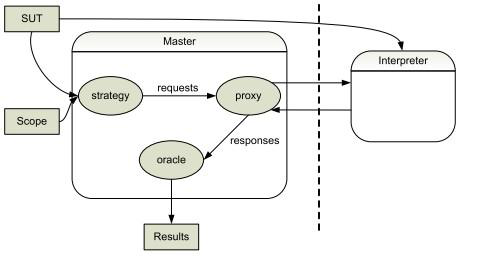
\includegraphics[width=13cm, height=7cm]{chapter3/autotest.png}
	\caption{Architecture of Autotest~\cite{Leitner2007}}
	\label{fig:autotest}
\end{figure}

\noindent According to Figure~\ref{fig:autotest}, the architecture of Autotest can be split into the following main parts:
\begin{enumerate}
\item \textbf{Testing Strategy:} It is a pluggable component where testers can fit any strategy according to the testing requirement. The strategy contains the directions for testing.%- for example what instructions should be executed on the SUT. Using the information the strategy synthesize test cases and forward it to the proxy. 
The default strategy creates test cases that uses random input to exercise the methods/classes under test.
\item \textbf{Proxy:} It handles inter-process communication. It receives execution requests from the strategy and forward these to the interpreter. The execution results are sent to the oracle.
\item \textbf{Interpreter:} It execute instructions on the SUT. The most common instructions include: create object, invoke routine and assign result. The interpreter is kept separate to increase robustness.
\item \textbf{Oracle:} It is based on contract-based testing. It evaluate the results to see if the contracts are satisfied. The outcome of the tests are formatted in HTML and stored on disk.
\end{enumerate}

\subsection{TestEra}
TestEra~\cite{Khurshid2004} is a novel framework for auto generation and evaluation of test inputs for a Java program. It takes methods specifications, integer value and the method under test as input. It uses pre-conditions of a method to generate all non isomorphic valid test inputs to the specified limit. The test inputs are executed on the method and the results are compared against the postconditions of the method serving as oracle. Any test case that fails to satisfy postcondition is considered as a fault. 

TestEra uses the Alloy modelling language~\cite{jackson2001micromodularity} to express constraints on test inputs and Alloy Analyser~\cite{jackson2000alcoa} to solve these constraints and generate test inputs. Alloy Analyzer performs the following three functions: (a) it translates Alloy predicates into propositional formulas, i.e. constraints where all variables are boolean (b) it evaluates the propositional formulas to find the outcome (c) it translates each outcome from propositional domain into the relational domain.

\begin{figure}[h]
	\centering
	\includegraphics[width=15cm, height=9cm]{chapter3/testera.png}
	\caption{Architecture of TestEra ~\cite{Khurshid2004}}
	\label{fig:testera}
\end{figure}


---TestEra and Korat are similar tools because they both uses program specifications to guide the auto generation of test inputs. However they are different from Jartege and AutoTest which uses specifications to filter and truncate the unnecessary random generated inputs. While the tools use program specifications differently for test input generation, they all uses it in a similar way for oracle. 


%Testera use specifications to guide the automatic generation of test inputs. It uses Alloy language for specification and Alloy Analyser to generate all non-isomorphic instances for a given size according to the specification automatically. Then, TestEra translate the instances to Java input as test cases for the program under test. After executing the test, TestEra then translate the outputs back to Alloy and Alloy Analyzer check the input and output against the correctness criteria given in Alloy. When it detects a violation, TestEra generates report in the form of concrete counterexamples. Figure 2.6 [50] illustrates the basic framework of TestEra.

\subsection{Korat} % please read thesis of khurshid in Mendeley in phd thesis section for more information.
Korat~\cite{Boyapati2002} is a novel framework for automated testing of Java programs based on the formal specifications~\cite{chang1999structural}. Korat and TestEra~\cite{Khurshid2004} were developed by the same team and perform specification based testing. The difference however is that Korat uses Java Modelling Language (JML) while TestEra uses Alloy Modelling Language for specifications. Moreover, Korat uses bounded-exhaustive testing in which the code is tested against all possible inputs within the given small bound~\cite{khurshid2001checking}.

Korat generate structurally complex inputs by solving imperative predicates. An imperative predicate is a piece of code that takes a structure as input and evaluates it to a boolean value. Korat takes imperative predicates and finitization value as inputs. It systematically explores the predicates input space and generates all non-isomorphic inputs for which the predicates return true. The core part of Korat monitors execution of the predicates on candidate inputs to filter out these fields accessed the particular fields during executions. These inputs are taken as test cases. Korat depends or developers written {\it repOK()} and {\it checkRep()} methods, where {\it repOK()} is used to check the class invariants and {\it checkRep()} is used to verify the post-conditions to validate the correctness of the test case. 

The key benefit of Korat and TestEra, representation level approaches, is that no existing set of operations are required to create input values and therefore they can achieve to create input values that may be difficult or impossible using a given set of operations. However, The only disadvantage to this approach is the requirement of significant amount of manual efforts \cite{pacheco2009directed}.    

%As the test start, it uses methods pre-condition to generate all non-isomorphic test cases up to a given size. It then executes each of the test case and compare the obtained results to the methods post-condition, which serves as an oracle to evaluate the correctness of each test case. 

%%%%%%%%%%%%%%%%%%%%%%%%%%%%%%%%%%%%%%%%%%%%%%
%													        %
%														 %			
% YETI Section Starts here									 %
%														 %		
%														 %
%%%%%%%%%%%%%%%%%%%%%%%%%%%%%%%%%%%%%%%%%%%%%%
\newpage

\section{YETI Overview}
York Extensible Testing Infrastructure (YETI), an automated random testing tool developed in Java, is capable of testing programs written in Java, JML and .NET languages~\cite{Oriol2010c}. YETI takes program byte code as input and execute it with random generated but syntactically-correct inputs to find a fault. It runs at a high level of performance with $10^6$ calls per minute on Java code. One of its prominent feature is Graphical User Interface (GUI), which make YETI user friendly and provides option to change testing process in real time. It can also distribute large testing tasks in cloud for parallel execution~\cite{Oriol2010}. The latest version of YETI can be downloaded from \url{https://code.google.com/p/yeti-test/downloads/list}. Figure \ref{fig:yetiOverview} briefly presents the working process of YETI. 
\\

\begin{figure}[h]
	\centering
	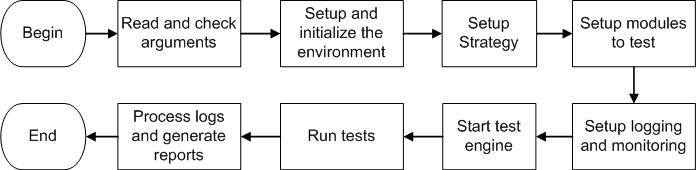
\includegraphics[width=15cm, height=4.5cm]{chapter3/yetiOverview.png}
	\caption{Working process of YETI}
	\label{fig:yetiOverview}
\end{figure}


\subsection{YETI Design}
YETI has been designed with the provision of extensibility for future growth. YETI enforces strong decoupling between test strategies and the actual language constructs, which adds new binding, without any modification in the available test strategies. YETI can be divided into three main parts on the basis of functionality: the core infrastructure, the strategy and the language-specific binding. Each part is briefly described below. 

\subsubsection{Core Infrastructure}
The core infrastructure is responsible for test data generation, test process management and test report generation. The core infrastructure is split into four packages: yeti, yeti.environments, yeti.monitoring, yeti.strategies. The package yeti uses classes from yeti.monitoring and yeti.strategies packages and calls classes in the yeti.environment package as shown in the Figure \ref{fig:yetiCore}. 

\begin{figure}[h]
	\centering
	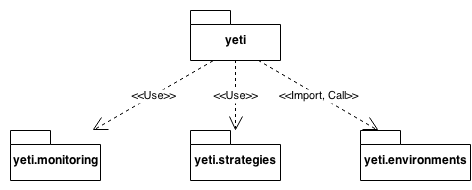
\includegraphics[width=15cm, height=7cm]{chapter3/yetiCore.png}
	\caption{Main packages of YETI with dependencies }
	\label{fig:yetiCore}
\end{figure}

The most essential classes included in the YETI core infrastructure are:
\begin{enumerate}
\item {\textbf{Yeti class:}} It is the entry point to YETI and contains the main method. It parses the arguments, sets up the environment, initializes the testing and delivers the reports of the test results.
\item {\textbf{YetiLog class:}} It prints debugging and testing logs. 
\item {\textbf{YetiLogProcessor class:}} It is an interface for processing testing logs.
\item {\textbf{YetiEngine class:}} It binds YetiStrategy and YetiTestManager together, which carry out the actual testing process.
\item {\textbf{YetiTestManager class:}} It makes the actual calls based on the YetiEngine configuration, activate the YetiStrategy to generate test data and select the routines.
\item {\textbf{YetiProgrammingLanguageProperties class:}} It is a place holder for all language related instances.
\item {\textbf{YetiInitializer class:}} It is an abstract class for test initialization.
\end{enumerate}

\subsubsection{Strategy}
The strategy defines a specific way to generate test inputs. This part contains six essential strategies stated below.
\begin{enumerate}
\item {\textbf{YetiStrategy class:}} It is an abstract class which provides interface for every strategy in YETI.
\item {\textbf{YetiRandomStrategy class:}} It implements the random strategy and generates random values for testing. The strategy gives choice to the user to adjust null values probability and the percentage of creating new objects for the test session. 
\item {\textbf{YetiRandomPlusStrategy class:}} It extends the random strategy by adding interesting values to the list of test values. The strategy gives the choice to the user to select the percentage of interesting values used in the test session.
\item {\textbf{DSSRStrategy class:}} It extends random+ strategy by adding the values surrounding the fault value. The strategy is described in detail in Chapter~\ref{chap:DSSR}.
\item {\textbf{ADFDStrategy class:}} It extends random+ strategy by adding the feature of graphical representation of faults and their domains. The strategy is described in detail in Chapter~\ref{chap:ADFD}.
\item {\textbf{YetiRandomDecreasingStrategy class:}} It extends the random+ strategy by setting the probability value to starts at 100\% and ends at 0\% when the test finishes.
\item {\textbf{YetiRandomPeriodicStrategy class:}} It extends random+ strategy by setting the probability in such a way that it decreases and increases randomly during test session.
\end{enumerate}

\subsubsection{Language-specific Binding}
The language-specific binding provides support for modelling a programming language. They are language independent and need to be extended for supporting a new language.
\begin{enumerate}
\item {\textbf{YetiVariable class:}} It is a sub class of YetiCard representing a variable in YETI.
\item {\textbf{YetiType class:}} It denotes type of data including Integer, String, Boolean etc.
\item {\textbf{YetiRoutine class:}} It is a super type of routines which represents functions, methods and constructors. A routine is given a name, a return type and a list of its arguments types.
\item {\textbf{YetiModule class:}} It represents a module under test. It stores a list of the module’s routines to test. 
\item {\textbf{YetiName class:}} It represents a unique name which is assigned to each instance of YetiRoutine.
\item {\textbf{YetiCard class:}} It is a YETI specific term which map to a wildcard or to a YetiVariable. It has a specific type and an identifier name.
\item {\textbf{YetiIdentifier class:}} It represents an identifier for an instance of a YetiCard.
\end{enumerate}
% if java binding example is required or instead of adding new steps if you want to show only java binding then for material check the msc thesis page 40 of test c code with Yeti.

\subsection{Construction of Test Cases}
YETI construct test cases by creating objects of the classes under test and randomly calling its methods with random inputs according to its parameter's-space. YETI split input values into two types i.e. primitive data types and user defined classes. For Java primitive data types, which includes short, byte, char, int, float, double, long etc., YETI, in its simplest random strategy, calls {\it Math.random()} method to generate an arithmetic value which is converted to the required type using casting rule of Java language. However, if the method under test needs an object of a user-defined class as a parameter then YETI calls its constructor or method to generate object of that class at run time. It may be possible that the constructor require another object and in that case YETI will recursively calls the constructor of that object. This process is continued until an object with blank constructor, constructor with only primitive types or the set level of recursion is reached.

\subsection{Command-line Options}
While YETI GUI launcher has been developed during this research study, to take maximum benefit of the available options one still need to launch YETI from CLI mode. These command-line options are case insensitive and can be provided as input to the tool in CLI mode in any order. For example, to save processing power and reduce overhead for a test session, command line option -nologs can be use to bypass real-time logging. The following table \ref{table:cliOptions} describes few of the most common command-line options available in YETI. 

\begin{table}[h]
%\scriptsize
\caption{YETI command line options} % title of Table
\smallskip
\centering % used for centering table
\begin{tabular}{|l|l|} % centered columns (4 columns)
\hline

Options									&Purpose 			\\ \hline
-java										&Test programs coded in Java	 	\\ \hline
-jml										&Test programs coded in JML			\\ \hline
-dotnet									&Test programs coded in .NET		\\ \hline
-ea											&To check code assertions \\ \hline
-nTests									&\vtop{\hbox{\strut Specify number of tests after} \hbox{\strut which the test stops}}	\\ \hline
-time										&\vtop{\hbox{\strut Specify time in seconds or minutes} \hbox{\strut after which the test stops}}\\ \hline
-testModules						&Specify one or more modules to test 	\\ \hline
-rawlogs								&Prints real time logs during test \\ \hline
-nologs									&Omit real time logs and print end result only\\ \hline
-yetiPath								&Specify path to the test modules\\ \hline
-gui										&Show test session in GUI\\ \hline
-DSSR										&\vtop{\hbox{\strut Specify Dirt Spot Sweeping Random} \hbox{\strut strategy for this session}}\\ \hline
-ADFD										&\vtop{\hbox{\strut Specify Automated Discovery of Failure} \hbox{\strut Domain strategy for this session}}\\ \hline
-random									&Specify random test strategy for this session\\ \hline
-randomPlus							&Specify random plus test strategy for this session\\ \hline
-randomPlusPeriodic			&\vtop{\hbox{\strut Specify random plus periodic test} \hbox{\strut strategy for this session}}\\ \hline
-nullProbability				&\vtop{\hbox{\strut Specify probability of inserting} \hbox{\strut null as input value}}\\ \hline
-newInstanceProability	&\vtop{\hbox{\strut Specify probability of inserting} \hbox{\strut new object as input value}}\\ \hline

\hline %inserts single line
\end{tabular}
\bigskip
\label{table:cliOptions} % is used to refer this table in the text
\end{table}


\subsection{YETI Execution}
YETI being developed in Java is highly portable and can easily run on any operating system with Java Virtual Machine (JVM) installed. YETI can be executed from both command line and GUI. To build and execute YETI, it is necessary to specify the {\it project} and all the associated {\it .jar library files} particularly {\it javassist.jar} in the {\it CLASSPATH} to help JVM in identifying the YETI source. The typical command to invoke YETI is given in Figure~\ref{fig:yeticommand}.

\begin{figure}[h!]
	\centering
	\frame{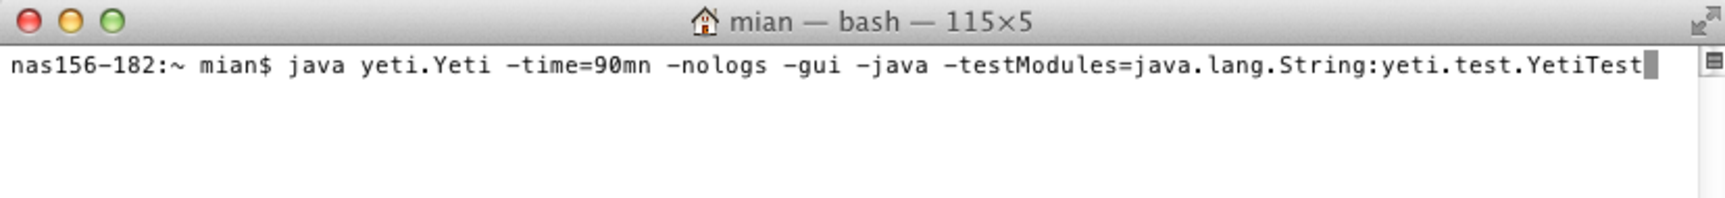
\includegraphics[width= 14cm, height = 1.8cm]{chapter3/yetiCommandCLI.pdf}}
	\caption{Command to launch YETI from CLI}
	\label{fig:yeticommand}
\end{figure}

 In this particular command YETI tests java.lang.String and yeti.test.YetiTest modules for 90 minutes using the default random strategy. For details of other options please see table \ref{table:cliOptions}. Alternately, runnable jar file by the name {\it YetiLauncher} is also available to launch YETI from GUI. However, till the writing of this thesis, the GUI version of YETI only supports the basic options of YETI execution. Figure \ref{fig:yetiLauncher} shows the equivalent of above command in GUI mode.

\begin{figure}[h]
	\centering
	\frame{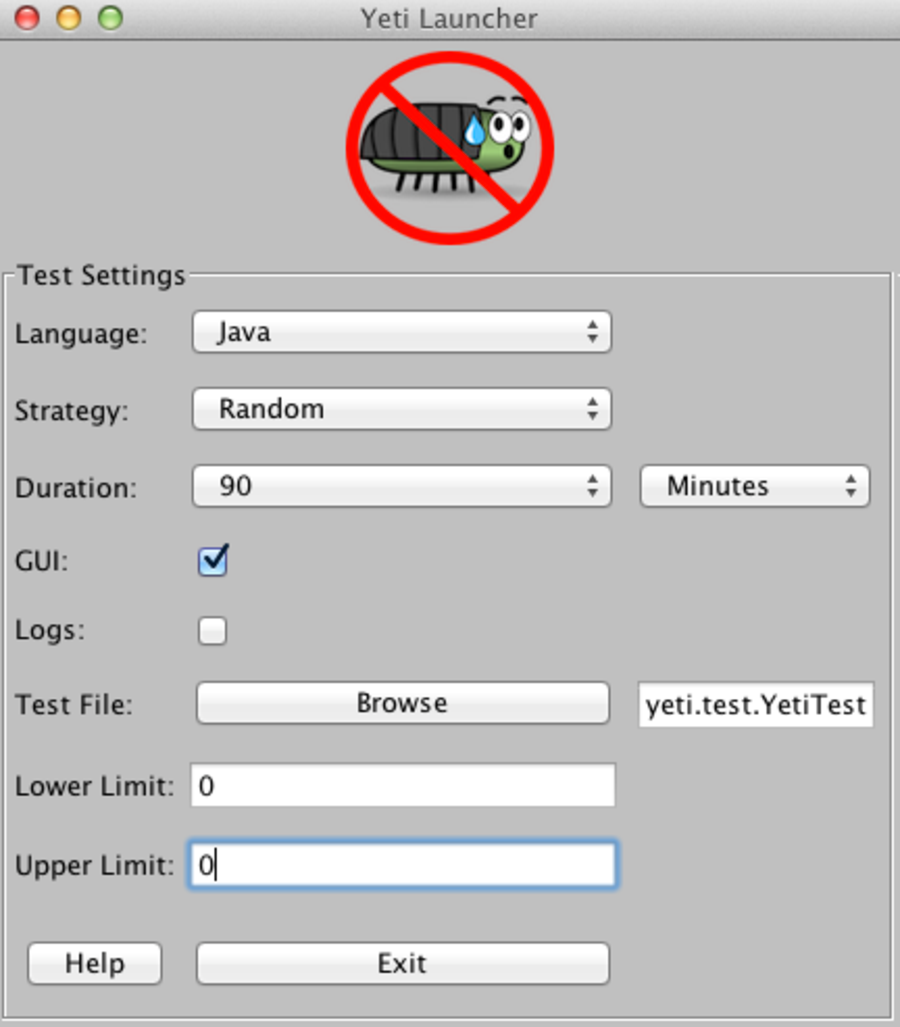
\includegraphics[width= 7cm, height = 8cm]{chapter3/yetiCommandGUI.pdf}}
	\caption{GUI launcher of YETI}
	\label{fig:yetiLauncher}
\end{figure}


As a result of both the above commands YETI launch its own GUI window and start testing the assigned programs. 

\subsection{YETI Test Oracle}
Oracles in YETI are language dependant. YETI uses two approaches for oracle (pass/fail judgement). In the presence of program specifications, YETI checks for inconsistencies between the code and the specifications. In the absence of specifications YETI checks for assertion violations if assert statements are included by the programmer. However in the absence of both specifications and assertions YETI performs robustness testing that considers any undeclared runtime exceptions as failures. 

%If code contracts are available, YETI uses them as oracle, however, in their absence YETI uses undeclared runtime exceptions of the underlying language as oracle. The test cases revealing errors are reproduced at the end of each test session for unit and regression testing.
%YETI deals with the oracle problem in two ways. If available, it uses code-contracts as oracles, however in the absence of contracts it uses runtime exceptions as errors which is also known as robustness testing.

\subsection{YETI Report}
YETI gives a complete test report after execution of each test. The report contain all the successful calls with the name of the routines and the unique identifiers for the parameters in each execution. These identifiers are recorded with the assign value to help in debugging the identified fault. 
\begin{figure}[h]
	\centering
	\frame{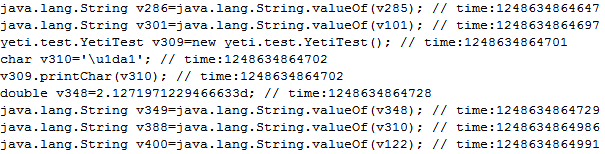
\includegraphics[width= 14cm, height = 4cm]{chapter3/yetiReport1.png}}
	\caption{YETI successful method calls}
\end{figure}

YETI separates the bugs from successful executions to simplify the test report. This approach helps debuggers to easily track the origin of the problem and rectify it. When a bug is identified during testing YETI saves that state and present it in the bug report. The information includes all the identifiers of the parameters the method call had at the time of execution. It also report the time at which the exception occurs.

\begin{figure}[h]
	\centering
	\frame{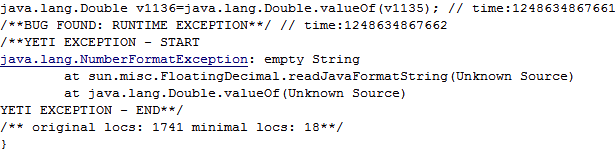
\includegraphics[width= 14cm, height = 4cm]{chapter3/yetiReport2.png}}
	\caption{YETI bug reports.}
\end{figure}

\subsection{YETI Graphical User Interface}
YETI supports a GUI that not only allows test engineers to monitor the current test session but also to modify its characteristics in real time during test execution. It is useful to have the facility of modifying or aborting the test parameters at run time and observing the test behaviour in response. The Figure \ref{fig:yetiGUI} present the YETI GUI comprising of six numbered windows (the windows are labelled for illustration purposes only).

\begin{figure}[h]
	\centering
	\frame{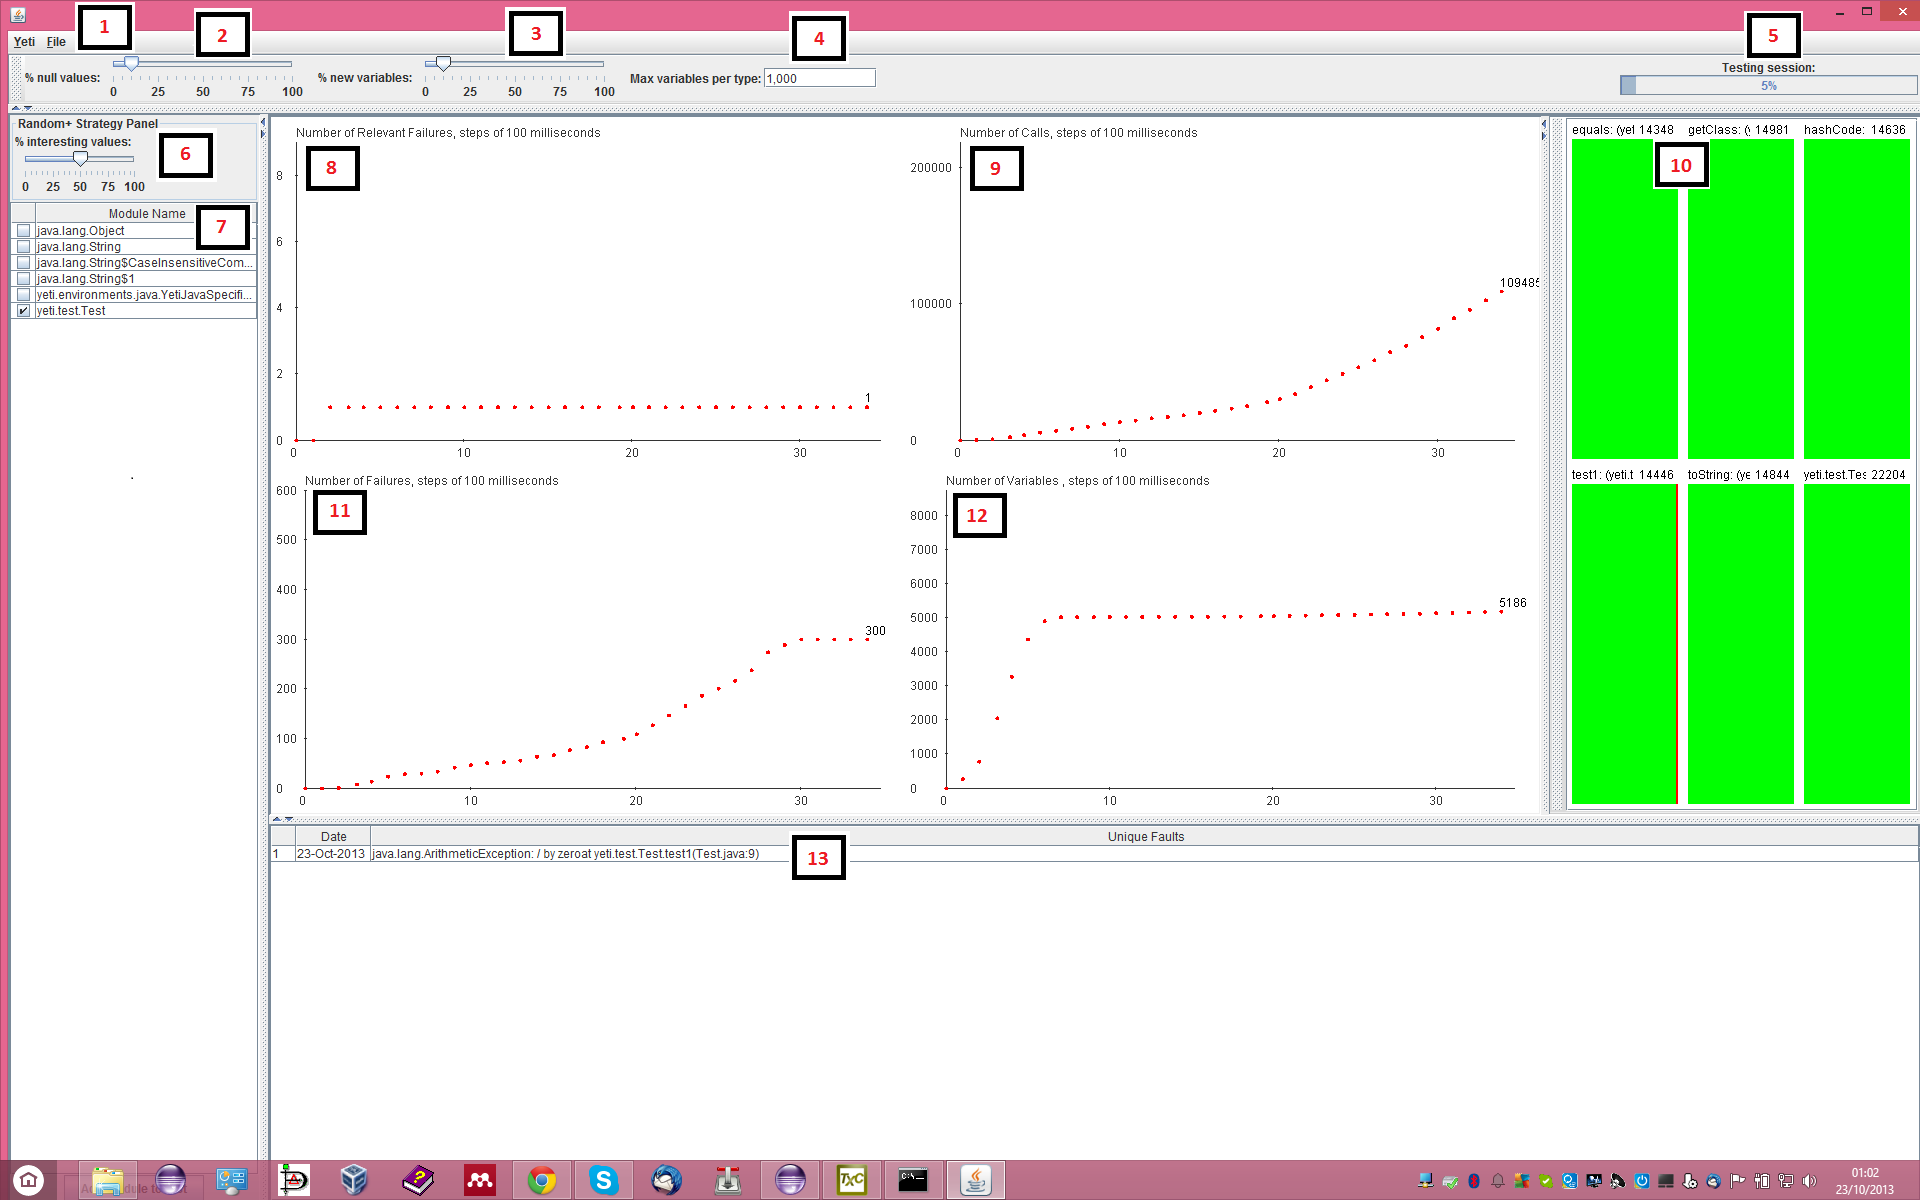
\includegraphics[width= 15cm, height = 10cm]{chapter3/yetiGUI.png}}
	\label{fig:yetiGUI}
	\caption{GUI of YETI}
\end{figure}

\begin{enumerate}

\item Menu bar:
\begin{enumerate}
\item Yeti menu:
\item File menu:
\end{enumerate}
\item Standard toolbar:
\begin{enumerate}
\item Slider: “\%null values” displays probability to use a null instance at each variable. The probability is set before the testing by using the option –probabilityToUseNullValue. The default probability is 1. 
\item Slider “\% new variables” displays probability to create new instances at each call. Same as “\%null values”, it is set before the testing by using the option –newInstanceInjectionProbability and the default value is 1. 
\item Text box “Max variables per type” displays the cap on the number of instances for any given type. User can modify the sliders and text box during the testing according different test strategies. 
\item The progress bar “Testing session” indicates the percentage of the test progress.
\end{enumerate}
\item Module Name shows the list of the modules under the test. The
modules with ticks are the modules under test. The module names also show all the
class names in the test module.
\item displays the number of unique of bugs detect in the module under
test over time.
\item displays the number of calls to the module under test over time.
\item displays the number of failures over time. They are not both related
to the module under test.
\item displays the number of object instances created by YETI over time.
\item displays all the routines in the module under test with a rectangle.
Each rectangle presents the results of calls of the routine. The rectangle can have in 4 colors. Black indicates no any calls of this routine. Green indicates that has successful calls of this routine. Red indicates that this routine is called unsuccessfully which means that the call to this routine results in an exception. Yellow indicates undecidable calls, for example if a call cannot finish in predefined time and Yeti stops this call, in this case yeti cannot decide this call is successful or unsuccessful. The text next the routines name show how many calls of this routine and text displays percentage of passed, failed and undescided when the cursor over the rectangle.
\item displays a table which contains the unique faults are detected by Yeti. It records the detail of exceptions.
\item Window No 1 displays the failures of the tested module over time.
\item Window No 2 displays the total number of failures over time. These may be generated from calls not related to the tested module.
\item Window No 3 displays the total number of calls to the tested module over time. 
\item Window No 4 displays the total number of variables generated by YETI over time.
\item Window No 5 displays colored rectangles: one for each constructor and method under test. Each rectangle represents the calls to a constructor or a method.
\item The colors in a rectangle have the following meaning:
\item Green indicates successful calls (✓). A successful call is one that does not raise an exception or if it does, the method or the constructor declares to throw it.
\item Red indicates failed calls (X). A failed call results from raised RuntimeException or one of its subclasses.
\item Yellow indicates “undecidable” calls (?). A call is “undecidable” if for some reason it takes too long to complete and needs to be stopped, or if a YetiSecurityException (custom exception in YETI) is thrown.
\end{enumerate}


\subsection{Summary}
In this chapter we define random testing and the various ways of performing random testing. We then showed how the automated testing tools implement random technique for software testing. Finally the chapter explains in detail the YETI which is being used in this study. The main features of all the tools are noted in the following table.

\begin{sidewaystable}
    \centering
    \caption{Summary of automated testing tools}
   \begin{tabular}{|l|l|l|l|l|l|}
\hline

Tool 				& Language																								& Input  																																			& Strategy 																																											 				& Output		  																								& Benefits																															\\ \hline
JCrasher	  & Java, JML																								& Program																																			& \vtop{\hbox{\strut Method type to predict input,}\hbox{\strut Randomly find values of crash}}  				& TC																													& \vtop{\hbox{\strut Automated TC, Use} \hbox{of Heuristic Rules}} 	 \\ \hline
Jartege			& Java																										& Classes																																			& \vtop{\hbox{\strut Random strategy with controls}\hbox{\strut like weight etc.}} 							 				& TC, RT 																											& Quick, automated																									 \\ \hline
Eclat				& Java																										& Classes, pass TC 																														& \vtop{\hbox{\strut Create model from TC, execute}\hbox{\strut each candidate on the model}} 					& Faulty TC 																									& \vtop{\hbox{\strut produce output text,} \hbox{JML}}									\\ \hline
Quickcheck	& Haskell																									&	\vtop{\hbox{\strut Specifications}  \hbox{\strut and Functions}}	  			  & \vtop{\hbox{\strut Specification} \hbox{\strut hold to random TC?}} 											 						& Pass/Fail																										& \vtop{\hbox{\strut Easy to use, program} \hbox{documentation}}				\\ \hline
Randoop 		& Java, .NET																							& \vtop{\hbox{\strut Specifications,} \hbox{\strut code and time}}					  & \vtop{\hbox{\strut Generate and execute methods} \hbox{\strut \& give feedback for next generation}} 	& Fault TC, RT 																								& 																																\\ \hline
AgitarOne		& Java																										& \vtop{\hbox{\strut Package, time}   \hbox{\strut and manual TC}}						& \vtop{\hbox{\strut Analyse SUT with auto and} \hbox{\strut provided data in specified time}} 					& TC, RT																											& \vtop{\hbox{\strut Eclipse plug-in} \hbox{\& easy to use}}  			 \\ \hline
AutoTest		& Java																										& \vtop{\hbox{\strut Classes, time}   \hbox{\strut and manual TC}} 						& \vtop{\hbox{\strut Heuristic rules} \hbox{\strut to evaluate contracts}} 															& violations, RT 																							& \vtop{\hbox{\strut GUI in HTML,} \hbox{easy to use}} 								\\ \hline
TestEra			& Java																										& \vtop{\hbox{\strut Specifications,} \hbox{\strut integer \& manual TC}}			& \vtop{\hbox{\strut Check contracts} \hbox{\strut with specifications}} 																& Contracts violations 																				& \vtop{\hbox{\strut short report with} \hbox{faulty TC only}} 					\\ \hline
Korat 			& Java																										& \vtop{\hbox{\strut Specifications}  \hbox{\strut and manual tests}}					& \vtop{\hbox{\strut Check contracts} \hbox{\strut with specifications}}																& Contracts violations 																				& \vtop{\hbox{\strut GUI, short report} \hbox{with faulty TC only}} 	 \\ \hline
YETI 				& \vtop{\hbox{\strut Java, .NET,}  \hbox{\strut JML}} 		& Code, Time 																																  & RandomPlus, Random 																																										& \vtop{\hbox{\strut Traces of found } \hbox{\strut faults}}	& \vtop{\hbox{\strut GUI, give faulty} \hbox{examples, Quick}} 			 \\ \hline %inserts single line
\end{tabular}
\label{table:Tools}
\end{sidewaystable}


%\begin{figure}[h]
%	\centering
%	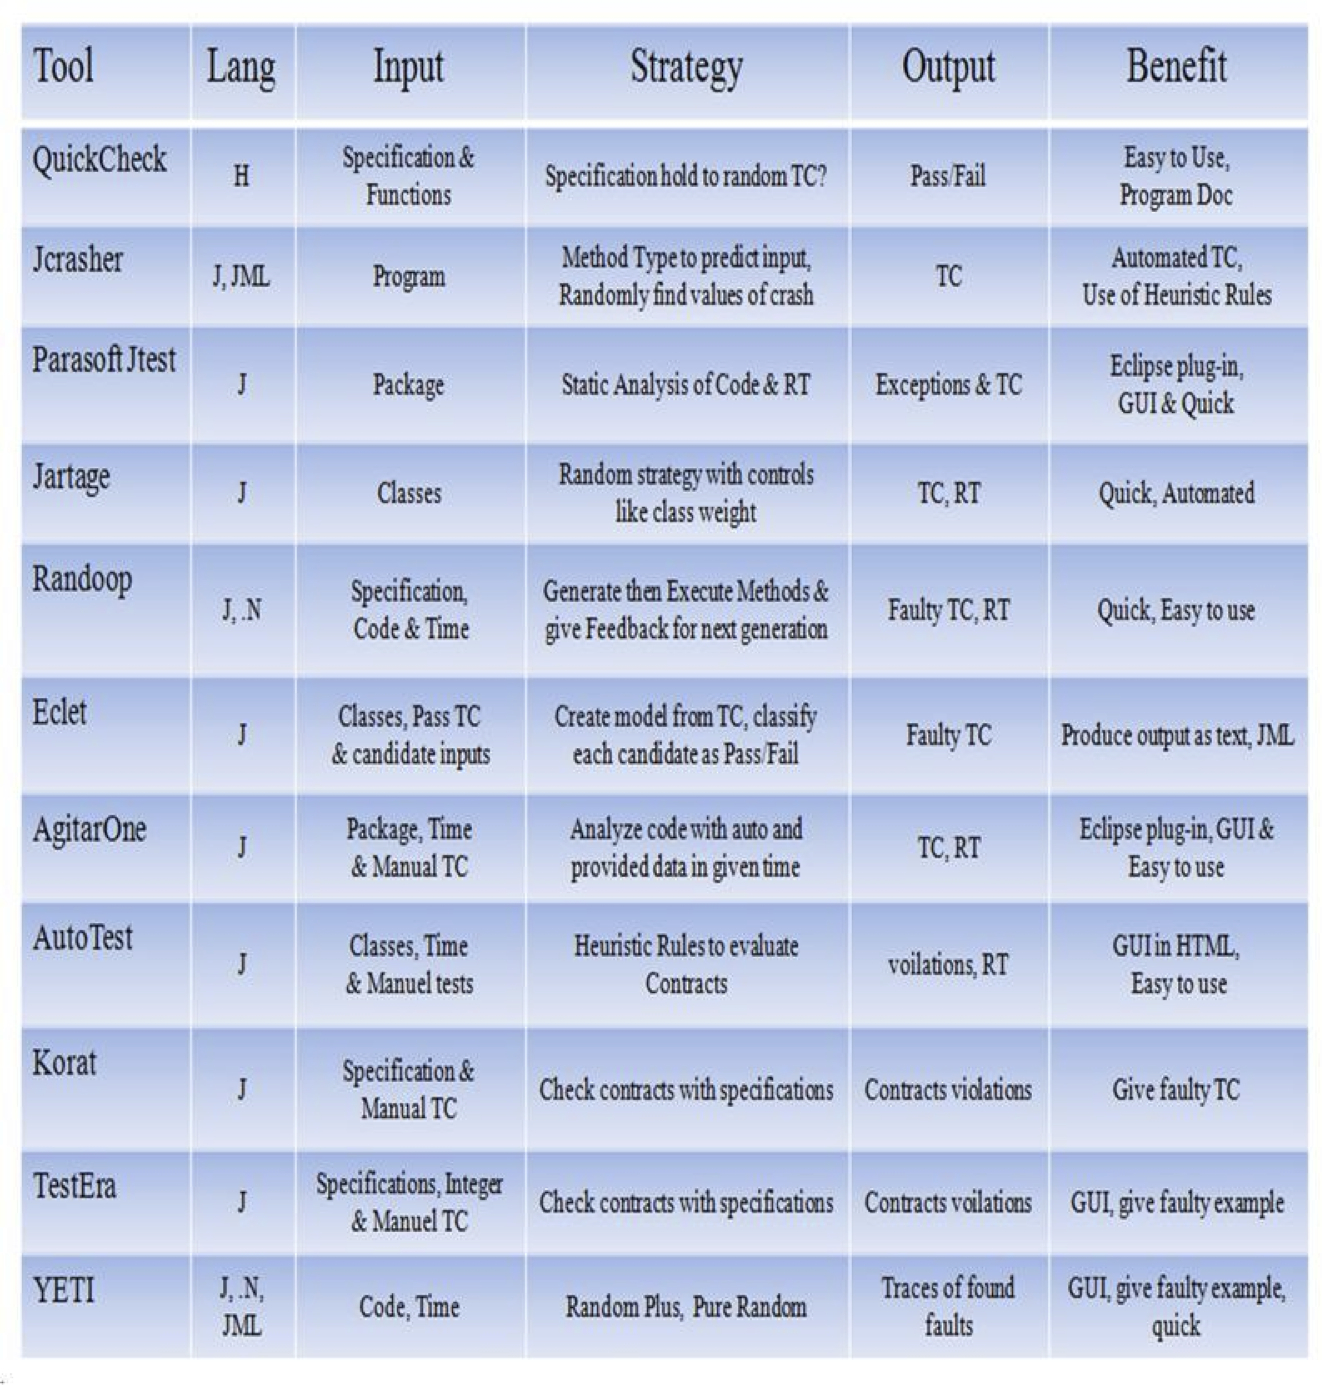
\includegraphics[scale=0.6]{chapter2/tools.jpg}
%	\caption{Summary of automated testing tools}
%\end{figure}




%\section{Conclusion}


% ------------------------------------------------------------------------


%%% Local Variables:
%%% mode: latex
%%% TeX-master: "../thesis"
%%% End:

\chapter{Dirt Spot Sweeping Random Strategy}
\label{chap:DSSR}
%\ifpdf
%    \graphicspath{{Dssr/DssrFigs/PNG/}{Dssr/DssrFigs/PDF/}{Dssr/DssrFigs/}}
%\else
 %   \graphicspath{{Dssr/DssrFigs/EPS/}{Dssr/DssrFigs/}}
%\fi

%%%%%%%%%%%%%%%%%    INTRODUCTION   %%%%%%%%%%%%%%%%%%%%
\section{Introduction}\label{sec:intro4}
The success of a software testing technique is mainly based on the number of faults it discovers in the SUT. An efficient testing process discovers the maximum number of faults in a minimum possible time. Exhaustive testing, where software is tested against all possible inputs, is mostly not feasible because of the large size of the input domain, limited resources and strict time constraints. Therefore, strategies in automated software testing tools are developed with the aim to select more fault-finding test input from input domain for a given SUT. Producing such targeted test input is difficult because each system has its own requirements and functionality.

Chan et al.~\cite{Chan1996} discovered that there are patterns of failure-causing inputs across the input domain. They divided the patterns into point, block and strip patterns on the basis of their occurrence across the input domain. Chen et al.~\cite{Chen2008} found that the performance of random testing can be increased by slightly altering the technique of test case selection. In adaptive random testing, they found that the performance of random testing increases by up to 50\% when test input is selected evenly across the whole input domain. This was mainly attributed to the better distribution of input which increased the chance of selecting inputs from failure patterns. Similarly Restricted Random Testing \cite{Chan2002}, Feedback directed Random Test Generation \cite{Pacheco2007}, Mirror Adaptive Random Testing \cite{Chen2003} and Quasi Random Testing \cite{Chen2005} stress the need for test case selection covering the whole input domain to get better results.

In this chapter we take the assumption that for a significant number of classes failure domains are contiguous or are very close by. From this assumption, we devised the Dirt Spot Sweeping\footnote{The name refers to the cleaning robots strategy which insists on places where dirt has been found in large amount.} Random (DSSR) strategy  which starts as a random+ strategy --- a random strategy focusing more on boundary values. When a new failure is found, it increases the chances of finding more faults using neighbouring values. As in previous studies~\cite{oriol2012law} we approximate faults with unique failures. Since this strategy is an extension of random testing strategy, it has the full potential to find all unique failures in the program, but additionally we expect it to be faster at finding unique failures, for classes in which failure domains are contiguous, as compared with random (R) and random+ (R+) strategies.

We implemented the DSSR strategy in the random testing tool YETI\footnote{\url{http://www.yetitest.org}}. To evaluate our approach, we tested 30 times each one of the 60 classes of 32 different projects from the Qualitas Corpus\footnote{\url{http://www.qualitascorpus.com}} with each of the three strategies R, R+ and DSSR. We observed that for 53\% of the classes all three strategies find the same unique failures, for remaining 47\% DSSR strategy perform up to 33\% better than random strategy and up to 17\% better than random+ strategy.
We also validated the approach by comparing the significance of these results using t-tests and found out that for 7 classes DSSR was significantly better than both R+ and R, for 8 classes DSSR performed similarly to R+ and significantly better than R, while in 2 cases DSSR performed similarly to R and significantly better than R+. In all other cases, DSSR, R+ and R do not seem to perform significantly differently.
Numerically, the DSSR strategy found 43 more unique failures than R and 12 more unique failures than R+ strategy. 

%The rest of this paper is organised as follows: \\ Section~\ref{sec:dssr} describes the DSSR strategy. Section~\ref{sec:imp} presents implementation of the DSSR strategy. Section~\ref{sec:eval} explains the experimental setup. Section~\ref{sec:res} shows results of the experiments. Section~\ref{sec:discussion3} discusses the results. Section~\ref{sec:rw} presents related work and Section~\ref{sec:conc}, concludes the study.




%%%%%%%%%%%%%%%%%    DIRT SPOT SWEEPING STRATEGY  %%%%%%%%%%%%%%%

\section{Dirt Spot Sweeping Random Strategy}\label{sec:dssr}
The new software testing technique named, Dirt Spot Sweeping Random (DSSR) strategy combines the random+ strategy with a dirt spot sweeping functionality. It is based on two intuitions. First, boundaries have interesting values and using these values in isolation can provide high impact on test results. Second, faults and unique failures reside in contiguous block and strip pattern. If this is true, DSS increase the performance of the test strategy. Before presenting the details of the DSSR strategy, it is pertinent to review briefly the Random and the Random+ strategy.

\subsection{Random Strategy (R)}
The random strategy is a black-box testing technique in which the SUT is executed using randomly selected test data. Test results obtained are compared to the defined oracle, using SUT specifications in the form of contracts or assertions. In the absence of contracts and assertions the exceptions defined by the programming language are used as test oracles. Because of its black-box testing nature, this strategy is particularly effective in testing softwares where the developers want to keep the source code secret~\cite{Chen2010}. The generation of random test data is comparatively cheap and does not require too much intellectual and computational efforts~\cite{Ciupa2009, Ciupa2008}. It is mainly for this reason that various researchers have recommended random strategy for automated testing tools \cite{Ciupa2008a}. YETI \cite{Oriol2010b, Oriol2010}, AutoTest \cite{Ciupa2007, Leitner2007}, QuickCheck \cite{Claessen2000}, Randoop \cite{Pacheco2007}, JArtege \cite{Oriat2004} are some of the most common automated testing tools based on random strategy.

\indent Efficiency of random testing was made suspicious with the intuitive statement of Myers \cite{Myers1979} who termed random testing as one of the poorest methods for software testing. However, experiments performed by various researchers, \cite{Ciupa2007, Duran1981, Duran1984, hamlet1994, Ntafos2001} have proved experimentally that random testing is simple to implement, cost effective, efficient and free from human bias as compared to its rival techniques.

Programs tested at random typically fail a large number of times (there are a large number of calls), therefore, it is necessary to cluster failures that likely represent the same fault. The traditional way of doing it is to compare the full stack traces and error types and use this as an equivalence class~\cite{Ciupa2007,Oriol2012} called a unique failure. This way of grouping failures is also used for random+ and DSSR.

\subsection{Random Plus Strategy (R+)}
The random+ strategy~\cite{Leitner2007} is an extension of the random strategy. It uses some special pre-defined values which can be simple boundary values or values that have high tendency of finding faults in the SUT. Boundary values~\cite{Beizer1990} are the values on the start and end of a particular type. For instance, such values for \verb+int+ could be \verb+MAX_INT+, \verb+MAX_INT-1+, \verb+MAX_INT-2+; \verb+MIN_INT+, \verb-MIN_INT+1-, \verb-MIN_INT+2-. These special values can add a significant improvement to any testing method. For example:

\begin{lstlisting}
public void test (int arg) {
arg = arg + 1;
int [] intArray = new intArray[arg];
...
}
\end{lstlisting}

In the above piece of code, on passing interesting value \verb+MAX_INT+ as argument the code increment it by 1 making it a negative value and thus an error is generated when the system try to build an array of negative size. 

Similarly, the tester might also add some other special values that he considers effective in finding faults for the SUT. For example, if a program under test has a loop from -50 to 50 then the tester can add -55 to -45, -5 to 5 and 45 to 55 to the pre-defined list of special values. This static list of interesting values is manually updated before the start of the test and has slightly high priority than selection of random values because of more relevance and high chances of finding faults for the given SUT. These special values have high impact on the results, particularly for detecting problems in specifications~\cite{Ciupa2008}.


\subsection{Dirt Spot Sweeping (DSS)}
Chan et al.~\cite{Chan1996} found that there are patterns of failure-causing inputs across the input domain. Figure \ref{fig:patterns3} shows these patterns for two dimensional input domain. They divided these patterns into three types called points, block and strip patterns. The black area (points, block and strip) inside the box show the input which causes the system to fail while white area inside the box represent the genuine input. Boundary of the box (black solid line) surrounds the complete input domain and represents the boundary values. They argue that a strategy has more chances of hitting these fault patterns if test cases far away from each other are selected. Other researchers~\cite{Chan2002, Chen2003, Chen2005}, also tried to generate test cases further away from one another targeting these patterns and achieved better performance. Such increase in performance indicate that faults more often occur contiguous across the input domain. In Dirt Spot Sweeping we propose that if a value reveals fault from the block or strip pattern then for the selection of the next test value, DSS may not look farthest away from the known value and rather pick the closest test value for the next couple of tests to find another fault from the same region.

\begin{figure}[ht]                                    
\centering
\includegraphics[width= 8cm,height=2.5cm]{chapter4/ART_Patterns.png}
\caption{Failure patterns across input domain~\cite{Chen2008}}
\label{fig:patterns3}
\end{figure}

Dirt spot sweeping is the part of DSSR strategy that comes into action when a failure is found in the system. On finding a failure, it immediately adds the value causing the failure and its neighbouring values to the existing list of interesting values. For example, in a program when the \verb+int+ type value of 50 causes a failure in the system then spot sweeping will add values from 47 to 53 to the list of interesting values. If the failure lies in the block or strip pattern, then adding it's neighbouring values will explore other failures present in the block or strip. As against random plus where the list of interesting values remain static, in DSSR strategy the list of interesting values is dynamic and changes during the test execution of each program.

\begin{figure}[ht]
\centering
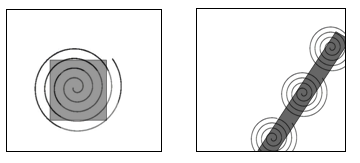
\includegraphics[width=8cm,height=2.2cm]{chapter4/block2.png}
\caption{DSSR covering block and strip pattern}
\label{fig:block2}
\end{figure}

Figure \ref{fig:block2} shows how DSS explores the failures residing in the block and strip patterns of a program. The coverage of block and strip pattern is shown in spiral form because first failure leads to second, second to third and so on till the end. In case the failure is positioned on the point pattern then the added values may not be effective because point pattern is only an arbitrary failure point in the whole input domain.

\subsection{Structure of the Dirt Spot Sweeping Random Strategy}

The DSSR strategy continuously tracks the number of failures during the execution of the test. This tracking is done in a very effective way with zero or minimum overhead to keep the overhead up to bare minimum~\cite{Leitner2009}. The test execution is started by R+ strategy and continues till a failure is found in the SUT after which the program copies the values leading to the failure as well as the surrounding values to the variable list of interesting values. 

\begin{figure}[ht]
\centering
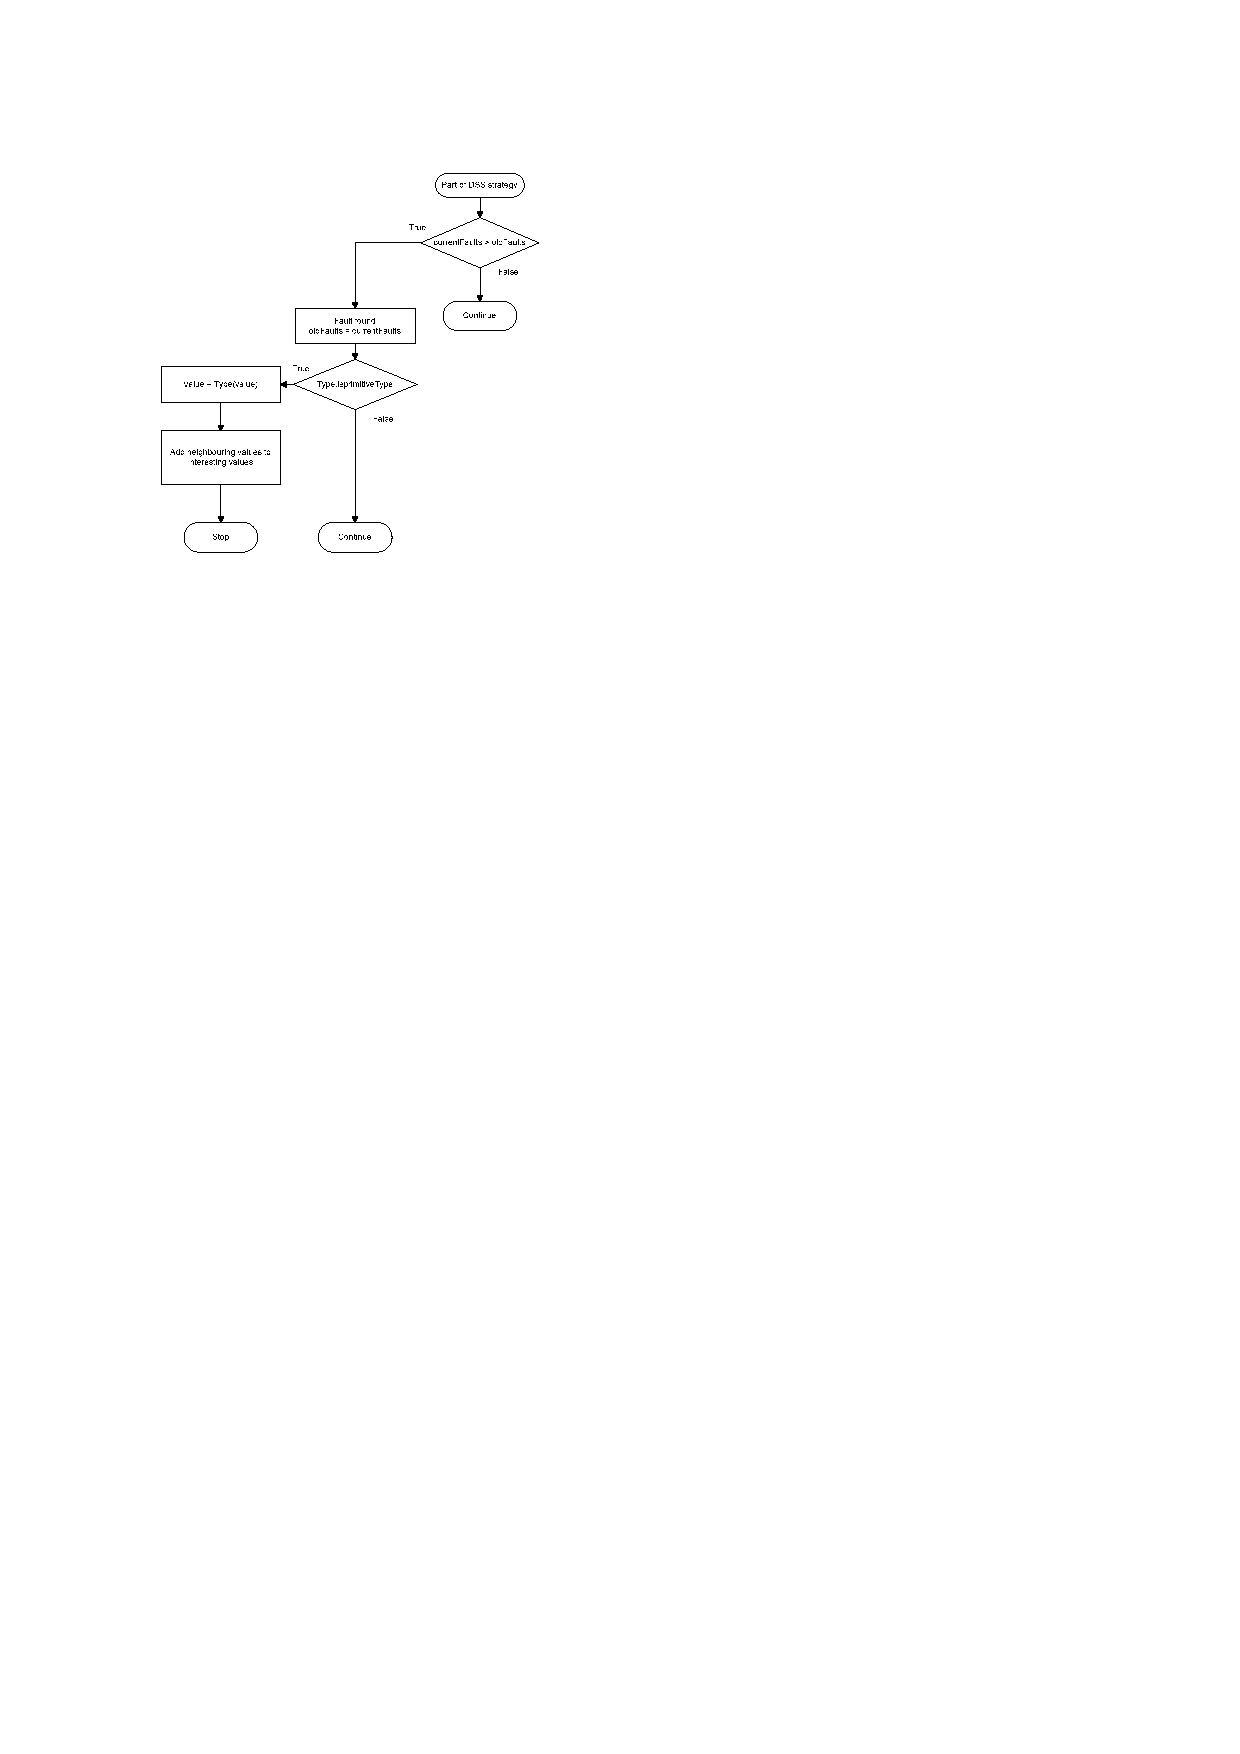
\includegraphics[width=10cm, height=12cm]{chapter4/flowchart1.pdf}
\caption{Working mechanism of DSSR Strategy}
\label{fig:Working_DSSS}
\end{figure}

The flowchart presented in Figure~\ref{fig:Working_DSSS} depicts that, when the failure finding value is of primitive type, the DSSR strategy identifies its type and add values only of that particular type to the list of interesting values. The resultant list of interesting values provide relevant test data for the remaining test session and the generated test cases are more targeted towards finding new failures around the existing failures in the given SUT.

Boundary and other special values that have a high tendency of finding faults in the SUT are added to the list of interesting values by random+ strategy prior to the start of test session where as in DSSR strategy the fault-finding and its surrounding values are added at runtime when a failure is found. 

Table \ref{table:addvalues2} presents the values are added to the list of interesting values when a failure is found. In the table the test value is represented by $X$ where $X$ can be $int, double, float, long, byte, short, char$ and $String$. All values are converted to their respective types before adding them to the list of interesting values.

\begin{table}[ht]
%\scriptsize
\caption{Neighbouring values for primitive types and String} % title of Table
\smallskip
\centering % used for centering table
\begin{tabular}{| l | l |} % centered columns (4 columns)
\hline\hline %inserts double horizontal lines
{\textbf {Type}} & {\textbf {Values to be added}}\\ [0.5ex] % inserts table
%heading
\hline % inserts single horizontal line
\multirow{1}{*}{X is int, double, float, } & ~ X,  X+1, X+2, X-1, X-2 \\ % inserting body of the
\multirow{1}{*}{long, byte, short \& char} &  \\ 

\hline
\multirow{8}{*}{X is String} & ~ X\\ % inserting body of the table

& ~ X + ``  "\\ % inserting body of the table
& ~ ``  " + X \\ % inserting body of the table
& ~ X.toUpperCase() \\
& ~ X.toLowerCase() \\
& ~ X.trim() \\
& ~ X.substring(2) \\
& ~ X.substring(1, X.length()-1) \\[1ex]
\hline
\hline %inserts single line
\end{tabular}
\bigskip
\label{table:addvalues2} % is used to refer this table in the text
\end{table}





%%%%%%%%%%%%%%%%%%%%%%%%%%%%% EXPLANATION OF DSSR STRATEGY %%%%%%%%%%%%%%%%%%%%%%%%%%


\subsection{Explanation of DSSR strategy on a concrete example}
The DSSR strategy is explained through a simple program seeded with three faults. The first fault is a division by zero exception denoted by 1 while the second and third faults are failing assertion denoted by 2 and 3 in the given program below followed by description of how the strategy perform execution.

\begin{lstlisting}
/** 
* Calculate square of given number 
* and verify results. 
* The code contain 3 faults.
* @author (Mian and Manuel)
*/
public class Math1 {
 public void calc (int num1) {
  // Square num1 and store result. 
  int result1 = num1 * num1;
  int result2 = result1 / num1; // 1
  assert Math.sqrt(result1) == num1; // 2
  assert result1 >= num1; // 3
 } 
}
\end{lstlisting}

In the above code, one primitive variable of type \verb+int+ is used, therefore, the input domain for DSSR strategy is from \verb+-2,147,483,648 to 2,147,483,647+. The strategy further select values (\verb+0, Integer.MIN_VALUE+ \& \verb+Integer.MAX_VALUE+) as interesting values which are prioritised for selection as inputs. 
As the test starts, three faults are quickly discovered by DSSR strategy in the following order.

\indent \textbf{Fault 1:} The strategy select value \verb+0+ for variable \verb+num1+  in the first test case because \verb+0+ is available in the list of interesting values and therefore its priority is higher than other values. This will cause Java to generate division by zero exception (1).

\indent \textbf{Fault 2:} After discovering the first fault, the strategy adds it and its surrounding values to the list of interesting values i.e. \verb+0, 1, 2, 3 and -1, -2, -3+ in this case. In the second test case the strategy may pick \verb+-3+ as a test value which may lead to the second fault where assertion (2) fails because the square root of \verb+9+ is \verb+3+ instead of the input value -3.

\indent \textbf{Fault 3:} After a few tests the strategy may select \verb+Integer.MAX_VALUE+ for variable \verb+num1+  from the list of interesting values leading to discovery of the 3rd fault because int variable \verb+result1+ will not be able to store the square of \verb+Integer.MAX_VALUE+. Instead of the actual square value Java assigns a negative value (Java language rule) to variable result1 that will lead to the violation of the next assertion (3).

The above process explains that including the border, fault-finding and surrounding values to the list of interesting values in DSSR strategy lead to the available faults quickly and in fewer tests as compared to random and random+ strategy. R and R+ takes more number of tests and time to discover the second and third faults because in these strategies the search for new unique failures starts again randomly in spite of the fact that the remaining faults are very close to the first one.


%%%%%%%%%%%%%%%%%    IMPLEMENTATION OF DSSR STRATEGY   %%%%%%%%%%%%


\section{Implementation of the DSSR strategy}\label{sec:imp}

Implementation of the DSSR strategy is made in the YETI open-source automated random testing tool. YETI, coded in Java language, is capable of testing systems developed in procedural, functional and object-oriented languages. Its language-agnostic meta model enables it to test programs written in multiple languages including Java, C\#, JML and .Net. The core features of YETI include easy extensibility for future growth, high speed (up to one million calls per minute on java code), real time logging, real time GUI support, capability to test programs with multiple strategies and auto generation of test report at the end of test session. For large-scale testing there is a cloud-enabled version of YETI, capable of executing parallel test sessions in Cloud~\cite{Oriol2010}. A number of hitherto faults have successfully been found by YETI in various production softwares~\cite{Oriol2011, Oriol2012}.

YETI can be divided into three decoupled main parts: the core infrastructure, language-specific bindings and strategies. The core infrastructure contains representation for routines, a group of types and a pool of specific type objects. The language specific bindings contain the code to make the call and process the results. The strategies define the procedure of selecting the modules (classes), the routines (methods) and generation of values for instances involved in the routines. By default, YETI uses the random strategy if no particular strategy is defined during test initialisation. It also enables the user to control the probability of using null values and the percentage of newly created objects for each test session. YETI provides an interactive Graphical User Interface (GUI) in which users can see the progress of the current test in real time. In addition to GUI, YETI also provides extensive logs of the test session for more in-depth analysis.

The DSSR strategy is an extension of YetiRandomPlusStrategy, an extended form of the YetiRandomStrategy. The class hierarchy is shown in Figure \ref{fig:hierarchyofDSSR}.

\begin{figure}[h]
\centering
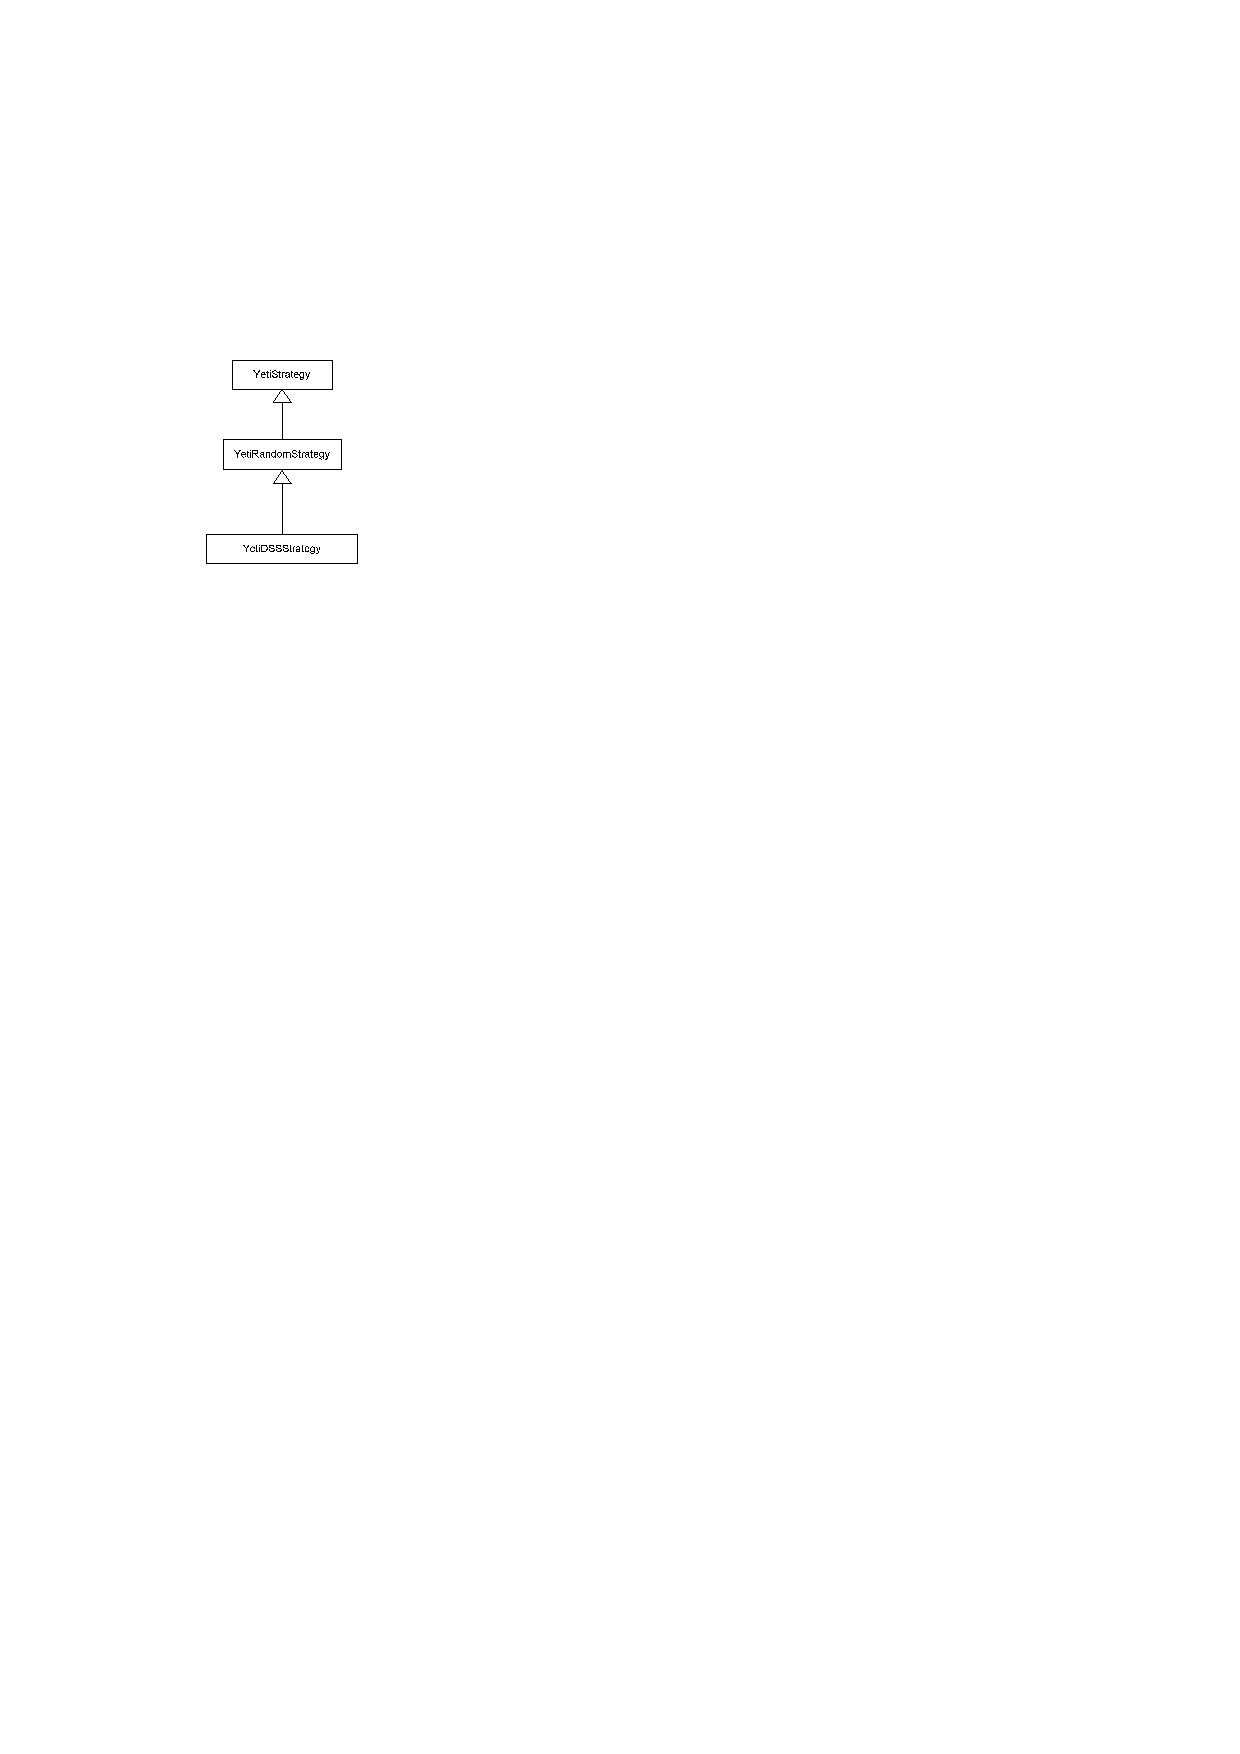
\includegraphics[width=4cm,height=5cm]{chapter4/hierarchy.pdf}
\caption{Class Hierarchy of DSSR in YETI}
\label{fig:hierarchyofDSSR}
\end{figure}





%%%%%%%%%%%%%%%%%    EVALUATION   %%%%%%%%%%%%%%%%%%%%


\section{Evaluation}\label{sec:eval}

The DSSR strategy is experimentally evaluated by comparing its performance with that of random and random+ strategy ~\cite{Leitner2007}. General factors such as system software and hardware, YETI specific factors like percentage of null values, percentage of newly created objects and interesting value injection probability have been kept constant in the experiments.

\subsection{Research questions}
For evaluating the DSSR strategy, the following research questions have been addressed in this study:
\begin{enumerate}
\item Is there an absolute best among R, R+ and DSSR strategies?
\item Are there classes for which any of the three strategies provide better results?
\item Can we pick the best default strategy between R, R+ and DSSR?
\end{enumerate}



\subsection{Experiments}

To evaluate the performance of DSSR we performed extensive testing of programs from the Qualitas Corpus~\cite{Tempero2010a}. The Qualitas Corpus is a curated collection of open source java projects built with the aim of helping empirical research on  software engineering. These projects have been collected in an organised form containing the source and binary forms. Version 20101126, which contains 106 open source java projects is used in the current evaluation. In our experiments we selected 60 random classes from 32 random projects. All the selected classes produced at least one fault and did not time out with maximum testing session of 10 minutes. Every class is tested thirty times by each strategy (R, R+, DSSR). Name, version and size of the projects to which the classes belong are given in table~\ref{table:projects} while test details of the classes is presented in table~\ref{table:Results}. Line of Code (LOC) tested per class and its total is shown in column 3 of table~\ref{table:Results}. 

Every class is evaluated through $10^5$ calls in each test session.\footnote{The total number of tests is thus $60\times 30\times 3 \times 10^5 = 540\times 10^6~tests$.} 
Because of the absence of the contracts and assertions in the code under test, similar approach as used in previous studies ~\cite{Oriol2012}, is followed using undeclared exceptions to compute unique failures.


\begin{table}[htp]
\caption{Name and versions of 32 Projects randomly selected from the Qualitas Corpus for the experiments}
\centering
\begin{tabular}{|r|l|r|r|}
\hline
{\textbf {S. No}}& 	{\textbf {Project Name}}	& 	{\textbf {Version}}		&	{\textbf {Size (MB)}}\\
\hline
1	&	apache-ant	&	1.8.1			&	59\\
2	&	antlr			&	3.2			&	13\\
3	&	aoi			&	2.8.1			&	35\\
4	&	argouml		&	0.30.2		&	112\\
5	&	artofillusion	&	281			&	5.4\\
6	&	aspectj		&	1.6.9			&	109.6\\
7	&	axion		&	1.0-M2		&	13.3\\
8	&	azureus		&	1			&	99.3\\
9	&	castor		&	1.3.1			&	63.2\\
10	&	cayenne		&	3.0.1			&	4.1\\
11	&	cobertura		&	1.9.4.1		&	26.5\\
12	&	colt			&	1.2.0			&	40\\
13	&	emma		&	2.0.5312		&	7.4\\
14	&	freecs		&	1.3.20100406	&	11.4\\
15	&	hibernate		&	3.6.0			&	733\\
16	&	hsqldb		&	2.0.0			&	53.9\\
17	&	itext			&	5.0.3			&	16.2\\
18	&	jasml		&	0.10			&	7.5 \\
19	&	jmoney		&	0.4.4			&	5.3\\
20	&	jruby			&	1.5.2			&	140.7\\
21	&	jsXe			&	04\_beta		&	19.9\\
22	&	quartz		&	1.8.3			&	20.4\\
23	&	sandmark		&	3.4			&	18.8\\
24	&	squirrel-sql	&	3.1.2			&	61.5\\
25	&	tapestry		&	5.1.0.5		&	69.2\\
26	&	tomcat		&	7.0.2			&	24.1\\
27	&	trove			&	2.1.0			&	18.2\\
28	&	velocity		&	1.6.4			&	27.1\\
29	&	weka		&	3.7.2			&	107\\
30	&	xalan		&	2.7.1			&	85.4\\
31	&	xerces		&	2.10.0		&	43.4\\
32	&	xmojo		&	5.0.0			&	15\\
\hline
\end{tabular}
\bigskip
\label{table:projects}
\end{table}



All tests are performed with a 64-bit Mac OS X Lion Version 10.7.4 running on 2 x 2.66 GHz 6-Core Intel Xeon processor with 6 GB (1333 MHz DDR3) of RAM. YETI runs on top of the Java\texttrademark  SE Runtime Environment [version 1.6.0\_35]. The machine took approximately 100 hours to process the experiments.


\subsection{Performance measurement criteria}
Various measures including the E-measure (expected number of failures detected), P-measure (probability of detecting at least one failure) and F-measure (number of test cases used to find the first fault) have been used by researchers to find the effectiveness of the random test strategy. The E-measure and P-measure have been heavily criticised~\cite{Chen2008} and are not considered effective measuring techniques while the F-measure has been often used by various researchers~\cite{Chen2004, Chen1996}. In our initial experiments the F-measure is used to evaluate the efficiency. However it was realised that this is not the right choice. In some experiments a strategy found the first fault quickly than the other but on completion of test session that very strategy found lower number of total faults than the rival strategy. The preference given to a strategy by F-measure because it finds the first fault quickly without giving due consideration to the total number of faults is not fair~\cite{Liu2012}.


  
The literature review revealed that the F-measure is used where testing stops after identification of the first fault and the system is given back to the developers to remove the fault. Currently automated testing tools test the whole system and print all discovered faults in one go therefore, F-measure is not the favourable choice. In our experiments, performance of the strategy is measured by the maximum number of faults detected in SUT by a particular number of test calls \cite{Ciupa2007, Ciupa2008b, Pacheco2007}. This measurement is effective because it considers the performance of the strategy when all other factors are kept constant.

%%%%%%%%%%%%%%%%%    RESULTS   %%%%%%%%%%%%%%%%%%%%
\begin{figure*}[ht]
\centering
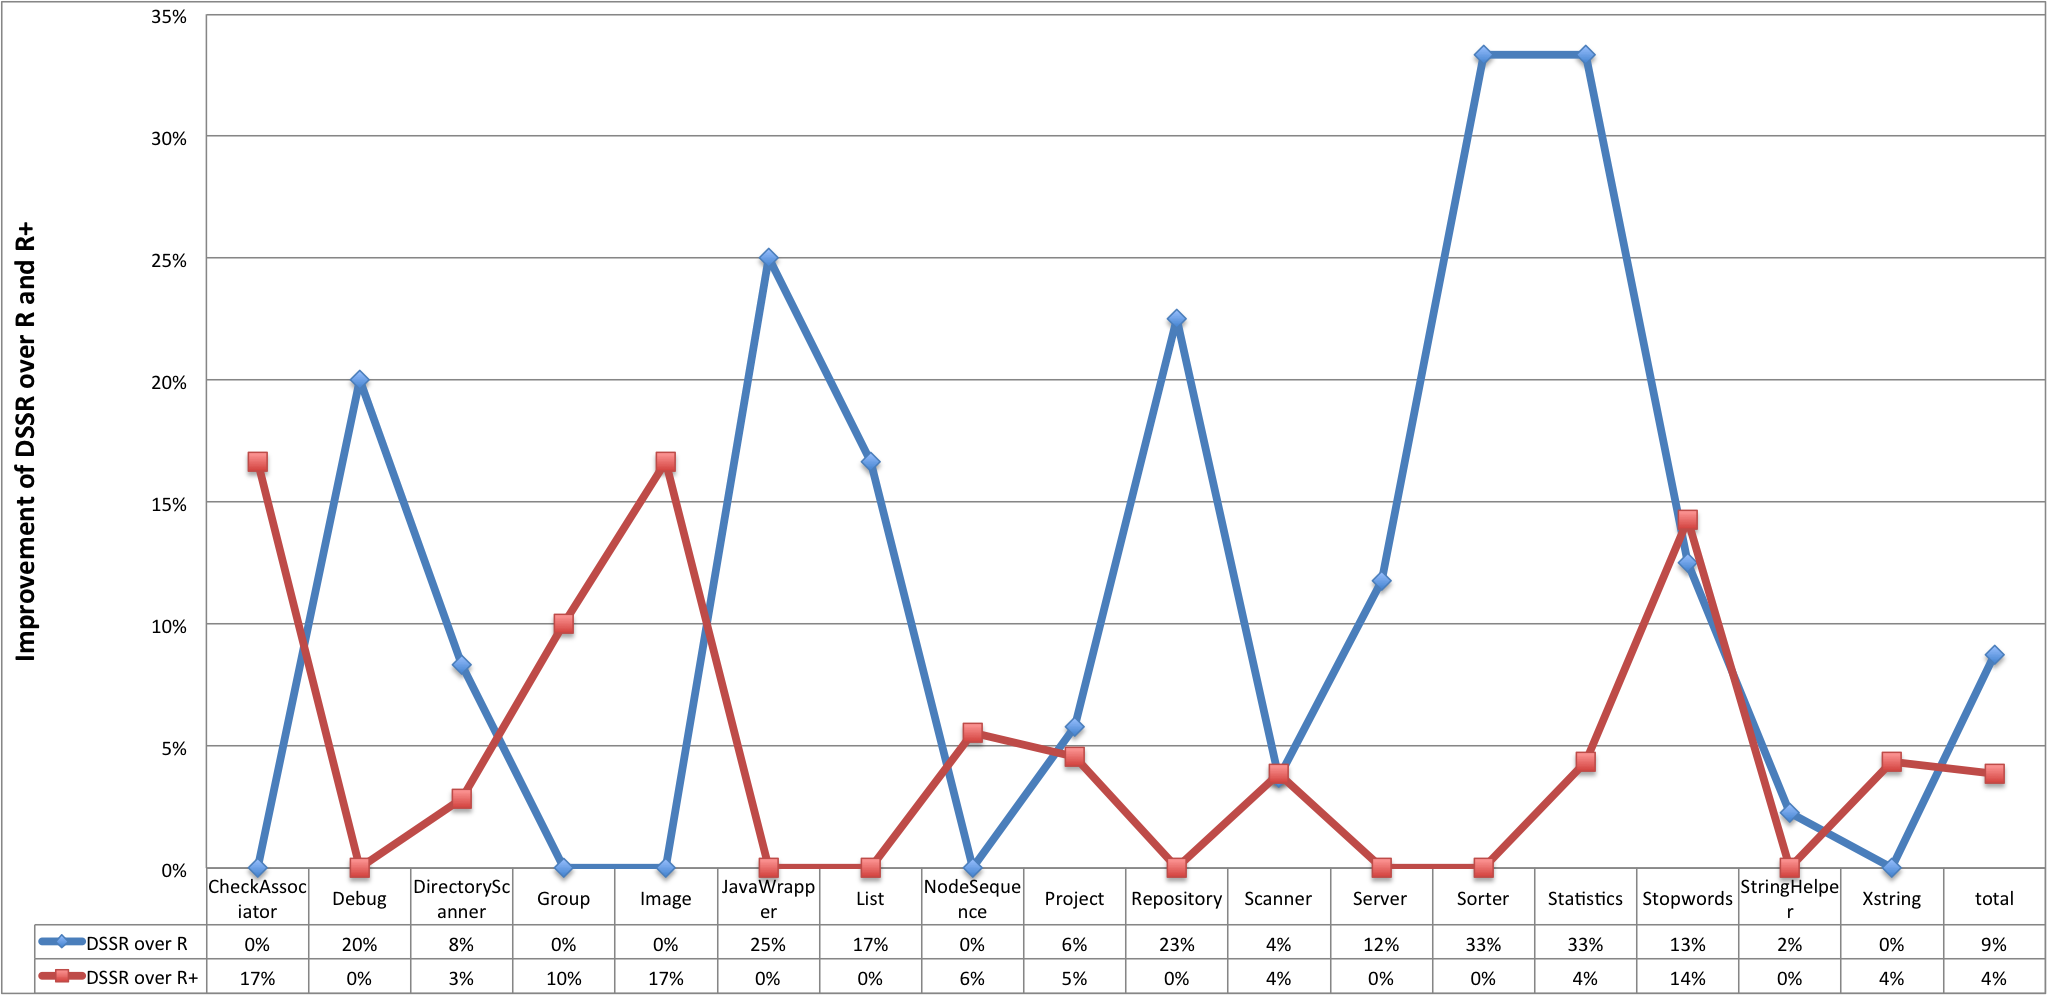
\includegraphics[width=14cm]{chapter4/DssrImprove.png}
\caption{Improvement of DSSR strategy over Random and Random+ strategy.}
\label{fig:LineChart}
\end{figure*}

%%%%%%%%%%%%%%%%%%%%%%%%%%%%%%%%%%%%%%%%%%%%



\begin{table*} [htp!]
  \scriptsize
 \caption{Experiments result presenting Serial Number (S.No), Class Name, Line of Code (LOC), mean, maximum and minimum number of faults and relative standard deviation for each Random (R), Random+ (R+) and Dirt Spot Sweeping Random (DSSR) strategies.}
	%\begin{minipage}[h]{\pagewidth}\centering
	\hspace{-2cm}
	\noindent\makebox[\textwidth]{
 	\begin{tabularx}{1 \textwidth}{r l r r r r r r r r r r r r r}
      %\aline

      \multirow{2}{*}{{\textbf {S. No}}}		& \multirow{2}{*}{{\textbf {Class Name}}}		& \multirow{2}{*}{{\textbf {LOC}}}	& \multicolumn{4}{c}{{\textbf {R}}}							&	\multicolumn{4}{c}{{\textbf {R+}}}							&	\multicolumn{4}{c}{{\textbf {DSSR}}}	\\
      %\cline{3-14} 
      						&						&			& Mean 	& Max	& Min 	& 	R-STD				& Mean 	& Max 	& Min 	&	 R-STD 			& Mean 		& Max 		& Min		& R-STD \\


1						& ActionTranslator			&709		& 96		&	96	&	96	& 	0					& 96		& 96 		& 96		& 		0			& 96			& 96			& 96			&	0\\     
2						& AjTypeImpl				&1180		& 80		&	83	&	79	& 	0.02					& 80		& 83 		& 79		& 		0.02			& 80			& 83			& 79			&	0.01\\      
\textbf{3}					& \textbf{Apriori}			&\textbf{292}	& \textbf{3}&	\textbf{4}	&\textbf{3}	& \textbf{0.10}			& \textbf{3}& \textbf{4} 		& \textbf{3}& \textbf{0.13}	& \textbf{3}	& \textbf{4}	& \textbf{3}	&\textbf{0.14}\\      
4						& BitSet					&575		& 9		&	9	&	9	& 	0					& 9		& 9 		& 9		& 		0			& 9			& 9			& 9			&	0\\       
5						& CatalogManager			&538		& 7		&	7	&	7	& 	0					& 7		& 7 		& 7		& 		0			& 7			& 7			& 7			&	0\\    
\textbf{6}					& \textbf{CheckAssociator}	&\textbf{351}	& \textbf{7}	&	\textbf{8}	&	\textbf{2}	& 	\textbf{0.16}					& \textbf{6}		& \textbf{9} 		& \textbf{2}		& 		\textbf{0.18}			& \textbf{7}			& \textbf{9}			& \textbf{6}			&	\textbf{0.73}\\    
\textbf{7}						& \textbf{Debug}					&\textbf{836}		& \textbf{4}		&	\textbf{6}	&	\textbf{4}	& 	\textbf{0.13}					& \textbf{5}		& \textbf{6} 		& \textbf{4}		& 		\textbf{0.12}			& \textbf{5}			& \textbf{8}			& \textbf{4}			&	\textbf{0.19}\\       
\textbf{8}						& \textbf{DirectoryScanner}			&\textbf{1714}		& \textbf{33}		&	\textbf{39}	&	\textbf{20}	& 	\textbf{0.10}					& \textbf{35}		& \textbf{38} 		& \textbf{31}		& 		\textbf{0.05}			& \textbf{36}			& \textbf{39}			& \textbf{32}			&	\textbf{0.04}\\      
9						& DiskIO					&220		& 4		&	4	&	4	& 	0					& 4		& 4 		& 4		& 		0			& 4			& 4			& 4			&	0\\      
10						& DOMParser				&92			& 7		&	7	&	3	& 	0.19					& 7		& 7 		& 3		& 		0.11			& 7			& 7			& 7			&	0\\      
11						& Entities					&328		& 3		&	3	&	3	& 	0					& 3		& 3 		& 3		& 		0			& 3			& 3			& 3			&	0\\      
12						& EntryDecoder			&675		& 8		&	9	&	7	& 	0.10					& 8		& 9 		& 7		& 		0.10			& 8			& 9			& 7			&	0.08\\   
13						& EntryComparator			&163		& 13		&	13	&	13	& 	0					& 13		& 13 		& 13		& 		0			& 13			& 13			& 13			&	0\\      
14						& Entry					&37			& 6		&	6	&	6	& 	0					& 6		& 6 		& 6		& 		0			& 6			& 6			& 6			&	0\\   
15						& Facade					&3301		& 3		&	3	&	3	& 	0					& 3		& 3 		& 3		& 		0			& 3			& 3			& 3			&	0\\   
16						& FileUtil					&83			& 1		&	1	&	1	& 	0					& 1		& 1 		& 1		& 		0			& 1			& 1			& 1			&	0\\      
17						& Font					&184		&12		&	12	&	11	& 	0.03					& 12		& 12 		& 11		& 		0.03			& 12			& 12			& 11			&	0.02\\        
18						& FPGrowth				&435		& 5		&	5	&	5	& 	0					& 5		&  5		& 5		& 		0			& 5			& 5			& 5			&	0	\\       
19						& Generator				&218		& 17		&	17	&	17	& 	0					& 17		& 17 		& 17		& 		0			& 17			& 17			& 17			&	0	\\      
\textbf{20}						& \textbf{Group}					&\textbf{88}			& \textbf{11}		&	\textbf{11}	&	\textbf{10}	& 	\textbf{0.02}					& \textbf{10}		& \textbf{4} 		& \textbf{11}		& 		\textbf{0.15}			& \textbf{11}			& \textbf{11}			& \textbf{11}			&	\textbf{0}	\\      
21						& HttpAuth				&221		& 2		&	2	&	2	& 	0					& 2		& 2 		& 2		& 		0			& 2			& 2			& 2			&	0	\\         
\textbf{22}						& \textbf{Image}					&\textbf{2146}		& \textbf{13}		&	\textbf{17}	&	\textbf{7}	& 	\textbf{0.15}					& \textbf{12}		& \textbf{14} 		& \textbf{4}	& 		\textbf{0.15}			& \textbf{14}			& \textbf{16}			& \textbf{11}			&	\textbf{0.07}\\        
23						& InstrumentTask			&71			& 2		&	2	&	1	& 	0.13					& 2		& 2 		& 1		& 		0.09			& 2			& 2			& 2			&	0	\\    
24						& IntStack					&313		& 4		&	4	&	4	& 	0					& 4		& 4 		& 4		& 		0			& 4			& 4			& 4			&	0	\\      
25						& ItemSet					&234		& 4		&	4	&	4	& 	0					& 4		& 4 		& 4		& 		0			& 4			& 4			& 4			&	0	\\       
26						& Itextpdf					&245		& 8		&	8	&	8	& 	0					& 8		&  8		& 8		& 		0			& 8			& 8			& 8			&	0\\      
\textbf{27}						& \textbf{JavaWrapper}				&\textbf{513}		&\textbf{3}		&	\textbf{2}	&	\textbf{2}	& 	\textbf{0.23}					& \textbf{4}		& \textbf{4} 		& \textbf{3}		& 		\textbf{0.06}			& \textbf{4}			& \textbf{4}			& \textbf{3}			&	\textbf{0.05}\\      
28						& JmxUtilities				&645		& 8		&	8	&	6	& 	0.07					& 8		& 8 		& 7		& 		0.04			& 8			& 8			& 7			&	0.04\\      
\textbf{29}						& \textbf{List}					&\textbf{1718}		& \textbf{5}		&	\textbf{6}	&	\textbf{4}	& 	\textbf{0.11}					& \textbf{6}		& \textbf{6} 		& \textbf{4}		& 		\textbf{0.10}			&\textbf{6}			& \textbf{6}			& \textbf{5}			&	\textbf{0.09}\\      
30						& NameEntry				&172		& 4		&	4	&	4	& 	0					& 4		& 4 		& 4		& 		0			& 4			& 4			& 4			&	0	\\  
\textbf{31}						& \textbf{NodeSequence}			&\textbf{68}			& \textbf{38}		&	\textbf{46}	&	\textbf{30}	& 	\textbf{0.10}					& \textbf{36}		& \textbf{45} 		& \textbf{30}		& 		\textbf{0.12}			& \textbf{38}			& \textbf{45}			& \textbf{30}			&	\textbf{0.08}	\\     
32						& NodeSet				&208		& 28		&	29	&	26	& 	0.03					& 28		& 29 		& 26		& 		0.04			& 28			& 29			& 26			&	0.03	\\  
33						& PersistentBag			&571		& 68		&	68	&	68	& 	0					& 68		&  68		& 68		& 		0			& 68			& 68			& 68			&	0	\\         
34						& PersistentList				&602		& 65		&	65	&	65	& 	0					& 65		&  65		& 65		& 		0			& 65			& 65			& 65			&	0	\\    
35						& PersistentSet				&162		& 36		&	36	&	36	& 	0					& 36		&  36		& 36		& 		0			& 36			& 36			& 36 			&	0	\\        
\textbf{36}						& \textbf{Project}					&\textbf{470}		& \textbf{65}		&	\textbf{71}	&	\textbf{60}	& 	\textbf{0.04}					& \textbf{66}		&  \textbf{78}		& \textbf{62}		& 		\textbf{0.04}			& \textbf{69}			& \textbf{78}			& \textbf{64}			&	\textbf{0.05}	\\        
\textbf{37}						& \textbf{Repository}				&\textbf{63}			& \textbf{31}		&	\textbf{31}	&	\textbf{31}	& 	\textbf{0}					& \textbf{40}		&  \textbf{40}		& \textbf{40}		& 		\textbf{0}			& \textbf{40}			& \textbf{40}			& \textbf{40}			&	\textbf{0}	\\         
38						& Routine					&1069		& 7		&	7	&	7	& 	0					& 7		&  7		& 7		& 		0			& 7			& 7			& 7			&	0	\\
39						& RubyBigDecimal			&1564		& 4 		&	4	&	4	& 	0					& 4		& 4 		& 4		& 		0			& 4			& 4			& 4			&	0\\      
40						& Scanner				&94			& 3		&	5	&	2	& 	0.20					& 3		& 5 		& 2		& 		0.27			& 3			& 5			& 2			&	0.25\\      
\textbf{41}						& \textbf{Scene}					&\textbf{1603}		& \textbf{26}		&	\textbf{27}	&	\textbf{26}	& 	\textbf{0.02}					& \textbf{26}		& \textbf{27} 		& \textbf{26}		& 		\textbf{0.02}			& \textbf{27}			& \textbf{27}			& \textbf{26}			&	\textbf{0.01}\\      
42						& SelectionManager			&431		& 3		&	3	&	3	& 	0					& 3		& 3 		& 3		& 		0			& 3			& 3			& 3			&	0\\      
\textbf{43}						& \textbf{Server}					&\textbf{279}		&\textbf{15}		&	\textbf{21}	&	\textbf{11}	& 	\textbf{0.20}					& \textbf{17}		& \textbf{21} 		& \textbf{12}		& 		\textbf{0.16}			& \textbf{17}			& \textbf{21}			& \textbf{12}			&	\textbf{0.14}\\      
\textbf{44}						& \textbf{Sorter}					&\textbf{47}			& \textbf{2}		&	\textbf{2}	&	\textbf{1}	& 	\textbf{0.09}					& \textbf{3}		& \textbf{3} 		& \textbf{2}		& 		\textbf{0.06}			&\textbf{3}			& \textbf{3}			& \textbf{3}			&	\textbf{0}\\      
45						& Sorting					&762		& 3		&	3	&	3	& 	0					& 3		& 3 		& 3		& 		0			& 3			& 3			& 3			&	0\\      
\textbf{46}						& \textbf{Statistics}				&\textbf{491}		& \textbf{16}		&	\textbf{17}	&	\textbf{12}	&	\textbf{0.08}					& \textbf{23}		& \textbf{25} 		& \textbf{22}		& 		\textbf{0.03}			& \textbf{24}			& \textbf{25}			& \textbf{22}			&	\textbf{0.04}\\      
47						& Status					&32			& 53		&	53	&	53	& 	0					& 53		& 53 		& 53		& 		0			& 53			& 53			& 53			&	0\\      
\textbf{48}						& \textbf{Stopwords}				&\textbf{332}		& \textbf{7}		&	\textbf{8}	&	\textbf{7}	& 	\textbf{0.03}					& \textbf{7}		&  \textbf{8}		& \textbf{6}		& 		\textbf{0.08}			& \textbf{8}			& \textbf{8}			& \textbf{7}			&	\textbf{0.06}\\      
\textbf{49}						& \textbf{StringHelper}				&\textbf{178}		& \textbf{43}	 	& 	\textbf{45}	&	\textbf{40}	& 	\textbf{0.02}					& \textbf{44}		&  \textbf{46}		& \textbf{42}		& 		\textbf{0.02}			& \textbf{44}			& \textbf{45}			& \textbf{42}			&	\textbf{0.02}\\      
50						& StringUtils				&119		& 19 		&	19	&	19	& 	0					& 19		& 19 		& 19		& 		0			& 19			& 19			& 19			&	0\\      
51						& TouchCollector			&222		& 3		&	3	&	3	& 	0					& 3		&  3		& 3		& 		0			& 3			& 3			& 3			&	0\\      
52						& Trie					&460		& 21		&	22	&	21	& 	0.02					& 21		&  22		& 21		& 		0.01			& 21			& 22			& 21			&	0.01\\      
53						& URI					&3970		& 5 		&	5	&	5	& 	0					& 5		&  5		& 5		& 		0			& 5			& 5			& 5			&	0\\      
54						& WebMacro				&311		& 5		&	5	&	5	& 	0					& 5		&  6		& 5		& 		0.14			& 5			& 7			& 5			&	0.28\\      
55						& XMLAttributesImpl			&277		& 8		&	8	&	8	& 	0					& 8		&  8		& 8		& 		0			& 8			& 8			& 8			&	0\\      
56						& XMLChar				&1031		& 13		&	13	&	13	& 	0					& 13		&  13		& 13		& 		0			& 13			& 13			& 13			&	0\\      
57						& XMLEntityManger			&763		& 17		&	18	&	17	& 	0.01					& 17		&  17		& 16		& 		0.01			& 17			& 17			& 17			&	0\\      
58						& XMLEntityScanner			&445		& 12		&	12	&	12	& 	0					& 12		&  12		& 12		& 		0			& 12			& 12			& 12			&	0\\      
59						& XObject					&318		& 19		&	19	&	19	& 	0					& 19		&  19		& 19		& 		0			& 19			& 19			& 19			&	0\\      
\textbf{60}						& \textbf{XString}					&\textbf{546}		& \textbf{23}		&	\textbf{24}	&	\textbf{21}	& 	\textbf{0.04}					& \textbf{23}		&  \textbf{24}		& \textbf{23}		& 		\textbf{0.02}			& \textbf{24}			& \textbf{24}			& \textbf{23}			&	\textbf{0.02}\\      

    						\multicolumn{2}{c}{\textbf{Total}}	&35,785	&1040	&	1075	&    973	&	2.42				& 1061	&1106	&1009	&		2.35		& 1075		& 1118		& 1032		& 	1.82\\
   %\hline
     \end{tabularx} }
 	%\end{minipage}
    \bigskip
    \label{table:Results}
\end{table*}

\section{Results}\label{sec:res}
Results of the experiments including class name, Line of Code (LOC), mean value, maximum and minimum number of unique failures and relative standard deviation for each of the 60 classes tested using R, R+ and DSSR strategy are presented in Table~\ref{table:Results}. Each strategy found an equal number of faults in 31 classes while in the remaining 29 classes the three strategies performed differently from one another. The total of mean values of unique failures in DSSR (1075) is higher than for R (1040) or R+ (1061) strategies. 
%Results given in Table~\ref{table:ttest} can be split into three different categories as shown in Table~\ref{table:categories}. 
DSSR also finds a higher number of maximum unique failures (1118) than both R (1075), and R+ (1106). DSSR strategy finds 43 and 12 more unique faults compared to R and R+ respectively. The minimum number of unique faults found by DSSR (1032) is also higher than for R (973) and R+ (1009) which attributes to higher efficiency of DSSR strategy over R and R+ strategies. 

% How to write relative standard deviation.
% Eventually, the standard deviations are all of the order of magnitude of .1\% for all strategies.

\subsection{Is there an absolute best among R, R+ and DSSR strategies?}
Based on our findings DSSR is at least as good as R and R+ in almost all cases, it is also significantly better than both R and R+ in 12\% of the classes. Figure~\ref{fig:LineChart} presents the average improvements of DSSR strategy over R and R+ strategy over the 17 classes for which there is a significant difference between DSSR and R or R+. The blue line with diamond symbol shows performance of DSSR over R and the red line with square symbols depicts the improvement of DSSR over R+ strategy. The classes where blue line with diamond symbols show the improvement of DSSR over R and red line with square symbols show the improvement of DSSR over R+. 

The improvement of DSSR over R and R+ strategy is calculated by applying the formula (1) and (2) respectively.

\begin{equation} \frac{Averagefaults_{(DSSR)} - Averagefaults_{(R)}}{Averagefaults_{(R)}} * 100  \end{equation}

\begin{equation} \frac{Averagefaults_{(DSSR)} - Averagefaults_{(R+)}}{Averagefaults_{(R+)}}  * 100 \end{equation}

The findings show that DSSR strategy perform up to 33\% better than R and up to 17\% better than R+ strategy. In some cases DSSR perform equally well with R and R+ but in no case DSSR performed lower than R and R+. Based on the results it can be stated that DSSR strategy is a better choice than R and R+ strategy. 

\begin{table*}[htp]
\small
\caption{T-test results of the classes}
\smallskip
\centering
\begin{tabular}{rlrrrl}
\hline
 \multirow{2}{*} {{\textbf {S. No}}}	& \multirow{2}{*}{{\textbf {Class Name}}}	&  \multicolumn{3}{c}{{\textbf {T-test Results}}} & \multirow{2}{*}{{\textbf {Interpretation}}} \\

		&					& 	DSSR, R			& DSSR, R+	&  R, R+ 		& 		\\
\hline
1		&	AjTypeImpl		&	1 				& 1 			& 1			& 		\\	
2		&	Apriori			&	\textbf{0.03}	 	& 0.49		& 0.16		&		\\	
3		&	CheckAssociator	&	\textbf{0.04}	 	& \textbf{0.05}	& 0.44		& DSSR better		\\	
4		&	Debug			&	\textbf{0.03}	 	& 0.14		& 0.56		&		\\	
5		&	DirectoryScanner	&	\textbf{0.04}	 	& \textbf{0.01}	& 0.43		& DSSR better		\\
6		&	DomParser		&	\textbf{0.05}	 	& 0.23		& 0.13		&				\\
7		&	EntityDecoder		&	\textbf{0.04}	 	& 0.28		& 0.3			&		\\			
8		&	Font				&	0.18	 			& 0.18		& 1			&		\\
9		&	Group			&	0.33	 			& \textbf{0.03}	& \textbf{0.04}	& DSSR = R \textgreater R+	\\
10		&	Image			&	\textbf{0.03}		& \textbf{0.01}	& 0.61		& DSSR better \\		
11		&	InstrumentTask		&	0.16				& 0.33		& 0.57		& \\
12		&	JavaWrapper		&	\textbf{0.001}		& 0.57		& 0.004		& DSSR = R+ \textgreater R \\
13		& 	JmxUtilities		&	0.13				& 0.71		& 0.08		&	\\
14		&	List				& 	\textbf{0.01}		&0.25		&\textbf{0}		& DSSR = R+ \textgreater R \\
15		&	NodeSequence	&	0.97				&\textbf{0.04}	&\textbf{0.06}	& DSSR = R \textgreater R+ \\
16		&	NodeSet			&	\textbf{0.03}		&0.42		&0.26		& 	\\
17		&	Project			&	\textbf{0.001}		&0.57		&\textbf{0.004}	& DSSR better \\		
18		&	Repository		&	\textbf{0}			&1			&\textbf{0}		& DSSR = R+ \textgreater R \\
19		&	Scanner			&	1				&\textbf{0.03}	&\textbf{0.01}	& DSSR better \\
20		&	Scene			&	\textbf{0}			&\textbf{0}		& 1			& DSSR better \\
21		&	Server			&	\textbf{0.03}		& 0.88		&\textbf{0.03} 	& DSSR = R+ \textgreater R \\
22		&	Sorter			& 	\textbf{0}			& 0.33		&\textbf{0}		& DSSR = R+ \textgreater R \\
23		&	Statistics			&	\textbf{0}			& 0.43		&\textbf{0}		& DSSR = R+ \textgreater R\\
24		&	Stopwords		&	\textbf{0}			& 0.23		&\textbf{0}		& DSSR = R+ \textgreater R \\
25		&	StringHelper		&	\textbf{0.03}		& 0.44		&0.44		& DSSR = R+ \textgreater R\\
26		& 	Trie				&	0.1				& 0.33		&0.47		& DSSR better \\
27		&	WebMacro		&	0.33				& 1			&0.16		& \\
28		&	XMLEntityManager	&	0.33				& 0.33		&0.16		& \\
29 		&	XString			&	0.14				&\textbf{0.03}	&0.86		& \\


\end{tabular}
\bigskip
\label{table:ttest}
\end{table*}

\subsection{Are there classes for which any of the three strategies provide better results?}


T-tests applied to the data given in Table~\ref{table:ttest} show that DSSR is significantly better in 7 classes from R and R+ strategy, in 8 classes DSSR performed similarly to R+  but significantly higher than R, and in 2 classes DSSR performed similarly to R but significantly higher than R+. There is no case R and R+ strategy performed significantly better than DSSR strategy. Expressed in percentage: 72\%  of the classes do not show significantly different behaviours whereas in 28\% of hte classes, the DSSR strategy performs significantly better than at least one of R and R+. It is interesting to note that in no single case R and R+ strategies performed better than DSSR strategy. We attribute this to DSSR possessing the qualities of R and R+ whereas containing the spot sweeping feature.


%Results of the 60 classes tested in the study are divided in to 11 different categories as presented in ~\ref{table:categories}. 
\begin{comment}
\begin{table}[h]
\caption{Results of the 60 classes are divided into 11 categories}
\centering
\begin{tabular}{|r|l|r|}
\hline
{\textbf {S. No}}	& 	{\textbf {Category}}			& 	{\textbf {Result}}\\
\hline
1		&	DSSR > R			&	12 \\	
2		&	DSSR > R+		&	10 \\	
3		&	DSSR = R			&	5 \\	
4		&	DSSR = R+		&	7 \\	
5		&	R+ > R 			&	10 \\	
6		&	R+ < R			&	5 \\	
7		&	R+ = R			&	2 \\	
8		&	R > R+			&	4 \\
9		&	DSSR < R			&	0 \\	
10		&	DSSR < R+		&	0 \\
11		&	DSSR = R = R+	&	43 \\			
\hline
\end{tabular}
\bigskip
\label{table:categories}
\end{table}

% pie chart is removed because the length of the paper is exceeding 10 pages and also it don't make much sense i believe.
%\begin{figure}[h]
%\centering
%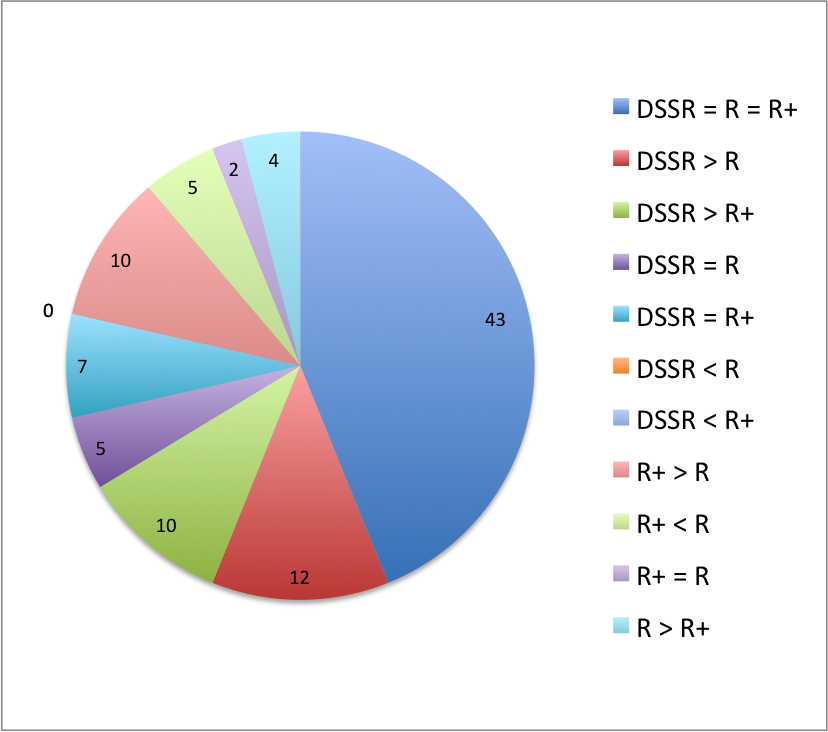
\includegraphics[width=8cm,height=7cm]{pie5.png}
%\caption{Division of result in to categories}
%\label{fig:pie}
%\end{figure}






The first category contain 12 classes where DSSR strategy performs better than R. 
The second category contain 10 classes where DSSR strategy performs better than R+. 
The third category contain 5 classes where DSSR strategy and R performs equally well.
The fourth category contain 7 classes where DSSR and R+ performs equally well. 
The fifth category contain 10 classes where R+ performs better than R.
The sixth category contain 5 classes where R performs better than R+.
The seventh category contain 2 classes where R and R+ performs equally well.
The eighth category contain 4 classes where R performs better than R+.
Category 9 and 10 shows that neither R nor R+ performed better than DSSR strategy.
The last category shows each strategy performing equally well for 43 classes. Expressing in percentage, 72\% classes do not show different behaviours whereas in 28\% of classes, the DSSR strategy performs better than R and R+ strategy. It is interesting to note that in no single case R and R+ strategies performed better than DSSR strategy. This is attributed to the fact that DSSR strategy possess the qualities of R and R+ and has the additional advantage of spot sweeping.

\end{comment}

\subsection{Can we pick the best default strategy between R, R+ and DSSR?}

Analysis of the experimental data reveal that DSSR strategy has an edge over R and R+. This is because of the additional feature of Spot Sweeping in DSSR strategy.

In spite of the better performance of DSSR strategy compared to R and R+ strategies the present study does not provide ample evidence to pick it as the best default strategy because of the overhead induced by this strategy (see next section). Further study might give conclusive evidence. 




%%%%%%%%%%%%%%%%%    DISCUSSION   %%%%%%%%%%%%%%%%%%%%

\section{Discussion}\label{sec:discussion3}
In this section we discuss various factors such as the time taken, effect of test duration, number of tests, number of faults in the different strategies and the effect of finding first fault in the DSSR strategy.

\textbf{Time taken to execute an equal number of test cases:}
The DSSR strategy takes slightly more time (up to 5\%) than both pure random and random plus which may be due to maintaining sets of interesting values during the execution. We do not believe that the overhead can be reduced. 

\textbf{Effect of test duration and number of tests on the results:}
All three techniques have the same potential for finding failures. If testing is continued for a long duration then all three strategies will find the same number of unique failures and the results will converge. We suspect however that some of the unique failures will take an extremely long time to be found by using random or random+ only. Further experiments should confirm this point.


\textbf{Effect of number of faults on results:} 
We found that the DSSR strategy performs better when the number of faults is higher in the code. The reason seems to be that when there are more faults, their domains are more connected and DSSR strategy works better. Further studies might use historical data to pick the best strategy.

\textbf{Dependence of DSSR strategy to find the first unique failure early enough:}
During the experiments we noticed that if a unique failure is not found  quickly enough, there is no value added to the list of interesting values and then the test becomes equivalent to random+ testing. This means that better ways of populating failure-inducing values are needed for sufficient leverage to DSSR strategy. As an example, the following piece of code would be unlikely to fail under the current setting:

\begin{lstlisting}
public void test(float value){
 if(value == 34.4445)   10/0;
}
\end{lstlisting}

In this case, we could add constant literals from the SUT to the list of interesting values in a dynamic fashion. These literals can be obtained from the constant pool in the class files of the SUT.

In the example above the value 34.4445 and its surrounding values would  be added to the list of interesting values before the test starts and the DSSR strategy would find the unique failure right away.

\textbf{DSSR strategy and coverage:} Random strategies typically achieve high level of coverage~\cite{Oriol2010}. It might also be interesting to compare R, R+ and DSSR with respect to the achieved coverage or even to use a DSSR variant that adds a new interesting value and its neighbours when a new branch is reached.


\textbf{Threats to validity:} As usual with such empirical studies, the present work might suffer from a non-representative selection of classes. The selection in the current study is however made through random process and objective criteria, therefore, it seems likely that it would be representative. The parameters of the study might also have prompted incorrect results. But this is unlikely due to previous results on random testing~\cite{Oriol2012}.



%%%%%%%%%%%%%%%%%    RW   %%%%%%%%%%%%%%%%%%%%

\section{Related Work}\label{sec:rw}

Random testing is a popular technique with simple algorithm but proven to find subtle faults in complex programs and Java libraries~\cite{Csallner2004, Claessen2000, Pacheco2005}. Its simplicity, ease of implementation and efficiency in generating test cases make it the best choice for test automation~\cite{hamlet1994}. Some of the well known automated tools based on random strategy includes Jartege~\cite{Oriat2004}, Eclat~\cite{Pacheco2005}, JCrasher~\cite{Csallner2004}, AutoTest \cite{Ciupa2007, Ciupa2008a} and YETI~\cite{Oriol2012, Oriol2010}.

In pursuit of better test results and lower overhead, many variations of random strategy have been proposed~\cite{Chan2002, Chen2003, Chen2010, Chen2005, Chen2004a}. Adaptive random testing (ART), Quasi-random testing (QRT) and Restricted Random testing (RRT) achieved better results by selecting test inputs randomly but evenly spread across the input domain. Mirror ART and ART through dynamic partitioning increased the performance by reducing the overhead of ART. The main reason behind better performance of the strategies is that even spread of test input increases the chance of exploring the fault patterns present in the input domain.

A more recent research study \cite{Yoo2012} stresses on the effectiveness of data regeneration in close vicinity of the existing test data. Their findings showed up to two orders of magnitude more efficient test data generation than the existing techniques. Two major limitations of their study are the requirement of existing test cases to regenerate new test cases, and increased overhead due to ``meta heuristics search'' based on hill climbing algorithm to regenerate new data. In DSSR no pre-existing test cases are required because it utilises the border values from R+ and regenerate the data very cheaply in a dynamic fashion different for each class under test without any prior test data and with comparatively lower overhead. 
  
The random+ (R+) strategy is an extension of the random strategy in which interesting values, beside pure random values, are added to the list of test inputs~\cite{Leitner2007}. These interesting values includes border values which have high tendency of finding faults in the given SUT~\cite{Beizer1990}. Results obtained with R+ strategy show significant improvement over random strategy~\cite{Leitner2007}. DSSR strategy is an extension of R+ strategy which starts testing as R+ until a fault is found then it switches to spot sweeping.

%It is interesting that numerous efforts have been made to discover the fault patterns~\cite{Chen2010, Chen2005, Chan2002, Chen2004a, Chen2003}, etc. but in our knowledge, none has been published on covering/sweeping all the faults lying in a specific pattern once it has been discovered.


A common practice to evaluate performance of an extended strategy is to compare the results obtained by applying the new and existing strategy to identical programs~\cite{Duran1984, Gutjahr1999, hamlet1990}. Arcuri et al. \cite{Arcuri2012}, stress on the use of random testing as a baseline for comparison with other test strategies. We followed the procedure and evaluated DSSR strategy against R and R+ strategies under identical conditions.

In our experiments we selected projects from the Qualitas Corpus~\cite{Tempero2010} which is a collection of open source java programs maintained for independent empirical research. The projects in Qualitas Corpus are carefully selected that spans across the whole set of java applications~\cite{Oriol2012, Tempero2008,  Tempero2010a}.


%%%%%%%%%%%%%%%%%    CONCLUSIONS   %%%%%%%%%%%%%%%%%%%%


\section{Conclusions}\label{sec:conc}
The main goal of the present study was to develop a new random strategy which could find more faults in lower number of test cases. We developed a new strategy named. ``DSSR strategy'' as an extension of R+, based on the assumption that in a significant number of classes, failure domains are contiguous or located closely. The DSS strategy, a strategy which adds neighbouring values of the failure finding value to a list of interesting values, was implemented in the random testing tool YETI to test 60 classes, 30 times each, from Qualitas Corpus with each of the 3 strategies R, R+ and DSSR. The newly developed DSSR strategy uncovers more unique failures than both random and random+ strategies with a 5\% overhead. We found out that for 7 (12\%) classes DSSR was significantly better than both R+ and R, for 8 (13\%) classes DSSR performed similarly to R+ and significantly better than R, while in 2 (3\%) cases DSSR performed similarly to R and significantly better than R+. In all other cases, DSSR, R+ and R do not seem to perform significantly differently. Overall, DSSR yields encouraging results and advocates to develop the technique further for settings in which it is significantly better than both R and R+ strategies.



\externaldocument{chapter5}
\chapter{Automated Discovery of Failure Domain}
\label{chap:ADFD}
%\ifpdf
%    \graphicspath{{chapter4/AdfdFigs/PNG/}{chapter4/AdfdFigs/PDF/}{chapter4/AdfdFigs/}}
%\else
 %   \graphicspath{{chapter4/AdfdFigs/EPS/}{chapter4/AdfdFigs/}}
%\fi

\section{Introduction}\label{sec:intro5}
Testing is a fundamental requirement for assessing the quality of any software. Manual testing is labour-intensive and error-prone; therefore, automated testing is often used which significantly reduces the cost of software development and its maintenance~\cite{beizer1995black}. Most of the modern black-box testing techniques execute the Software Under Test (SUT) with specific input and results obtained are compared against the test oracle. A report is generated at the end of each test session depicting any discovered faults and the input values which triggers the failures. Developers fix the discovered faults in the SUT with the help of these reports. The revised version of the system is given back to the testers to find more faults and this process continues till the desired level of quality already set in the test plan is achieved or the provided resources are exhausted~\cite{parnin2011automated}.

%The fact that exhaustive testing for any non-trivial program is not possible compels the testers to come up with some strategy of input selection from the whole input domain. Random is one of the possible strategies widely used in automated tools. It is intuitively simple and easy to implement~\cite{ciupa2008finding, miller2006empirical}. It involves a minimum or no overhead in input selection and lacks human bias~\cite{hamlet1994random, linger1993cleanroom}. Random testing has several benefits, but there are some limitations as well, including low code coverage~\cite{offutt1996semantic} and discovery of lower number of faults~\cite{Chen1994}. To overcome these limitations and retain the benefits intact many researchers have successfully refined random testing. Adaptive Random Testing (ART) is one of the most significant refined version of random testing. Experiments performed using ART showed up to 50\% better results compared to the traditional random testing ~\cite{chen2005adaptive}.  Similarly Restricted Random Testing (RRT)~\cite{chan2006restricted}, Mirror Adaptive Random Testing (MART) ~\cite{chen2004mirror}, Adaptive random testing for object oriented program (Artoo)~\cite{ciupa2008artoo}, Directed Adaptive Random Testing (DART) ~\cite{godefroid2005dart}, Lattice-based Adaptive Random Testing (LART)~\cite{mayer2005lattice} and Feedback-directed Random Testing (FDRT)~\cite{pacheco2007randoop, pacheco2007feedback} are some of the improved versions of random testing.

%All the above-mentioned versions of random testing are based on the observation of Chan et al.~\cite{chan1996proportional} that failure causing inputs across the whole input domain form certain kinds of domains. They classified these domains into point, block \& strip failure domain and suggested that the failure finding ability of testing could be improved by taking into consideration these failure domains (see Section~\ref{sec:failuredomains_2}). %In Section~\ref{sec:failuredomains_2} the square boxes represent the whole input domain. The black points, block and strip inside the boxes represent the faulty values while the white area inside the boxes represent legitimate values for a specific system. 

%\begin{figure}[h]
%\centering
%\includegraphics[width=14cm,height=5cm]{chapter5/ART_Patterns.png}
%\caption{Failure domains across input domain~\cite{chan1996proportional}}
%\label{fig:patterns}
%\end{figure}


% It is important to note that these techniques only identify a single instance of failure and do not  focus on the failure domain. 

%2.	It is also noticed that further analysis of fault lead to new faults which the testing process may not have identified.
%3. 	Experiments can be performed to analyse the frequency of existence of point, block and strip domain across the input domain. 

%Random testing is a black-box testing technique in which parts (methods/modules) of SUT are selected randomly and then executed against randomly generated test data from the whole input domain. Results obtained from the execution are either compared to the specifications of the SUT or language exceptions which served as a test oracle. Any test output that fail to meet the oracle either because of failing to comply the specification or trigger the exceptions are considered as potential faults. In this paper we present a new tool, called Automated Discovery of Failure Domain (ADFD), based on a random testing tool called York Extensible Testing Infrastructure (YETI), for not only finding fault but also its domain. ADFD utilise YETI to discover the fault in the given SUT and then generate a dynamic code for finding its domain. The found domain -- point, block or strip are presented on the graph at the end of each test session


%ADFD has been designed to decrease the time of system testing. Knowing the domain of the fault the debuggers This research can decrease the overall testing time by reducing the number of code exchanges between testers and debugger. It is achieved by tracking the failure domain and not only a single instance failure. Tracking failure domain provide more information about the behaviour of the fault.

%that also served as regression testing. None of the testing techniques evaluate the nature of the fault and the pattern in which the fault reside. 


%The aim of this research study is to find not only find the values for which the system fails but also the domains of failure causing inputs which will help in automated generation of fault targeted test cases for any black-box testing technique.\\


%Over the past few years there is a tremendous growth in development of hardware whose main focus is to increase the computer processing power. The computers that served as a mini and mainframe computers few years ago are turned into personal computer in todays modern age. To utilise this processing power various software development companies started to develop more sophisticated and processing hungry softwares. These softwares provide simple and easy to use Graphical User Interface (GUI) but on the back end they are equally complex and consist of thousands of instructions. This increase in size of the software also increases the difficulty of preserving high quality, reliability, portability, maintainability and efficiency of the software. These problems are mainly cater by software testing. The increase of complexity and size of softwares also forced the researchers to find new ways of software testing that are more efficient, reliable and speedy to cope with the ever increasing hardware and software industry.\\

%Mirror Adaptive Random Testing (MART) ~\cite{Chen2003}, Feedback-directed Random Testing (FDRT)~\cite{Pacheco2007}, Restricted Random Testing (RRT)~\cite{Chan2002} and Quasi Random Testing  (QRT)~\cite{Chen2005} are the strategies based on the same principle that found better results compared to ordinary random testing.

The Adaptive Random Testing (ART)~\cite{chen2005adaptive}, Restricted Random Testing (RRT)~\cite{chan2006restricted}, Mirror Adaptive Random Testing (MART) ~\cite{chen2004mirror}, Adaptive random testing for object oriented software (ARTOO)~\cite{ciupa2008artoo}, Directed Automated Random Testing (DART) ~\cite{godefroid2005dart}, Lattice-based Adaptive Random Testing (LART)~\cite{mayer2005lattice} and Feedback-directed Random Testing (FDRT)~\cite{pacheco2007randoop, pacheco2007feedback} are few of the improved versions of random testing based on the existence of contiguous failure domains within the input domain (see Section~\ref{sec:failuredomains_2} for more details on failure domains). All these techniques try to detect a single instance of failure ignoring the underlying failure domain. It is interesting that, in our knowledge, no specific strategy has been developed to evaluate the failure domains. This chapter describes a new test strategy called Automated Discovery of Failure Domain (ADFD), which not only finds the failure and failure domains but also present the pass and fail domains graphically. The idea of identification of pass and fail domain is attractive because it provides an insight of the domains in the given SUT. Some important aspects of ADFD strategy presented in the chapter include:

\begin{itemize}
\item Description and implementation of the new ADFD strategy in YETI.
\item Evaluation to assess ADFD strategy by testing classes with different failure domains.
\item Reduction in test duration by identification of all failure domains instead of a single instance of failure.
\item Improvement in test efficiency by helping debugger to consider all failure occurrences during debugging. 
\end{itemize}


% Additionally, ADFD test strategy can also be used to identify frequency of point, block and strip fault domain across the production softwares.



%The main objective behind ADFD is to get an automated frame work that find the existence of fault and fault domain across the input domain, decrease debugging time and to discover any more faults missed by the testing system. Significant research has been done to utilise the failure domains but their existence, nature and boundaries need further attention. Having fault domain information prior to testing enables the tester to guide testing according to the failure domain of the SUT, for example pure random testing is more effective for point domain than block and strip domains where as ART, MART, FDRT, RRT and QRT are more effective for block and strip fault domains than point fault domain.

%In our previous research we extended the same idea of the existence of different domains of failure across the whole input domain proposed by Chen et al,~\cite{Chen2008} and accepted by various other researchers to develop a new strategy called Dirt Spot Sweeping Strategy [X]. However the experimental results showed not very considerable improvement then what we predicted. We performed 500 experiments in which we carried out 10000 tests but the results showed only 5\% improvement contrary to our prediction of 30\%. All the experiments were performed from a pool of open-source projects bundled in a repository called Qualitas Corpus~\cite{Tempero2010}. Corpus contains more than 100 open-source java projects and maintained only for the purpose of unbiased research experiments. Therefore one of the conclusions derived from our experiments was that the patterns of failure may not exist in most of the software’s due to which our strategy which focus on these patterns didn’t produce much efficiency.\\
%It was therefore very interesting for us to do further research to find about the existence and nature of these failure patterns. Our main focus in this research paper is to discover whether there exist failure patterns across the input domain or not and if they exist then how frequent and what pattern they follow.\\

%The rest of this paper is organized as follows: \\ Section~\ref{sec:adfd} describes the ADFD strategy. Section~\ref{sec:implementation} presents implementation of the ADFD strategy. Section~\ref{sec:experimentalResults} explains the experimental results. Section~\ref{sec:discussion4} discusses the results. Section~\ref{sec:validity} presents the threats to validity. Section~\ref{sec:relatedWork} presents related work and Section~\ref{sec:conclusion}, concludes the study.

%In Section II, we describe the automated discovery of failure domain test strategy and explain its structure and function with the help of a flowchart and motivating example. Section III presents its implementation in automated random testing tool called York Extensible Testing Infrastructure (YETI). Section IV and V report the experiments performed using the proposed technique and evaluate \& discuss the obtained results. Section VI and VII discuss any threats to validity and related discussion. Finally we conclude in Section VIII. 

%The rest of this paper is organized as follows. The sections, II to X, describe automated strategy, Implementation, Experimental setup and analysis, Evaluation, Experimental results, discussion, conclusion and future work respectively.\\

%X\section{Problems and Solutions}\label{sec:probl_and_sol}
%This paper address five. main problems in random testing. These are (1) Finding the whole domain of fault instead of only failing values, (2) Representation of fault values, (3) automation of the evaluation process, (4) Identification of fault domain for multi arguments methods and its representation, (5) Generation and classification of test values for Strings and complex (non scaler) arguments. This section elaborate each of the above mention problem and describe our proposed solution (if any) to them.

%\subsection{Finding the whole domain of fault instead of only failing values}
%Most of the testing tools take into account only the fault finding values with out giving due consideration to the domain in which the values exist. \subsection{Representation of fault values and fault domains}
%points: instead of dumping logs and more complex reports we describe the fault domains with the help of charts. 
%\subsection{Automation of the testing process}
%We developed an automated system to test the system, generate the fault domain finding files, compile and execute them to find the fault domains if any. points: automation is achieved by combining the test tool and evaluation system e.g. yeti and ADFD.   
%\subsection{Identification and representation of multi arguments data}
%I think it is beyond the scope of this study to identify and represent more then 3 arguments method because at the moment we can show only three diminutional charts.
%\subsection{Generation and classification of test values for string and complex (non scaler) arguments}
%It is difficult to find the domain for strings and complex (non scaler) data therefore they can be exempted from this study.


\section{Automated Discovery of Failure Domain}\label{sec:adfd}

The Automated Discovery of Failure Domain (ADFD) strategy is proposed as the improvement on R$^+$ strategy with capability of finding failures as well as the failure domains. The output produced at the end of test session is a chart showing the passing value or range of values in blue and failing value or range of values in red. The complete work-flow of ADFD strategy is given in Figure \ref{fig:ADFD-workflow}.

The process is divided into five major steps given below, and each step is briefly explained in the following paragraphs.

\begin{enumerate}
\item GUI front-end for providing input
\item Automated finding of failure
\item Automated generation of modules
\item Automated compilation and execution of modules to discover domains
\item Automated generation of graph showing domains
\end{enumerate}

\bigskip
\begin{figure}[ht]
\centering
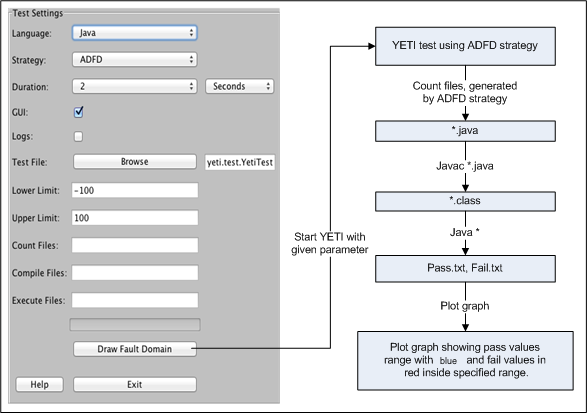
\includegraphics[width=15cm,height=11cm]{chapter5/ADFD_Diagram1.png}
\bigskip
\caption{Work-flow of ADFD strategy}
\label{fig:ADFD-workflow}
\end{figure}
\bigskip

\subsection{GUI Front-end for Providing Input}
The ADFD strategy is provided with an easy to use GUI front-end to get input from the user. It takes YETI specific input, including program language, strategy, duration, options to enable or disable YETI GUI, logs and program in byte code. In addition, it also takes minimum and maximum values to search for failure domain in the specified range. Default range for minimum and maximum is taken as Integer.MIN\_VALUE and Integer.MAX\_VALUE respectively. The GUI front-end of ADFD technique is given in Figure~\ref{fig:ADFD-frontend}.


\subsection{Automated Finding of Failure}
ADFD, being extended form of R$^+$ strategy, relies on R$^+$ strategy to find the first failure. Random$^+$ strategy is an improvement on random strategy with preference for the boundary values and other special pre-defined values to provide better failure finding ability. % ADFD strategy is implemented in YETI which is famous for its simplicity, high speed and proven ability of finding potentially hazardous faults in many systems~\cite{Oriol2011, Oriol2012}. YETI is quick and can call up to one million instructions in one second on Java code. It is also capable of testing VB.Net, C, JML and CoFoJa beside Java. \\

\subsection{Automated Generation of Modules}
After a failure is found in the SUT, ADFD strategy generates complete new Java program to search for failure domains in the given SUT.  These programs with ``.java" extensions are generated through dynamic compiler API included in Java 6 under javax.tools package. The number of programs generated can be one or more, depending on the number of arguments in the test module i.e. for module with one argument one program is generated, for module with two arguments two programs and so on. To track failure domain, the program keeps only one argument as variable and the remaining arguments as constant in the program generated at run time.

\begin{figure}[H]
\begin{center}
%\centring
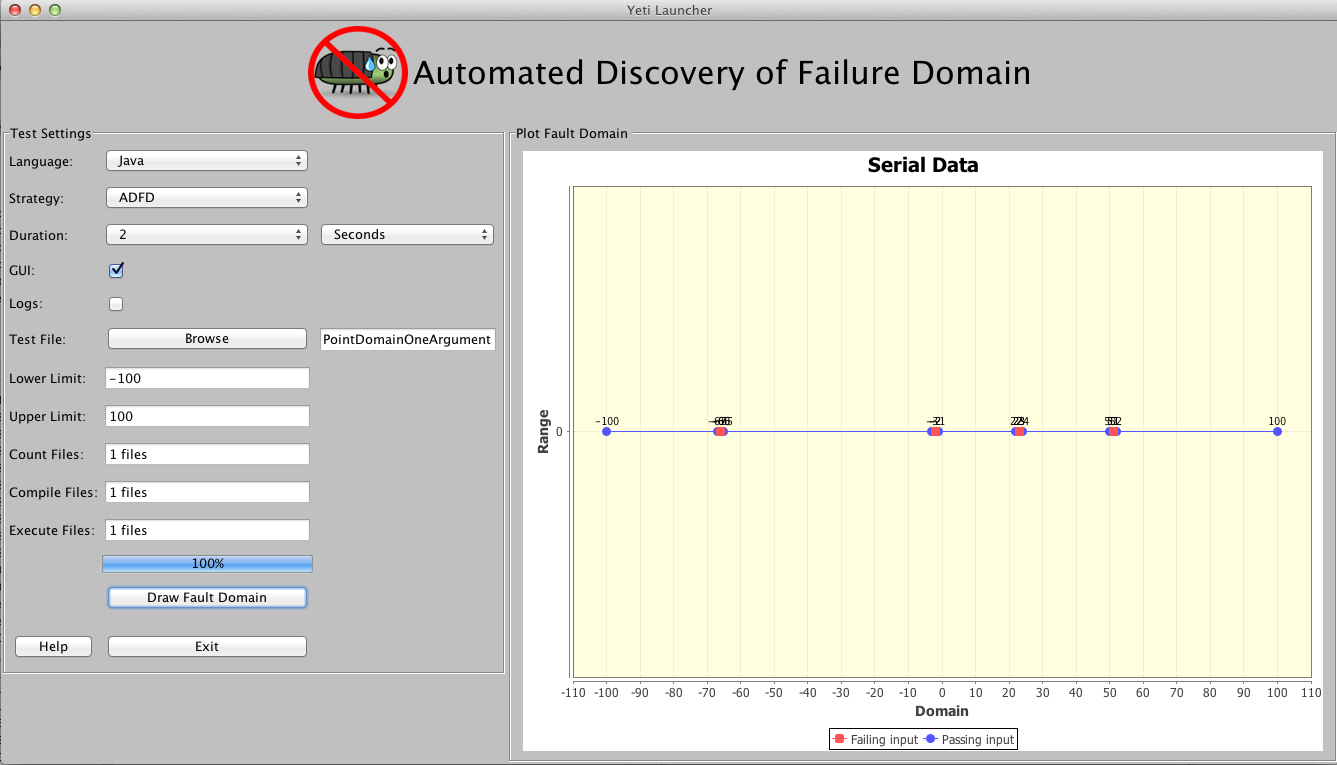
\includegraphics[width=15cm,height=11cm]{chapter5/ADFD_front_end.png}
\bigskip
\caption{Front-end of ADFD strategy}
\label{fig:ADFD-frontend}
\end{center}
\end{figure}
\bigskip

\subsection{Automated Compilation and Execution of Modules}
The java modules generated in the previous step are compiled using $javac~*$ command to get their binary $.class$ files. The $java~*$ command is applied to execute the compiled programs. During execution, the constant arguments of the module remain the same but the variable argument receives all the values ranging, from minimum to maximum, specified at the beginning of the test. After execution is completed we get two text files of $Pass.txt$ and $Fail.txt$. Pass file contains all the values for which the modules behave correctly while fail file contains all the values for which the modules fail.

\subsection{Automated Generation of Graph}
The values from the pass and fail files are used to plot (x, y) chart using JFreeChart~\cite{gilbert2008jfreechart}. JFreeChart is a free open-source Java library that helps developers to display complex charts and graphs. Among several types of available chart, Line chart is selected because it can represent the available data in the most effective way. The Lines and circles with blue colour represent pass values while lines and squares with red colour represents fail values. Resultant graph clearly depicts both the pass and fail domain across the specified input domain. The graph shows red points when the program fails for only one value, blocks when the program fails for multiple values and strips when the program fails for a long range of values.%\subsection{Flow Chart of the process}

%The following flow chart clearly identify the workflow of the whole process and the various steps involved in the process.

%\begin{figure}[p]
%\centering
%\includegraphics[width=8cm,height=12cm]{automatedFail.png}
%\caption{Automated discovery of Failure Domain}
%\label{fig:autofail}
%\end{figure}




%We found that it is better for the developer to see the range because the fault can be found once but it can generate errors at multiple locations.like point pattern in the first graph only generate fault at location 0 but if the same zero is assigned to second argument then the whole domain values can fail.\\


%\begin{figure}[htp]
%\centering
%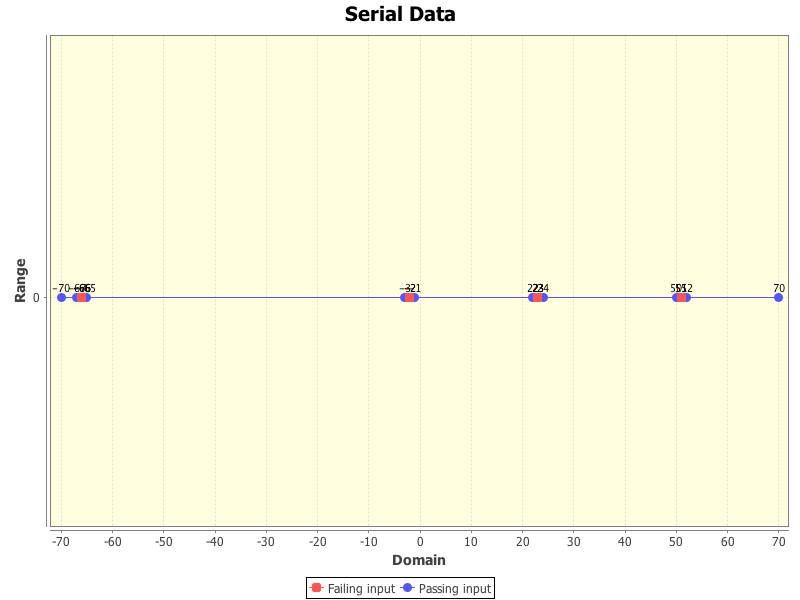
\includegraphics[width=8.5cm,height=6cm]{oneArgumentPointDomain.png}
%\caption{Point pattern failure domain}
%\label{fig:patterns}
%\end{figure}


%Figure \ref{fig:point} shows the example of point pattern. In sub figure \ref{fig1:a} test only fails for 0 out of the whole integer range where as in sub figure \ref{fig1:b} all test fails when static variable is assigned with 0 value.


%\begin{figure}[htp]
%\centering
%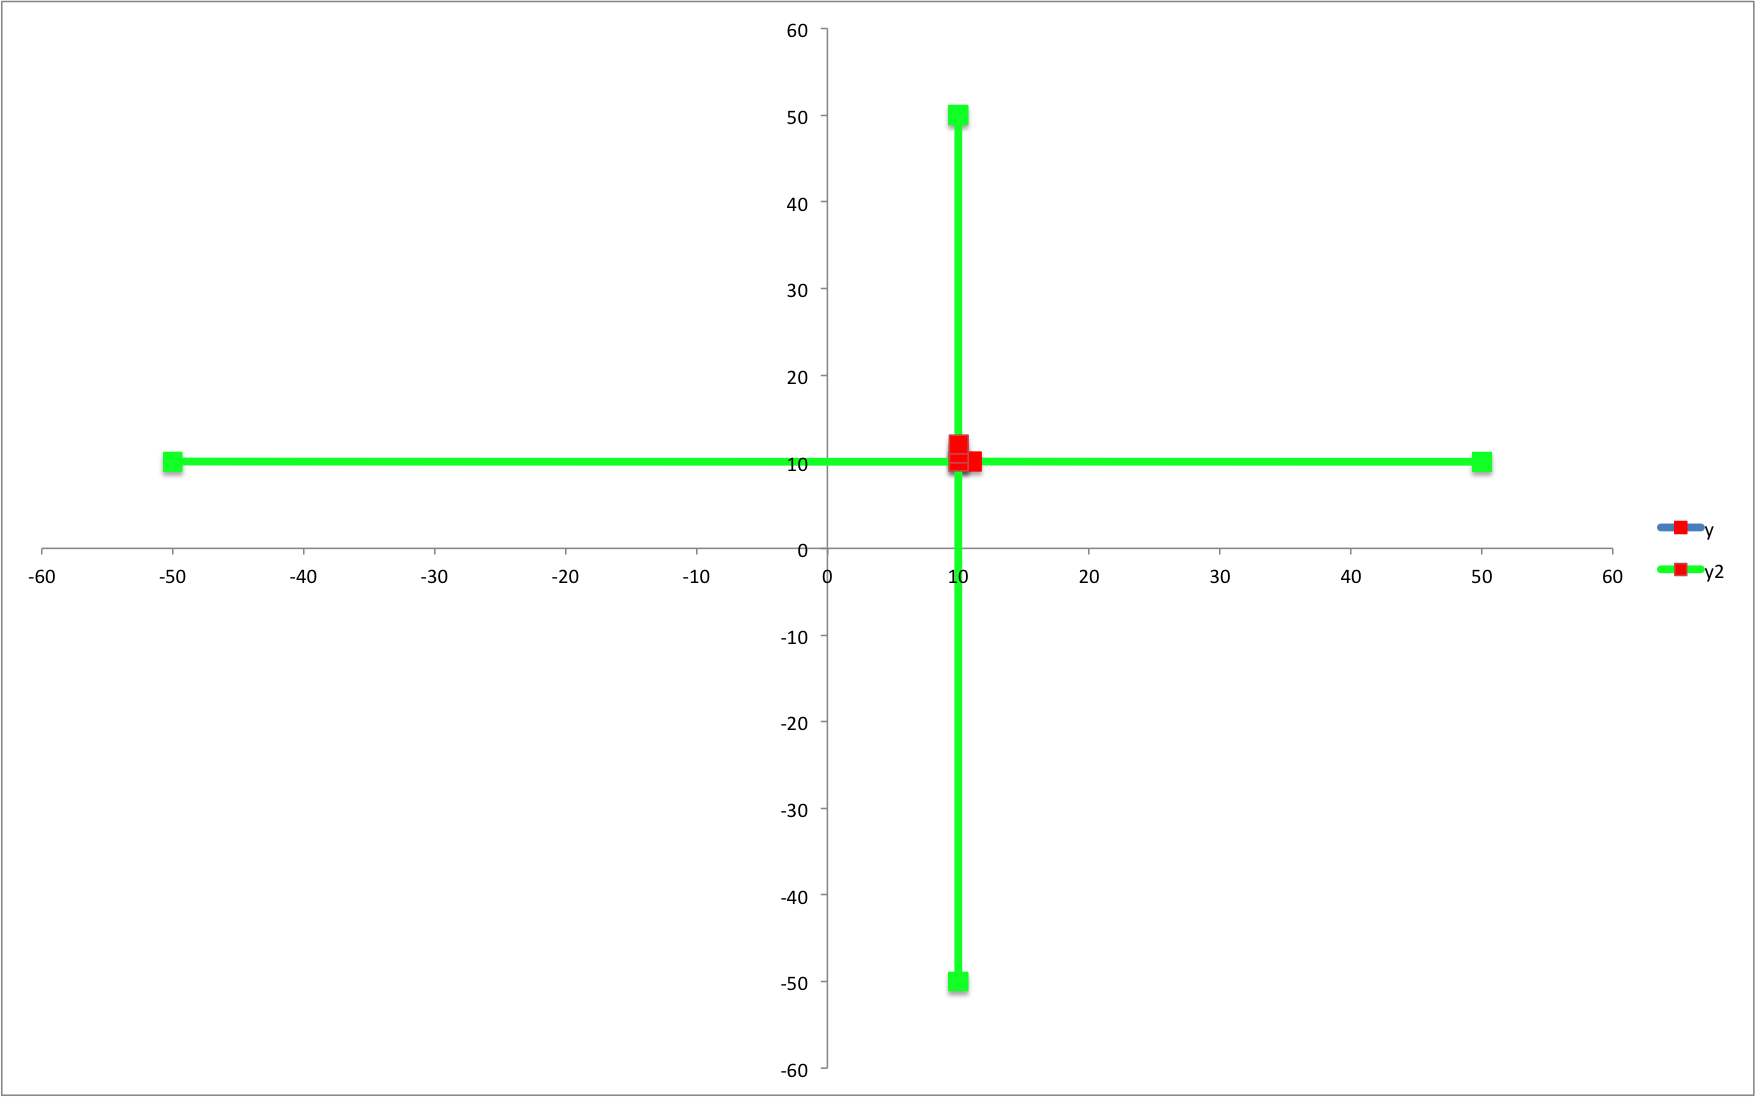
\includegraphics[width=4cm,height=4cm]{block_pattern.png}
%\caption{Block pattern failure domain}
%\label{fig:patterns}
%\end{figure}


%Figure \ref{fig:block} shows the example of block pattern. Both sub figure \ref{fig1:a} and \ref{fig1:b} shows the block pattern of failure. The failure values are given in table \ref{tb:failtable}.

%\begin{figure}[htp]
%\centering
%\begin{center}
%  % Maximum length
 %\subfloat[Test 1 A]{\label{fig1:a}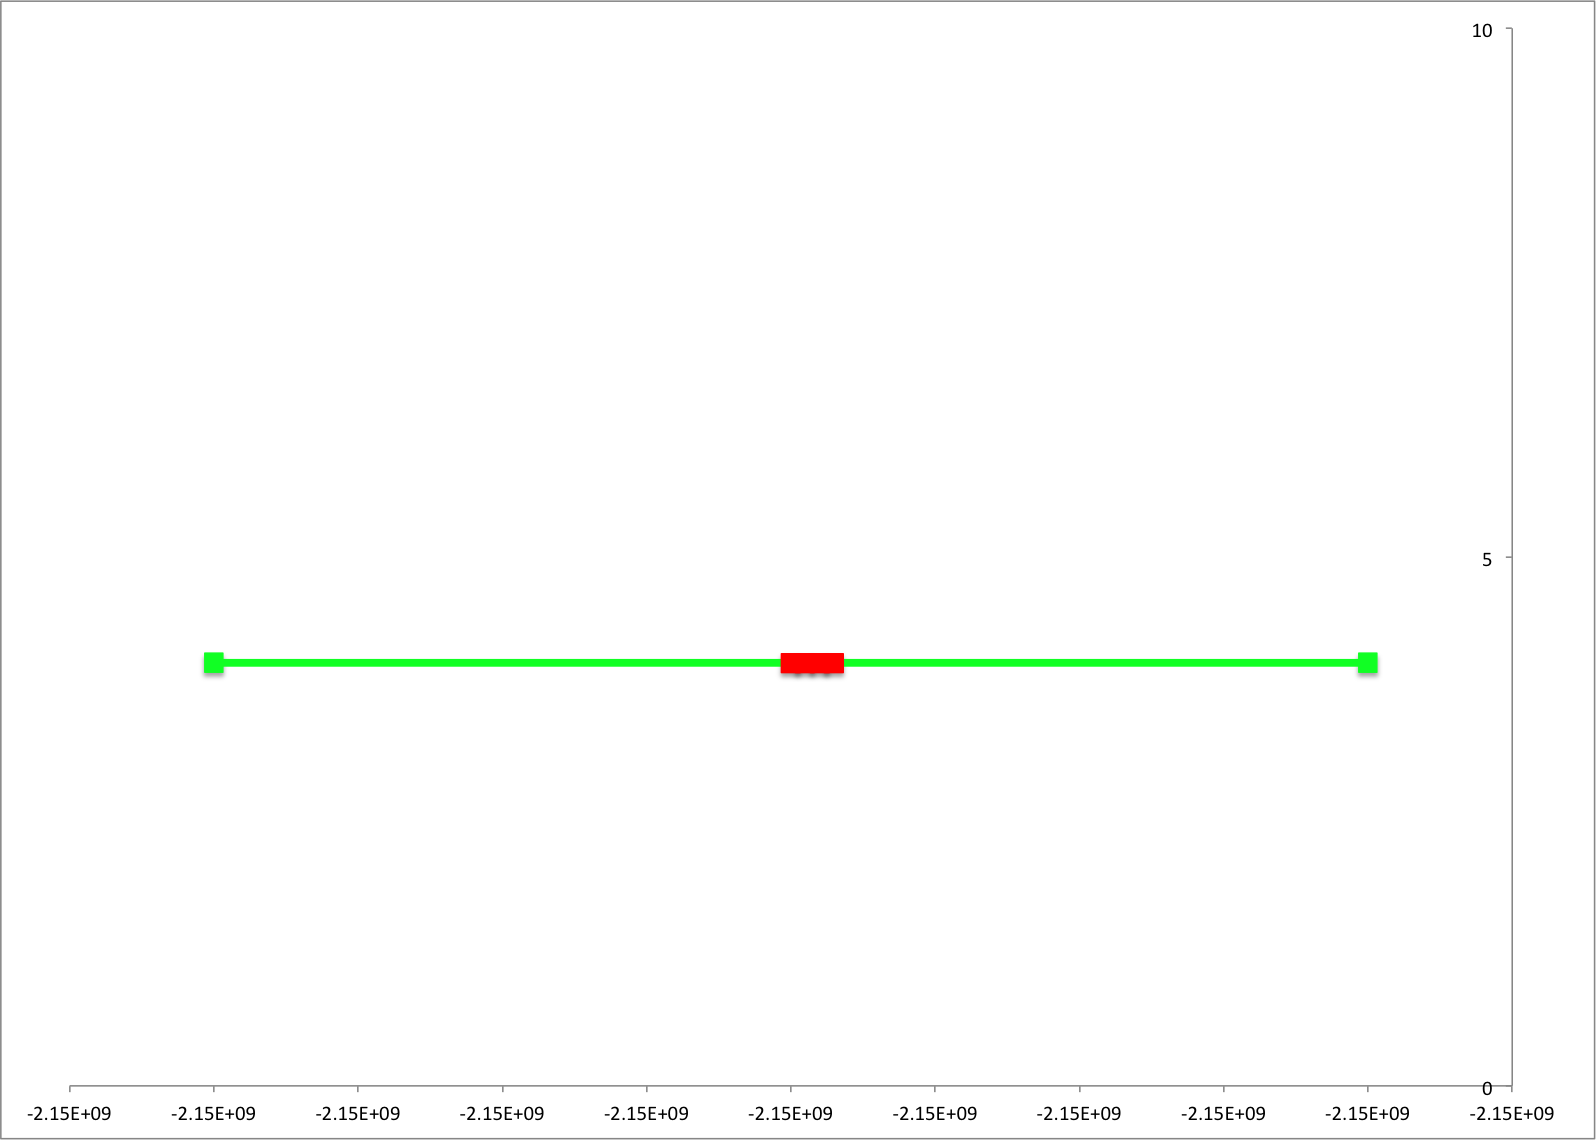
\includegraphics[width=0.49\linewidth]{excel_png/strip_pattern_B.png}}\hfill
 %\subfloat[Test 1 B]{\label{fig1:b}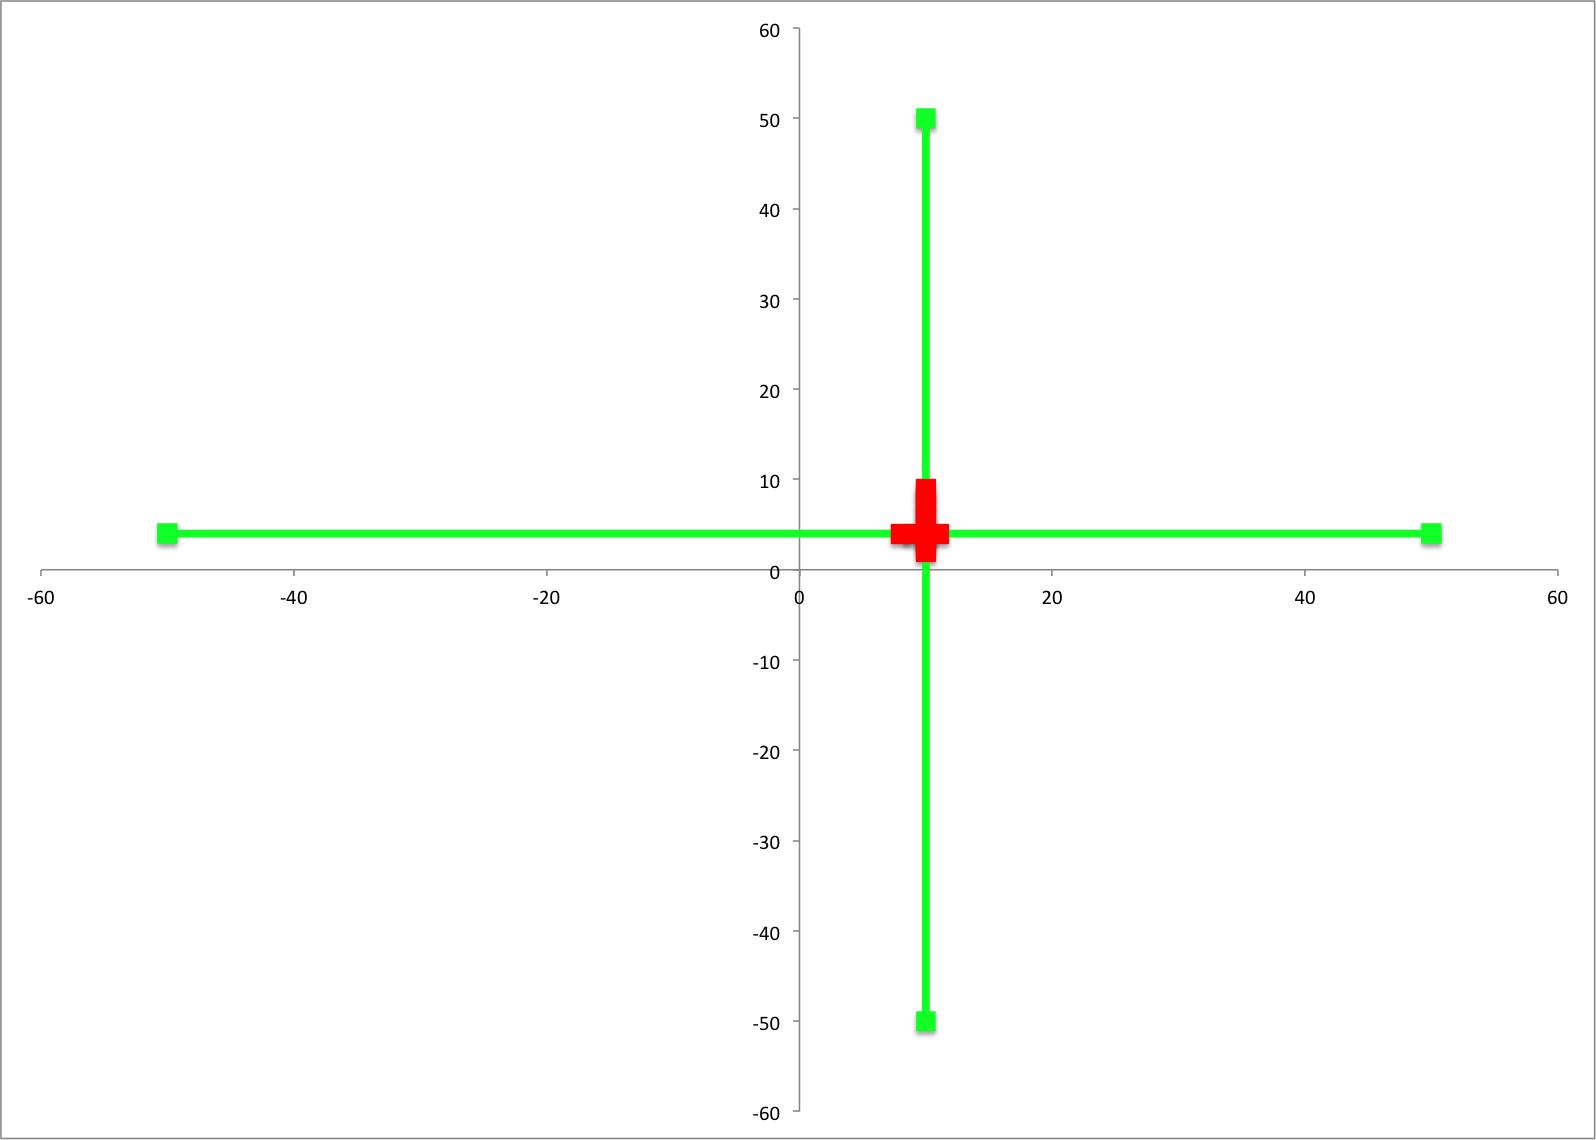
\includegraphics[width=0.49\linewidth]{excel_png/strip_pattern_A.png}}
%  end{center}
%\caption{Strip pattern failure domain}
%%  \label{fig:strip}
%\end{figure}

%Figure shows the example of strip pattern. Here we have two strip failure pattern for test 1 shown in \ref{fig1:a} and \ref{fig1:b} while 1 other for test 2 given in . The failure values are given in table .\\

\subsection{Implementation of ADFD Strategy}\label{sec:implementation}
The ADFD strategy is implemented as a strategy of YETI (see Chapter~\ref{chap:yeti_3} for more details on YETI). This section contains various strategies including random, random$^+$ and DSSR to be selected for testing according to the specific needs. The default strategy for testing YETI is random. On top of the hierarchy in strategies section, is an abstract class YetiStrategy, which is extended by YetiRandomStrategy and it is further extended to get YetiRandomPlusStrategy. YetiADFDStrategy is developed by extending the YetiRandomPlusStrategy.

% The ADFD strategy is also implemented in YETI (see Chapter~\ref{chap:yeti_3} for details on YETI).  In this section, we give a brief overview of the implementation of ADFD strategy in YETI and illustrate it with the help of an example. 

\begin{figure}[h]
\centering
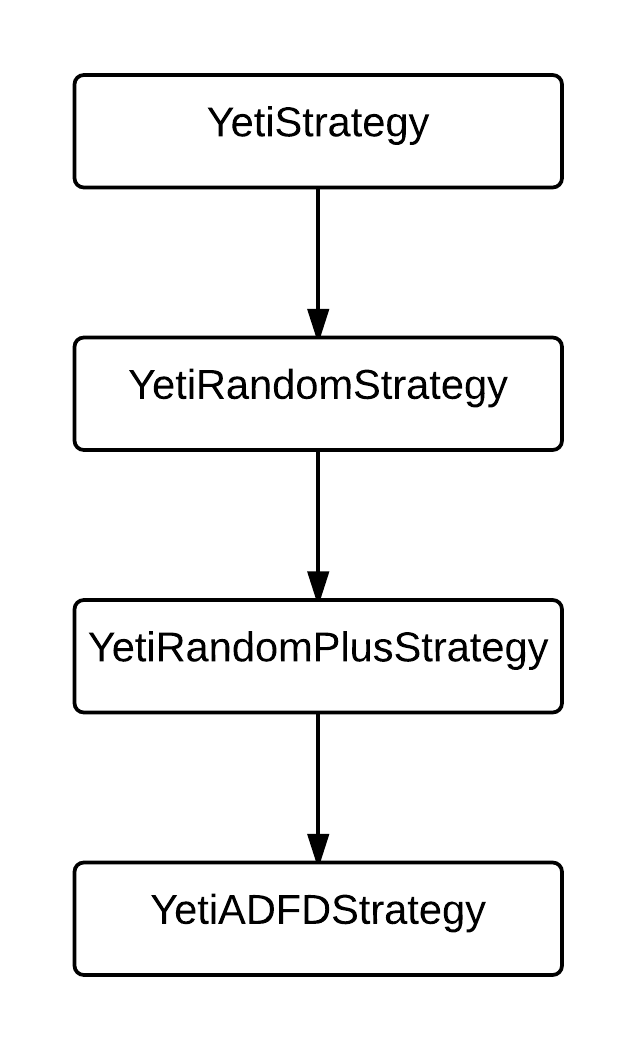
\includegraphics[width=6cm,height=9.5cm]{chapter5/classHierarchy2.png}
\bigskip
\caption{Class Hierarchy of ADFD strategy in YETI}
\label{fig:hierarchyofADFD}
\end{figure}

%\subsection{York Extensible Testing Infrastructure}
%YETI is a testing tool developed in Java that tests programs using random strategies in an automated fashion. YETI meta-model is language-agnostic which enables it to test programs written in functional, procedural and object-oriented languages.

%YETI consists of three main parts including core infrastructure for extendibility through specialisation, strategies section for adjustment of multiple strategies and languages section for supporting multiple languages. Both the languages and strategies sections have a pluggable architecture to easily incorporate new strategies and languages making YETI a favourable choice to implement ADFD strategy. YETI is also capable of generating test cases to reproduce the failures found during the test session.
 
% \subsection{ADFD strategy in YETI}
%ADFD strategy is implemented in the strategies section of YETI. This section contains various strategies including random, random$^+$ and DSSR to be selected for testing according to the specific needs. The default strategy for testing YETI is random. On top of the hierarchy in strategies section, is an abstract class YetiStrategy, which is extended by YetiRandomStrategy and it is further extended to get YetiRandomPlusStrategy. YetiADFDStrategy is developed by extending the YetiRandomPlusStrategy.



% as shown in figure \ref{fig:hierarchy}. 
 
%\begin{figure}[h]
%\centering
%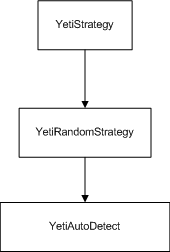
\includegraphics[width=3cm,height=3.5cm]{Hierarchy1.png}
%\caption{Class Hierarchy of automated discovery of failure domains in YETI}
%\label{fig:hierarchy}
%\end{figure}

\subsection{Explanation of ADFD Strategy by Example}\label{sec:example}
For a concrete example to show how ADFD strategy in YETI proceeds, we suppose YETI tests the following class with ADFD strategy selected for testing. Note that for more clear visibility of the output graph generated by ADFD strategy at the end of test session, we set the values of lower and upper range by -70 and 70 from Integer.MIN\_VALUE and Integer.MAX\_VALUE respectively. 

\begin{lstlisting}
/**
 * Point Fault Domain example for one argument program
 * @author (Mian and Manuel)
 */
public class PointDomainOneArgument{
	public static void pointErrors (int x){
 		if (x == -66) 
			 	abort(); 		/* error */
		if (x == -2) 
			 	abort(); 		/* error */
 		if (x == 51) 
			 	abort(); 		/* error */
		if (x == 23) 
			 	abort(); 		/* error */
	}
}
\end{lstlisting}

%Published programs from literature~\cite{Chen2003}\cite{Chan1996}\cite{Chen2004} of point, block and strip failure patterns are tested to explain the working of ADFD . These programs were translated in to java language for this experiment (See appendix 1 for more details). 

\begin{figure}[H]
\centering
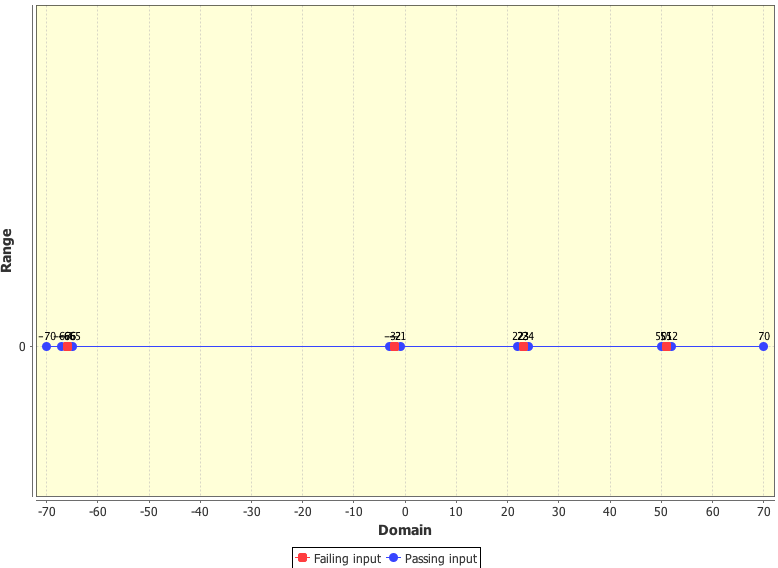
\includegraphics[width=14cm,height=7.5cm]{chapter5/pointDomainOneArgument.png}
\caption{ADFD strategy plotting pass and fail domain of a given class}
\label{fig:ADFD-example}
\end{figure}

As soon as any one of the above four failures are discovered the ADFD strategy generates a dynamic program given in Appendix 1 (7). This program is automatically compiled to get the binary file and then executed to find the pass and fail domains inside the specified range. The identified domains are plotted on a two-dimensional graph. It is evident from the output presented in Figure \ref{fig:ADFD-example} that ADFD strategy not only finds all the failures but also plots the pass and fail domains.


\begin{comment}
%%%%%% They are commented in this format to decrease the text, for two column format uncomment them.

%ADFD can be activated by typing the command java -jar ADFD.jar. After the GUI of ADFD is launched we need to specify yeti specific values that include language of the program under test, strategy for the current test session, duration of test session (minutes or milli-second), display YETI GUI or not and display real time logs or not. Next we browse to select the file for testing and the run button starts testing the file with YETI. 

\bigskip
\begin{figure}[ht]
\centering
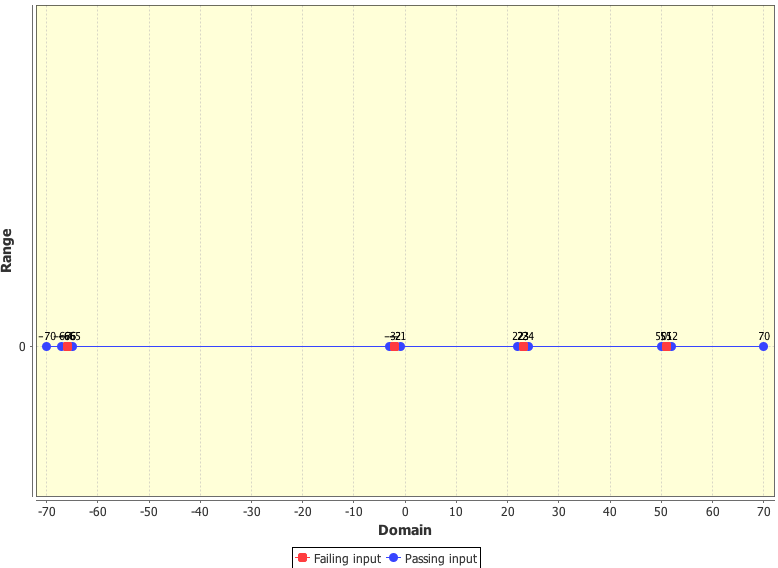
\includegraphics[width=12.2cm,height=8.5cm]{chapter5/pointDomainOneArgument.png}
\bigskip
\caption{ADFD strategy plotting pass and fail domains of the given class}
\label{fig:ADFD-plot}
\end{figure}
\bigskip

%In 5 second YETI found one fault out of the above 4 faults. The ADFD strategy in YETI generate a source file (C*.java) at the end of the test session. This file contain the code that searches for fault domains. The count button count the number of files. ADFD create the number of files on the basis of the number of arguments in the method under test. For one argument one method is created and for two argument two methods are created. 

%The next button is compile which compile the generated files and generate the byte code (.class files). The execute button execute the byte code and test the method under test for all the values between upper and lower bound. At the end of execution it generates two files (pass.txt and fail.txt). Pass file contain all the values for which the method performed correctly while fail file contain all the values for which the method under test fail.

%The draw fault domain button reads the pass and fail files and plot them on the x, y graph where red line with squares show the failing values while the blue line with square shapes show the passing values.
\end{comment}

%%%%%%%%%%%%%%%%%%%%%%%%%%%%%%%%%%%%%%%%%%%%%%%%%%%%%%%%

\section{Experimental Results} \label{sec:experimentalResults}
This section includes the experimental set-up and results obtained by using ADFD strategy. Six numerical programs of one and two-dimension were selected. These programs were error-seeded in such a way to get all the three forms of point, block and strip failure domains. Each selected program contained various combinations of one or more failure domains. 

All experiments were performed on a 64-bit Mac OS X Lion Version 10.7.5 running on 2 x 2.66 GHz 6-Core Intel Xeon with 6.00 GB (1333 MHz DDR3) of RAM. YETI runs on top of the Java\texttrademark  SE Runtime Environment [version 1.6.0\_35]. 

To elucidate the results, six programs were developed so as to have separate program for one and two-dimensional point, block and strip failure domains. The code of the selected program is given in Appendix 1 (1-6). The experimental results are presented in Table \ref{table:failtable} followed by description under three headings.
%To elucidate the results, six programs were developed so as to have separate program for one and two-dimension point, block and strip fault domains. The code of selected programs is given in Appendix \ref{sec:appendix1} (2-7). The experimental results are presented in Table \ref{table:failtable} and described under the following three headings.
%\begin{center}

%\end{center}
\begin{table}[h]
%\renewcommand{\arraystretch}{2}
\caption{Experimental results of programs tested with ADFD strategy}
\bigskip
\centering
{\renewcommand{\arraystretch}{1.3}
\scriptsize
%\normalsize

\begin{tabular}{|c|c|c|l|l|l|}

\hline 


\multirow{2}{*}{S.No}	& \multirow{2}{*}{Fault }	& \multirow{2}{*}{Module} 	& \multirow{2}{*}{Specific Fault}	& \multirow{2}{*}{Pass Domain} 	& \multirow{2}{*}{Fail Domain} \\  
					& Domain				&  Dimension			&								&								&							\\ \hline 
\multirow{6}{*}{1} 	& \multirow{6}{*}{Point}	& \multirow{3}{*}{One}	& \multirow{3}{*}{PFDOneA(i)}		&	-100 to -67, -65 to -3, 		& -66, -2, 23, 51			 	\\  
					&						&						&								&	-1 to 50, 2 to 22, 			&							\\  
					&						&						&								&	24 to 50, 52 to 100			&							\\ \cline{3-6}
					&						& \multirow{3}{*}{Two}	& \multirow{2}{*}{PFDTwoA(2, i)}	&	(2, 100) to (2, 1),	 			&  (2, 0)						\\  
					&						&						&								&	(2, -1) to (2, -100)			&							\\ \cline{4-6}
					&						& 						&	PFDTwoA(i, 0)				&	Nil							& (-100, 0) to (100, 0)		\\  \hline



\multirow{5}{*}{2} 	& \multirow{5}{*}{Block}	& 	\multirow{2}{*}{One}	& \multirow{2}{*}{BFDOneA(i)}		&	-100 to -30, -25 to -2, 		& 	-1 to 1, -29 to -26,		 \\ 
					&						&						&								&	2 to 50, 55 to 100			&	51 to 54,				\\  \cline{3-6}
					&						&	\multirow{3}{*}{Two}	& \multirow{2}{*}{BFDTwoA(-2, i)}	&	(-2, 100) to (-2, 20), 			& 	(-2 , 19) to ( -2, 0), 		\\ 
					&						&						&								&     (-2, -1) to (-2, -100)			&							\\ \cline{4-6}
					&						& 						&	BFDTwoA(i, 0)				&	Nil							& 	(-100, 0) to (100, 0)		\\  \hline
				
				



\multirow{5}{*}{3} 	& \multirow{5}{*}{Strip}	& 	\multirow{2}{*}{One}	&	\multirow{2}{*}{SFDOneA(i)}	& \multirow{2}{*}{-100 to -5, 35 to 100}& 	\multirow{2}{*}{-4 to 34}	\\ 
					&						&						&								&									 &						\\ \cline{3-6}
					&						&	\multirow{3}{*}{Two}	& \multirow{2}{*}{SFDTwoA(-5, i)}	&	(-5, 100) to (-5, 40),				 &  (-5, 39) to (-5, 0), 		\\ 
					&						&						&								&	 (-5, -1) to (-5, -100)				&						\\ \cline{4-6}
					&						& 						&	SFDTwoA(i, 0)				&	Nil								&  (-100, 0) to (100, 0)	\\  \hline
				
				
\end{tabular}
}
\label{table:failtable}
\end{table}

\bigskip

\textbf{Point Failure Domain:}  Two separate Java programs \verb+Program1+ and \verb+Program2+, given in Appendix 1 (1, 2), were tested with ADFD strategy in YETI to get the findings for point failure domain in one and two-dimension program. Figure \ref{fig:PFDOne} presents range of pass and fail values for point failure domain in one-dimension whereas Figure \ref{fig:PFDTwo} presents range of pass and fail values for point failure domain in two-dimension program. The range of pass and fail values for each program in point failure domain is given in Table \ref{table:failtable}.
%%%%%%%%%%%%%%%%Point Domain%%%%%%%%%%%%%%%%%%%%%%%%%%%%%

\begin{figure} [H]
\centering
\subfigure[One dimension module]{
\includegraphics[width=15cm,height=7.5cm]{chapter5/PFDOne.png}
\label{fig:PFDOne}
}

\bigskip
\subfigure[Two dimension module]{
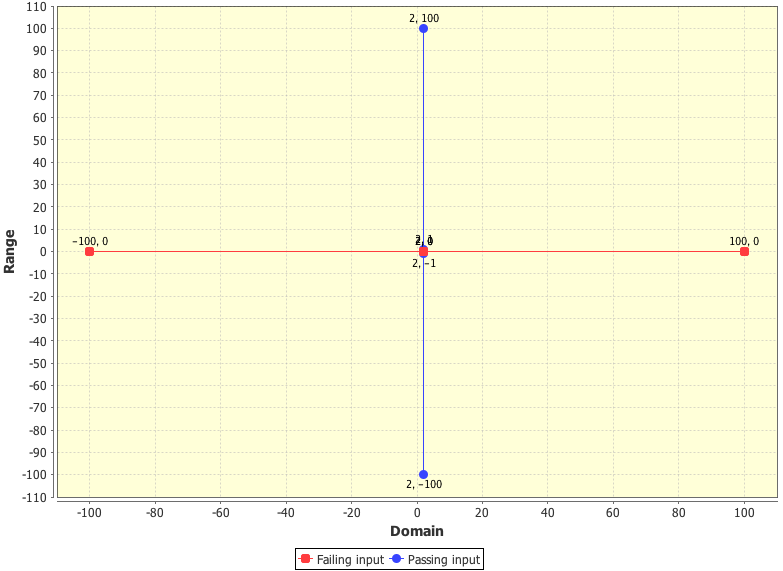
\includegraphics[width=15cm,height=7.5cm]{chapter5/PFDTwo.png}
\label{fig:PFDTwo}
}
\bigskip
\caption{Chart generated by ADFD strategy presenting point failure domain}
\end{figure}
\bigskip
%\begin{figure}[H]
%\centering
%\includegraphics[width=8.2cm,height=5cm]{PFDOne.png}
%\caption{Chart generated by ADFD strategy presenting point fault domain in one dimension module}
%\label{fig:PFDOne}
%\end{figure}

%\begin{figure}[H]
%\centering
%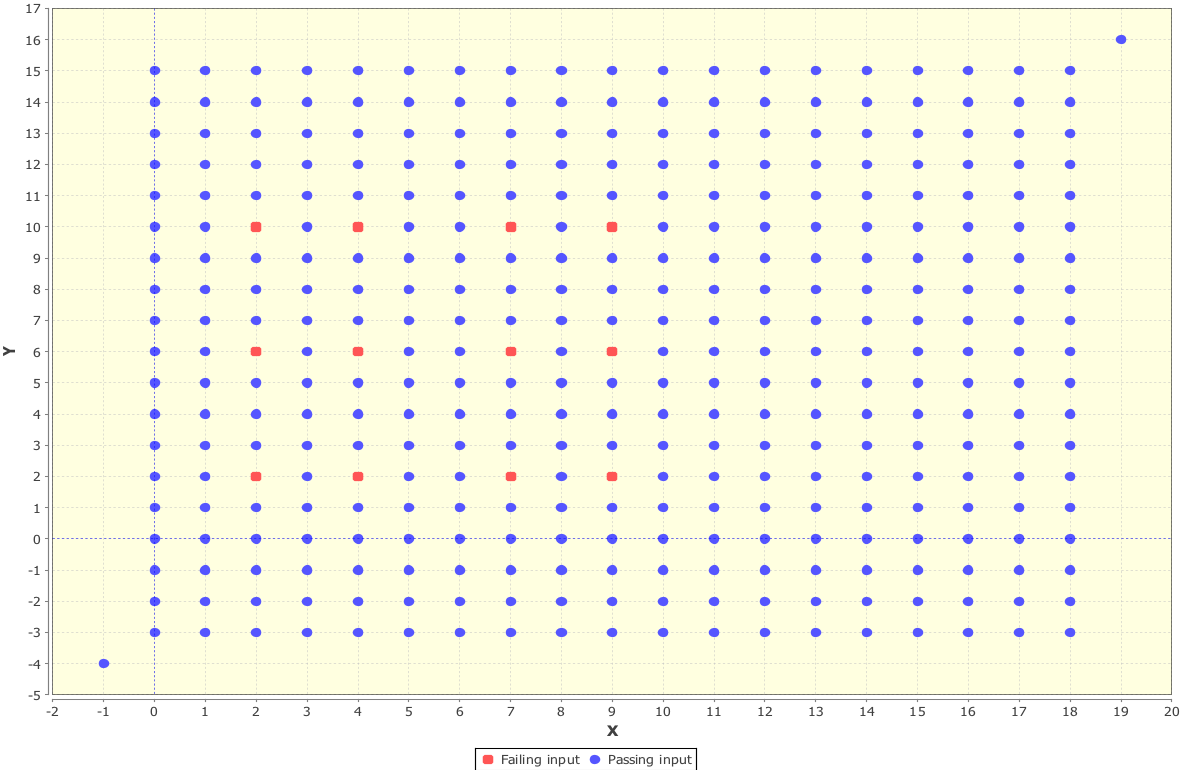
\includegraphics[width=8.2cm,height=5cm]{PFDTwo.png}
%\caption{Chart generated by ADFD strategy presenting point fault domain in two dimension module}
%\label{fig:PFDTwo}
%\end{figure}

\newpage
\noindent \textbf{Block Failure Domain:}  Two separate Java programs \verb+Program3+ and \verb+Program4+ given in Appendix 1 (3, 4) were tested with ADFD strategy in YETI to get the findings for block failure domain in one and two-dimension program. Figure \ref{fig:BFDOne} presents a range of pass and fail values for block failure domain in one-dimension whereas Figure \ref{fig:BFDTwo} presents a range of pass and fail values for block failure domain in two-dimension program. The range of pass and fail values for each program in block failure domain is given in Table \ref{table:failtable}.
%%%%%%%%%%%%%%%Block domain %%%%%%%%%%%%%%%%%%%%%%%%%%%%%%
%%%





\begin{figure} [H]
\centering
\subfigure[One dimension module]{
\includegraphics[width=15cm,height=7.5cm]{chapter5/BFDOne.png}
\label{fig:BFDOne}
}
\bigskip

\subfigure[Two dimension module]{
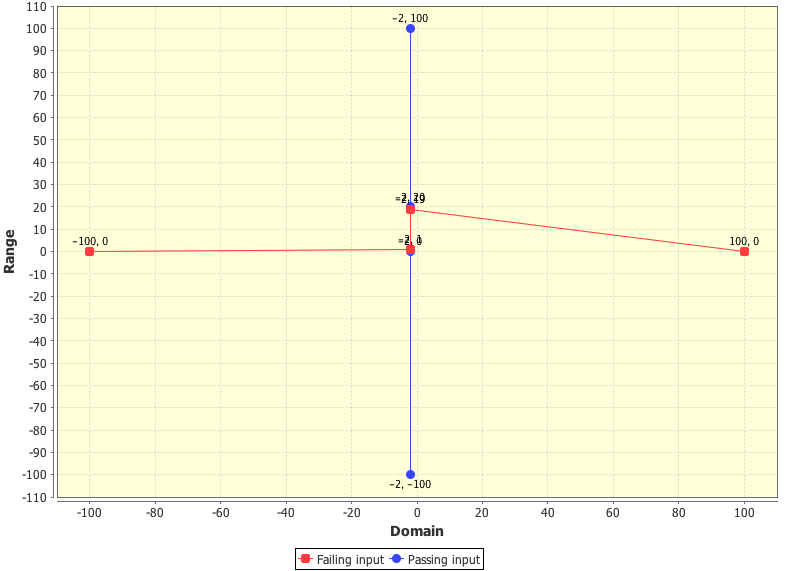
\includegraphics[width=15cm,height=7.5cm]{chapter5/BFDTwo.png}
\label{fig:BFDTwo}
}
\bigskip
\caption{Chart generated by ADFD strategy presenting block failure domain}
\end{figure}


%\begin{figure}[H]
%\centering
%\includegraphics[width=8.2cm,height=5cm]{BFDOne.png}
%\caption{Chart generated by ADFD strategy presenting block fault domain in one dimension module}
%\label{fig:BFDOne}
%\end{figure}


%\begin{figure}[H]
%\centering
%\includegraphics[width=8.2cm,height=5cm]{BFDTwo.png}
%\caption{Chart generated by ADFD strategy presenting block fault domain in two dimension module}
%\label{fig:BFDTwo}
%\end{figure}


\newpage
\noindent \textbf{Strip Failure Domain:} Two separate Java programs \verb+Program5+ and \verb+Program6+ given in Appendix 1 (5, 6) were tested with ADFD strategy in YETI to get the findings for strip failure domain in one and two-dimension program. Figure \ref{fig:SFDOne} presents range of pass and fail values for strip failure domain in one-dimension whereas Figure \ref{fig:SFDTwo} presents a range of pass and fail values for strip failure domain in two-dimension program. The range of pass and fail values for each program in strip failure domain is given in Table \ref{table:failtable}.


%
%%%%%%%%%%%%%%%%%%%%%%Strip domain %%%%%%%%%%%%%%%%%%%%%%%
\begin{figure} [H]
\centering
\subfigure[One dimension module]{
\includegraphics[width=15cm,height=7.5cm]{chapter5/SFDOne.png}
\label{fig:SFDOne}
}
\bigskip
\subfigure[Two dimension module]{
\includegraphics[width=15cm,height=7.5cm]{chapter5/SFDTwo.png}
\label{fig:SFDTwo}
}
\bigskip
\caption{Chart generated by ADFD strategy presenting Strip failure domain}
\end{figure}






%\begin{figure}[H]
%\centering
%\includegraphics[width=8.2cm,height=5cm]{SFDOne.png}
%\caption{Chart generated by ADFD strategy presenting strip fault domain in one dimension module}
%\label{fig:SFDOne}
%\end{figure}

%\begin{figure}[H]
%\centering
%\includegraphics[width=8.2cm,height=5cm]{SFDTwo.png}
%\caption{Chart generated by ADFD strategy presenting strip fault domain in two dimension module}
%\label{fig:SFDTwo}
%\end{figure}



\section{Discussion} \label{sec:discussion4}

The ADFD, with a simple graphical user interface, is a fully automated testing strategy which identifies failures, failure domains and visually present the pass and fail domains in the form of a chart. Since all the default settings are set to the optimum level, the user needs only to specify the module to be tested and click ``Draw fault domain" button to start test execution. All the steps including Identification of fault, generation of dynamic Java program to find domain of the identified failure, saving the program to a permanent media, compiling the program to get its binary, execution of binaries to get pass and fail domain and plotting these values on the graph are done completely automatically without any human intervention.

As evident from the results, ADFD strategy effectively identified failures and failure domains in selected programs. Identification of the failure domain is simple for one and two-dimensional numerical program but as the dimension increases the process gets more and more complicated. Moreover, no clear boundaries are defined for non-numerical data, therefore, it is not possible to plot domains for non-numerical data unless some boundary criteria are defined.

ADFD strategy initiates testing with R$^+$ strategy to find the failure and later switches to exhaustive strategy to apply all the values between upper and lower bounds for finding pass and failure domains. It was found that failures at boundary of the input domain usually passes unnoticed through random test strategy~\cite{reid1997empirical} but not through ADFD strategy because it scans all the values between lower and upper bounds.


The overhead in terms of execution time associated with ADFD strategy is dependent mainly on the lower and upper bounds. If the lower and upper bounds are set to the maximum range (i.e. minimum for int is Integer.MIN\_VALUE and maximum Integer.MAX\_VALUE) then the test duration is also maximum. It is rightly so because for identification of the failure domain the program is executed for every input available in the specified range. Similarly increasing the range also shrinks the produced graph making it difficult to identify clearly point, block and strip domains unless they are of considerable size. Test duration is also influenced by identification of the first failure and the complexity of the module under test.

ADFD strategy can help the developers in two ways. First, it reduces the `to' and `from' movement of the program between the testers and debuggers as it identifies all the failures in one go. Second, it identifies locations of all failure domains across the input domain in a user-friendly way helping debugger to fix the fault keeping in view its all occurrences.


\section{Threats to Validity} \label{sec:validity}
The major external threat to the use of ADFD strategy on a commercial scale is the selection of a small set of error-seeded programs of only primitive types such as integer used in the experiments. However, the present study will serve as the foundation for future work to expand it to general-purpose real world production application containing scalar and non-scalar data types.

Another issue is the plotting of the objects in the form of distinctive units, because it is difficult to split the composite objects containing many fields into units for plotting. Some work has been done to quantify composite objects into units on the basis of multiple features~\cite{ciupa2006object}, to facilitate easy plotting. Plotting composite objects is beyond the scope of the present study. However, further studies are required to look into the matter in depth. 

Another threat to validity includes evaluating program with complex and more than two input arguments. In the current study, ADFD strategy has only considered scalar data of one and two-dimensions. Plotting domain of programs with complex non-scalar and more than two dimension argument is much more complicated and needs to be taken up in future studies.

Finally, plotting the range of pass or fail values for a large input domain (Integer.MIN\_VALUE to Integer.MAX\_VALUE) is difficult to adjust and does not give a clear view on the chart. To solve this problem, zoom feature was incorporated into the strategy to magnify the areas of interest on the chart.



\section{Related Work} \label{sec:relatedWork}
Traditional random testing is quick, easy to implement and free from any bias. In spite of these benefits, the lower fault finding ability of traditional random testing is often criticised~\cite{myers2011art, offutt1996semantic}. To overcome the performance issues without compromising on its benefits, various researchers have altered its algorithm as explained in Section~\ref{sec:versionsOfRT}. Most of the alterations are based on the existence of faults and failure domains across the input domain~\cite{chan1996proportional}. 

Identification, classification of pass and fail domains and visualisation of domains have not received due attention of the researchers. Podgurski et al.~\cite{podgurski2003automated} proposed a semi-automated procedure to classify faults and plot them by using a Hierarchical Multi Dimension Scaling (HMDS) algorithm. A tool named Xslice~\cite{agrawal1995fault} visually differentiates the execution slices of passing and failing part of the test. Another tool called Tarantula uses colour coding to track the statements of a program during and after the execution of the test suite~\cite{jones2002visualization}. A serious limitation of the above-mentioned tools is that they are not fully automated and require human intervention during execution. Moreover, these tools are based on the availability of existing test cases whereas ADFD strategy generates new test cases, discovers faults, identifies pass and fail domains and visualises them in graphical form in a fully automated manner. 


\section{Summary} \label{sec:conclusion}
The newly developed ADFD technique identifies failure, failure domains and graphically represent the test results using XY line chart. Experimental results obtained by applying ADFD strategy to error-seeded numerical programs provide evidence that the strategy is highly effective in identifying the failures and plotting pass and fail domains of a given SUT. ADFD strategy can find boundary failures quickly as against the traditional random testing, which is either, unable or takes comparatively longer time to discover the failures.

The use of ADFD strategy is highly effective in testing and debugging. It provides an easy to understand test report visualising pass and fail domains. It reduces the number of switches of SUT between testers and debuggers because all the faults are identified with a single execution. It improves debugging efficiency as the debuggers keep all the instances of a fault under consideration during debugging. The strategy has the potential to be used at large scale. However, future studies are required to use it with programs of more than two-dimension and different non-scaler argument types.






% ------------------------------------------------------------------------


%%% Local Variables: 
%%% mode: latex
%%% TeX-master: "../thesis"
%%% End: 

\externaldocument{chapter6}
\chapter{Automated Discovery of Failure Domain Plus}
\label{chap:ADFD+}

%This paper presents Automated Discovery of Failure Domain+ (ADFD+), an upgraded version of ADFD technique with respect to algorithm and graphical presentation of failure domains. The new algorithm used in ADFD+ searches for failure domain around the failure in a given radius as against ADFD which limits the search between lower and upper bounds. This results in consumption of lower number of test cases for detecting failure domain. The output has been improved in ADFD+ to provide labelled graphs for depicting the results in easily understandable user friendly form. ADFD+ is compared with Randoop to find the comparative performance of the two techniques. The results indicate that ADFD+ is a promising technique for finding failure and failure domain efficiently and effectively. In comparison with Randoop, its efficiency is evident by taking two orders of magnitude less time and its effectiveness is shown by taking 50\% or less number of test cases to discover failure domains. ADFD+ has the added advantage of presenting the output in graphical form showing point, block and strip domains visually as against Randoop which lacks graphical user interface.




%This paper presents Automated Discovery of Failure Domain+ (ADFD+), an improvement on our previously developed Automated Discovery of Failure Domain (ADFD) technique.  ADFD+ is a random testing technique which after identifying a failure searches its surrounding to find its domain within the set range. The result obtained is graphically presented. To find the effectiveness of our Technique, several error-seeded one and two-dimensional numerical programs fwith point, block and strip failure domain were evaluated independently for 30 times by both ADFD+ and Randoop. Results indicated that ADFD+ can identify failure and failure-domain sufficiently quick and in fewer number of test cases as compared to Randoop. Additionally ADFD+ presents the failure and failure domains in a graphical form.
%\end{abstract}

%A category including the fourth, optional field follows...
%\category{D.2.5}{Software Engineering}{Metrics}[complexity measures, performance measures]

%\terms{Comparison, Verification, }
%\terms{software testing, automated random testing, ADFD}
%\begin{IEEEkeywords}
%software testing, automated random testing, ADFD.
%\end{IEEEkeywords}}


%\IEEEpeerreviewmaketitle



%%%%%%%%%%%%%%%%%    INTRODUCTION   %%%%%%%%%%%%%%%%%%%%

\section{Introduction}\label{sec:intro6}
Software testing is most widely used for verification and validation process. Efforts have been continuously made by researchers to make the testing process more and more effective and efficient. Testing is efficient when maximum number of test cases are executed in minimum possible time and it is effective when it finds the maximum number of faults in minimum number of test cases~\cite{runeson2006we}. During up-gradation and development of testing techniques, focus is always on increasing the efficiency by introducing partial or complete automation of the testing process and the effectiveness by improving the algorithm. 

%\blfootnote{Manuscript received Feb 5, 2014; revised March 20, 2013. The authors are with the Department of Computer Science, University of York, YO10 5DD, UK (e-mail: mian.ahmad@york.ac.uk, manuel.oriol@york.ac.uk).}

%Boundary Value Analysis (BVA) is one of the technique used of increasing test effectiveness. In BVA test cases with boundary values are added to the test suite with the assumption that errors reside along the boundaries~\cite{radatz1990ieee}. Daikon~\cite{ernst2007daikon} is an automatic tool used to improve the efficiency. It saves testers time by automatically generating likely program invariants.
%However, the two approaches can adversely affect the testing process if wrong boundaries or invariants are taken into consideration. It is therefore motivating to accurately identify the boundaries of the input domain in BVA and measure the degree of correctness of auto-generated invariants by Daikon in the case of point, block and strip failure domain. 


%A number of empirical evidence confirms that failure revealing test cases tend to cluster in contiguous regions across the input domain~\cite{finelli1991nasa, schneckenburger2007towards}. According to Chan et al.~\cite{chan1996proportional} the clusters are arranged in the form of point, block and strip failure domains. In the point domain the failure revealing inputs stand-alone and are evenly spread throughout the input domain. In block domain, the failure revealing inputs are contiguously clustered in one area. In strip domain, the failure revealing inputs are clustered in one long elongated strip.  %Figure~\ref{fig:patterns2} shows failure domains of the three types for two-dimensional program. 


To target failures and evaluate the failure domains we developed earlier ADFD technique \cite{ahmad2013adfd}. The ADFD$^+$, an improved version of ADFD, is a fully automatic technique which finds failures and failure domains within a specified radius and presents the results on a graphical chart. The efficiency and effectiveness of ADFD$^+$ technique is evaluated by comparing its performance with that of a mature testing tool Random tester for object-oriented programs (Randoop)~\cite{pacheco2007randoop}. The results generated by ADFD$^+$ and Randoop for the error-seeded programs shows better performance of ADFD$^+$ with respect to time and number of test cases to find failure domains. Additionally ADFD$^+$ presents the results graphically showing identified point block and strip domains visually as against Randoop, which lacks graphical user interface.
%\begin{figure}[H]                                    
%\centering
%\includegraphics[width= 7cm,height=2cm]{ART_Patterns.png}
%\caption{Failure domains across input domain~\cite{chan1996proportional}}
%\label{fig:failurePatterns}
%\end{figure}
%\begin{figure} [H]
%\centering
%\subfigure[Point domain]{
%\includegraphics[width=2.5cm,height=2cm]{point.png}
%\label{fig:point}
%}
%\subfigure[Block domain]{
%\includegraphics[width=2.5cm,height=2cm]{block.png}
%\label{fig:block}
%}
%\subfigure[Strip domain]{
%\includegraphics[width=2.5cm,height=2cm]{strip.png}
%\label{fig:strip}
%}
%\smallskip
%\caption{Failure domains across input domain~\cite{chan1996proportional}}
%\label{fig:patterns2}
%\end{figure}
%This paper describes the new ADFD+ technique developed for automatically finding failures, failure domains and graphical presentation of results. In this technique, the test execution is initiated by random+  and continues till the first failure is found in the SUT. The technique then copies the values leading to the failure and the surrounding values to the dynamic list of interesting values. The resultant list provides relevant test data for the remaining test session and the generated test cases are more targeted towards finding new failures around the existing failures in the given SUT.
%The technique uses random+ \cite{Ciupa2007, ciupa2008finding} in the initial phase. After identification of a failure, ADFD+ searches its surrounding to find its failure domain within the specified range. 


%The rest of the paper is organized as follows: Section II presents an overview of ADFD+ technique. Section III evaluates and compares ADFD+ technique with Randoop. Section IV reveals results of the experiments. Section V discusses the results. Section VI presents the threats to validity. Section VII presents related work. Finally, Section VIII concludes the study.

%The main contributions of the study are:
%\begin{itemize}
%\item \textbf{ADFD+:} It is an extension of Automated Discovery of Failure Domain (ADFD) strategy developed by Ahmad and Oriol~\cite{ahmad2013adfd}. The new technique improves the search algorithm of ADFD and makes the report more intuitive (Section \ref{sec:adfd+}).
%\item \textbf{Implementation of ADFD+:} It is implemented and intgrated in the York Extensible Testing Infrastructure \cite{Oriol2011yeti} (Section \ref{implementation_yeti}).
%\item \textbf{Evaluation:} The results generated by ADFD+ and Randoop about failure domains in the error-seeded programs are evaluated (Section \ref{evaluation}). The results show that although ADFD+ outperform Randoop with respect to time and number of test cases to find a failure domain. Additionally ADFD+ presents the results graphically. 
%\item \textbf{Future work:} ADFD+ can be extended to find and plot failure domains in multi-dimensional non-numerical programs (Section \ref{futurework}).
% A case study suggesting that boundaries are properly recognized by Daikon and ADFD+ or Daikon lake .... etc.
%\end{itemize}
%The rest of this paper is organised as follows: \\ Section~\ref{sec:adfd} describes the ADFD+ strategy. Section~\ref{sec:imp} presents implementation of the ADFD+ strategy. Section~\ref{sec:eval} explains the experimental setup. Section~\ref{sec:res} shows results of the experiments. Section~\ref{sec:discussion} discusses the results. Section~\ref{sec:rw} presents related work and Section~\ref{sec:conc}, concludes the study.


%In the later part we plot the domain on the basis of invariants generated by Daikon and compare both the domains.

%%%%%%%%%%%%%%%%%    Background   %%%%%%%%%%%%%%%%%%%

%\section{Preliminaries} \label{preliminaries}


%In Section~\ref{sec:adfd+} we describe the ADFD+ framework that can find the failure, its domain and plot the domain up to the specified range in a graphical form. Experiments confirms the successful working of ADFD+.


 

%%%%%%%%%%%%%%%%%    ADFD+   %%%%%%%%%%%%%%%%%%%

\section{Automated Discovery of Failure Domain$^+$}\label{sec:adfd+}
It is an improved version of ADFD, a technique developed earlier by Ahmad and Oriol~\cite{ahmad2013adfd}. The technique automatically finds failures, failure domains and present the results in graphical form. In this technique, the test execution is initiated by random$^+$ and continues till the first failure is found in the SUT. The technique then copies the values leading to the failure and the surrounding values to the dynamic list of interesting values. The resultant list provides relevant test data for the remaining test session and the generated test cases are effectively targeted towards finding new failures around the existing failures in the given SUT. \\*
The improvements made in ADFD$^+$ over ADFD technique are stated as follows.
\begin{itemize}
\item ADFD$^+$ generates a single Java file dynamically at run time to plot the failure domains as compared to one Java file per failure in ADFD. This saves sufficient time and makes the execution process quicker.

\item ADFD$^+$ uses (x, y) vector-series to represent failure domains as opposed to the (x, y) line-series in ADFD. The vector-series allows more flexibility and clarity to represent failure and failure domains.   

\item ADFD$^+$ takes a single value for the radius within which the strategy searches for a failure domain whereas ADFD takes two values as lower and upper bounds representing x and y-axis respectively. This results in consumption of the lower number of test cases for detecting failure domain.

\item In ADFD$^+$, the algorithm of dynamically generating Java file at run-time has been made simplified and efficient as compared to ADFD resulting in reduced overhead.

\item In ADFD$^+$, the point, block and strip failure domains generated in the output graph present a clear view of pass and fail domains with individually labelled points of failures as against a less clear view of the pass and fail domains and lack of individually labelled points in ADFD. %The points are also labelled for clarification. % as shown in Figure~\ref{fig:Workflow}. 

%The difference in representation of fault by ADFD and ADFD+ can be seen in figure .... Figure x is generated by ADFD with lower bound as ... and upper bound as ... While Figure Y is generated by ADFD+ with range ... for the same program given in appendix a. 
\end{itemize}


%%%%%%%%%%%%%%%%%%%%

\subsection{Implementation of ADFD$^+$} \label{sec:implementation6}
The ADFD$^+$ technique is also implemented in automated random testing tool YETI. As stated earlier YETI consists of three main parts including core infrastructure for extendibility, strategies section for adjustment of multiple strategies and languages section for supporting multiple languages. Both strategies and languages sections have pluggable architecture for easily incorporating new strategies and languages. 
% which is available in open-source at \url{http://code.google.com/p/yeti-test/}. A brief overview of YETI is given with the focus on parts relevant to implementation of ADFD+ strategy. \\*
%YETI is a testing tool developed in Java for automatic testing of programs using random strategies. YETI meta-model is language-agnostic which enables it to test programs written in functional, procedural and object-oriented languages. YETI consists of three main parts including core infrastructure for extendibility, strategies section for adjustment of multiple strategies and languages section for supporting multiple languages. Both strategies and languages sections have pluggable architecture for easily incorporating new strategies and languages making YETI a favourable choice for implementing ADFD+ strategy. YETI is also capable of generating test cases to reproduce the failures found during the test session. 
At the moment, there are seven different random strategies including our previously developed DSSR and ADFD strategies. ADFD$^+$ strategy is also added to the strategies section of YETI by extending the $YetiADFDStrategy$. Please see Chapter~\ref{chap:yeti_3} and Chapter~\ref{chap:ADFD} for more details about YETI and ADFD respectively.

%\bigskip
%\begin{figure}[h]
%\centering
%\includegraphics[width=6cm,height=9cm]{chapter6/classHierarchy3.png}
%\bigskip
%\caption{Class Hierarchy of ADFD Plus strategy in YETI}
%\label{fig:hierarchyofADFDPlus}
%\end{figure}
%\bigskip



\subsection{Workflow of ADFD$^+$} \label{sec:workflow6}
ADFD$^+$ is a fully automatic technique requiring the user to select radius value and feed the program under test followed by clicking the ``Draw Fault Domain'' button for test execution. %The default range value is set to 5 meaning that ADFD+ will search 83 values around the failure. 
As soon as the button is clicked, YETI comes into play with ADFD$^+$ strategy to search for failures in the program under test. On finding a failure, the strategy creates a Java file which contains calls to the program on the failing and surrounding values within the specified radius. The Java file is executed after compilation and the results obtained are analysed to separate  pass and fail values, which are accordingly stored in the text files. At the end of test, all the values are plotted on a graph with pass values in blue and fail values in red colour as shown in Figure~\ref{fig:adfdPlusExample6}.

\bigskip
\bigskip

%Instead of front end give workflow. It will make more sense. Change the code of the program

\begin{figure}[htp]
\centering
\includegraphics[width= 13cm,height=11cm]{chapter6/adfdPlusWorkflow.png}
\bigskip
\caption{Workflow of ADFD$^+$}
\label{fig:Workflow6}
\end{figure}
\bigskip
\bigskip
%%%%%%%%%%%%%%%%%%%%
%ADFD+ is an extension of ADFD's algorithm with more accuracy to find and clarity to plot the failure domain on a graphical chart. Deriving failure domains using ADFD+ is a one click process and all the tester needs to input is the class to test and the range-value for which to search around the found failure. 
%%%%%%%%%%%%%%%%%%%%


\subsection{Example to illustrate working of ADFD$^+$}
Suppose we have the following error-seeded class under test. It is evident from the program code that a failure is generated when the value of variable $x$ ranges between 5 to 8 and the value of variable $y$ between 2 to 4.

\begin{lstlisting}
public class Error {
  public static void Error (int x, int y){
    int z;
    if (((x>=5)&&(x<=8))&&((y>=2)&&(y<=4)))
		 abort();		/* error */
  } 
}
\end{lstlisting}

At the beginning of the test, ADFD$^+$ strategy evaluates the given class with the help of YETI and finds the first failure at x = 6 and y = 3. Once a failure is identified ADFD$^+$ uses the surrounding values around it to find a failure domain. The radius of surrounding values is limited to the value set by the user in the $Domain Range$ variable. When the value of $Domain Range$ is set to 5, ADFD$^+$ evaluates a total of 83 values of $x$ and $y$ around the found failure. All evaluated $(x, y)$ values are plotted on a two-dimensional graph with red filled circles indicating fail values and blue filled circles indicating pass values. Figure~\ref{fig:adfdPlusExample6} shows that the failure domain forms a block pattern and the boundaries of the failures are $(5, 2), (5, 3),(5, 4), (6, 2), (6, 4), (7, 2), (7, 4), (8, 2), (8, 3), (8, 4)$. 
\bigskip
\begin{figure*}[h]
\centering
\centerline{\includegraphics[width=12cm,height=8cm]{chapter6/exampleError.png}}
\bigskip
\caption{The output of ADFD$^+$ for the above code.}
\label{fig:adfdPlusExample6}
\end{figure*}
\bigskip


%%%%%%%%%%%%%%%%%%%%%%%%%%%%%%%%%%%%%%%%%%%%%%%%%



%Randoop maintains two sets called \verb+ErrorSeqs+ and \verb+NonErrorSeqs+ to record the feedback. It extends \verb+ErrorSeqs+ set in case of contract or filter violation and \verb+NonErrorSeqs+ set when no violation is recorded in the feedback. The use of this dynamic feedback evaluation at runtime brings an object to an interesting state. On test completion, \verb+ErrorSeqs+ and \verb+NonErrorSeqs+ are produced as JUnit/NUnit test suite. In terms of coverage and number of faults discovered, Randoop implementing FDRT was compared with JCrasher and JavaPathFinder and 14 libraries of both Java and .Net were evaluated~\cite{visser2004test}. The results showed that Randoop achieved more branch coverage and better fault detection than JCrasher. 



%Daikon is a tool~\cite{ernst2007daikon}, which uses machine-learning technique to automatically generate likely invariants of the program written in C, C++, Java and Pearl. Daikon takes the program and a few test cases as input. The test cases may be either generated manually or by an automated tool. Daikon executes the test cases on the program under test and observes the values that the program computes. At the end of the test session it reports the properties that were true for the observed executions. A feature of Daikon facilitate to process the generated invariants to mitigate non-interesting and redundant invariants. Another feature allows to inserts the generated invariants in to the source code as assertions. The report generated by Daikon is useful in understanding program logic, generating invariants, predicting incompatibilities in component integration, automating theorem proving, repairing inconsistencies in data structures and checking the validity of data streams.




%%%%%%%%%%%%%%%%%    EVALUATION   %%%%%%%%%%%%%%%%%%%%
%\section{Comparison of ADFD+ \& Randoop}\label{sec:eval}
%In order to check the effectiveness and efficiency of ADFD+ we compared it with a random testing tool Randoop. Our subject classes for these experiments were the same that were used in evaluation of ADFD \cite{ahmad2013adfd}. We ran ADFD+ and Randoop for 30 times on each error-seeded one and two dimensional numerical programs, measuring its effectiveness by the total number of test cases used to detect all the failures and its efficiency by the CPU time consumed. 



\section{Evaluation} \label{sec:evaluation}
For evaluating the efficiency and effectiveness, we compared ADFD$^+$ with Randoop, following the common practice of comparison of the new tool with a mature random testing tool \cite{pacheco2005eclat, oriat2005jartege, xie2005symstra}. Testing of several error-seeded one and two dimensional numerical programs was carried out as per program code \cite{ahmad2013adfd}. The programs were divided in to set A and B containing one and two-dimensional programs respectively. Each program was injected with at least one failure domain of point, block or strip nature. The failure causing values are given in Table \ref{table:failureDomains6}. Every program was tested independently for 30 times by both ADFD$^+$ and Randoop. Time taken and the number of tests executed to find all failure domains were used as criteria for efficiency and effectiveness respectively. The external parameters were kept constant in each test. Due to the absence of contracts and assertions in the code under test, undeclared exceptions were taken as failures in accordance with the previous studies~\cite{oriol2012random, ahmad2013adfd}.
\bigskip

\begin{table}[h]
\caption{Table depicting values of x and y arguments forming point, block and strip failure domain in Figure \ref{fig:PFDOne6}, \ref{fig:BFDOne6}, \ref{fig:SFDOne6} and Figure \ref{fig:PFDTwo6}, \ref{fig:BFDTwo6}, \ref{fig:SFDTwo6} respectively}
\smallskip
\centering
{\renewcommand{\arraystretch}{1.3}
\begin{tabular}{|l|l|l|l|}
\hline
Dim & Point failure		& 	Block failure		& 	Strip failure		\\
\hline
One & x = -66			&	x = -1, 0, 1		&	x = -4 -- 34 	\\	
& x = -2			 	&	x =-26 -- -29	&					\\	
& x= 51 				&	x = 51 -- 54 	&					\\
& x= 23 				& 	 				& 					\\
\hline
Two &x=2, y=10			&	x = 5, y = 2		&	x = 7,~~y = 0	\\	
&x=4, y=10			&	x = 6, y = 2		&	x = 8,~~y = 0	\\	
&x=7, y=10			&	x = 7, y = 2		&	x = 8,~~y = 1	\\
&x=9, y=10			& 	x = 8, y = 2 		& 	x = 9,~~y = 1	\\
&					& 	x = 5, y = 3 		& 	x = 9,~~y = 2	\\
&					& 	x = 6, y = 3 		& 	x = 10, y = 2	\\
&					& 	x = 7, y = 3 		& 	x = 10, y = 3	\\
&					& 	x = 8, y = 3 		& 	x = 11, y = 3	\\
&					& 	x = 5, y = 4 		& 	x = 11, y = 4	\\
&					& 	x = 6, y = 4 		& 	x = 12, y = 4	\\
&					& 	x = 7, y = 4 		& 	x = 12, y = 5	\\
&					& 	x = 8, y = 4 		& 	x = 13, y = 6	\\
&					&			      		& 	x = 14, y = 6	\\				
&					&			      		& 	x = 14, y = 7	\\
\hline
\end{tabular}
}
\bigskip
\label{table:failureDomains6}
\end{table}


\newpage

\begin{figure} [htp]
\centering
\subfigure[Point failure domain in one-dimension]{
\includegraphics[width=10cm,height=6.5cm]{chapter6/PFDOne.png}
\label{fig:PFDOne6}
}
\subfigure[Block failure domain in one-dimension]{
\includegraphics[width=10cm,height=6.5cm]{chapter6/BFDOne.png}
\label{fig:BFDOne6}
}
\subfigure[Strip failure domain in one dimension]{
\includegraphics[width=10cm,height=6.5cm]{chapter6/SFDOne.png}
\label{fig:SFDOne6}
}
\caption{Pass and fail values of plotted by ADFD$^+$ in three different cases of two-dimension programs}

\label{fig:failureDomainsOneDimension6}
\end{figure}




\begin{figure} [htp]
\centering
\subfigure[Point failure domain in two-dimension]{
\includegraphics[width=10cm,height=6.5cm]{chapter6/PFDTwo.png}
\label{fig:PFDTwo6}
}
\subfigure[Block failure domain in two-dimension]{
\includegraphics[width=10cm,height=6.5cm]{chapter6/BFDTwo.png}
\label{fig:BFDTwo6}
}
\subfigure[Strip failure domain in two-dimension]{
\includegraphics[width=10cm,height=6.5cm]{chapter6/SFDTwo.png}
\label{fig:SFDTwo6}
}
\caption{Pass and fail values of plotted by ADFD$^+$ in three different cases of two-dimension programs}

\label{fig:failureDomainsTwoDimension6}
\end{figure}







\clearpage
\newpage
\subsection{Research questions} \label{sec:questions}
The following research questions have been addressed in the study for evaluating ADFD$^+$ technique with respect to efficiency, effectiveness and presentation of failure domains:
\begin{enumerate}
%\item \textbf{Efficiency:} How efficient is ADFD+, compared to Randoop, across different failure domains?
\item How efficient is ADFD$^+$ as compared to Randoop?
%\item \textbf{Effectiveness:} How effective is ADFD+, compared to Randoop, across different failure domains?
\item How effective is ADFD$^+$ as compared to Randoop?
%\item \textbf{Failure-domains:} How the boundaries of a failure domains are presented by ADFD+ and Randoop?
\item How failure domains are presented by ADFD$^+$ as compared to Randoop?
%5 you will also prove it through figure but you can also say ADFD+ clarify it further by showing the boundaries in graphical form.
\end{enumerate}


%Because of using error-seeded one and two dimensional numerical programs, we were aware of the failure domain present in each program. The correct identification and presentation of the failure domain by ADFD+ prove the correct working of ADFD+. We then evaluated the same program by Randoop. 













%\begin{figure}[!Htp]
%  \centering
%  \includegraphics[width=7.5cm,height=8.5cm]{chapter6/timeTakenBar.png}
%  \caption{Time taken to find failure domains}
%  \label{fig:testtime6}
%  \includegraphics[width=7.5cm,height=8.5cm]{chapter6/testCasesBar.png}
%  \caption{Test cases taken to find failure domains}
%  \label{fig:testcases6}
%\end{figure}


\subsection{Randoop} \label{sec:randoop}
Random tester for object-oriented programs (Randoop) is a fully automatic tool, capable of testing Java classes and .Net binaries. It takes as input a set of classes, time limit or number of tests and optionally a set of configuration files to assist testing. Randoop checks for assertion violations, access violations and un-expected program termination in a given class. Its output is a suite of JUnit for Java and NUnit for .Net program. Each unit test in a test suite is a sequence of method calls (hereafter referred as sequence). Randoop builds the sequence incrementally by randomly selecting public methods from the class under test. Arguments for these methods are selected from the pre-defined pool in case of primitive types and as a sequence of null values in case of reference type. Randoop uses the feedback mechanism to filter out duplicate test cases. For more details about Randoop, please see Section~\ref{sec:Randoop}.


%The code for the programs under test is given in Appendix~\ref{} while the test details are presented in Table~\ref{table:Results}. 
%Every class was evaluated through $10^5$ calls in each test session of ADFD+.
%\footnote{The total number of tests is equal to $60\times 30\times 3 \times 10^5 = 540\times10^6~tests$.} 
\subsection{Experimental setup}
All experiments were conducted with a 64-bit Mac OS X Mountain lion version 10.8.5 running on 2.7 GHz Intel Core i7 with 16 GB (1600 MHz DDR3) of RAM. YETI runs on top of the Java\texttrademark  SE Runtime Environment [version 1.6.0\_35]. %The machine took approximately 100 hours to process the experiments.
The ADFD$^+$ Jar file is available at \url{https://code.google.com/p/yeti-test/downloads/list/} and Randoop at \url{https://randoop.googlecode.com/files/randoop.1.3.3.zip}.

The following two commands were used to run the ADFD$^+$ and Randoop respectively. Both tools were executed with default settings, however, Randoop was provided with a seed value as well.% On running command (1) the ADFD+ starts with a GUI front-end given in Figure \ref{fig:adfdPlusExample6}. On running command (2) Randoop starts in CLI mode as there is no GUI.
\begin{lstlisting}[language=bash]
$ java -jar adfd_yeti.jar -------------(1)

$ java randoop.main.Main gentests \
--testclass=OneDimPointFailDomain \
--testclass=Values --timelimit=100 ----(2)
\end{lstlisting}






\section{Experimental results} \label{sec:result6}
%The experimental results show that the ADFD+ outperformed Randoop in both the time taken and number of tests used to detect all the injected faults. The ADFD+ also provide the added benefit of presenting the results in graphical form as shown in Figure \ref{fig:failureDomainsOneDimension} and \ref{fig:failureDomainsTwoDimension}. 
%Results are split in to two sections depicting efficiency and effectiveness of the two tools.
\begin{figure}[H]
\centering
\includegraphics[width=10cm,height=9cm]{chapter6/timetaken.png}
\caption{Time taken to find failures}
\label{fig:timelimit}
\end{figure}

\begin{figure}[H]
\centering
\includegraphics[width=10cm,height=9cm]{chapter6/TestCases.png}
\caption{Number of test cases taken to find failures}
\label{fig:numberoftests}
\end{figure}

\newpage
\subsection{Efficiency}
Figure \ref{fig:testtime6} shows the comparative efficiency of ADFD$^+$ and Randoop. The $x-axis$ represents one and two-dimensional programs with point, block and strip failure domains while the $y-axis$ represents the average time taken by the tools to detect the failure domains. As shown in the figure, ADFD$^+$ showed extraordinary efficiency by taking two orders of magnitude less time to discover failure domains as compared to Randoop. 

\bigskip
\begin{figure}[ht]
  \centering
  \includegraphics[width=10.5cm,height=10.5cm]{chapter6/timeTakenBar.png}
  \bigskip
  \caption{Time taken to find failure domains}
  \label{fig:testtime6}
\end{figure}
\bigskip

This may be partially attributed to the very fast processing of YETI, integrated with ADFD$^+$. YETI is capable of executing $10^6$ test calls per minute on Java code. To counter the contribution of YETI and assess the performance of ADFD$^+$ by itself, the effectiveness of ADFD$^+$ was compared with Randoop in terms of the number of test cases required to identify the failure domains without giving any consideration to the time consumed for completing the test session. The results are presented in the following section.

%It should be noted that the part of the gain may also be due to the fast processing of the underlying tool YETI, which is capable of executing $10^6$ test calls per minute on Java code. Therefore, to find the performance of only ADFD+ we performed the second set of experiments to measure effectiveness.

%For finding the efficiency, the CPU time consumed from the start of the test to the identification of last failure was measured for each experiment of ADFD+ and Randoop.  Figure \ref{fig:testtime} shows the results in a box-and-whisker plot. The figure shows that ADFD+ in no case took more than ten seconds to find the failures where Randoop consumed at least  80 seconds to find the same failures.
\subsection{Effectiveness}
Figure \ref{fig:testcases6} shows the comparative effectiveness of ADFD$^+$ and Randoop. The $x-axis$ represents one and two-dimensional programs with point, block and strip failure domains while the $y-axis$ represents average number of test cases used by the tools to detect the failure domains. The figure shows higher effectiveness in the case of ADFD$^+$, amounting to 100\% or more. The higher effectiveness of ADFD$^+$ may be attributed to its working mechanism in comparison with Randoop for identifying failures. ADFD$^+$ dynamically changes its algorithm to exhaustive testing in a specified radius around the failure as against Randoop, which uses the same random algorithm for searching failures.

\begin{figure}[ht]
  \centering
  \includegraphics[width=10.5cm,height=10cm]{chapter6/testCasesBar.png}
  \bigskip
  \caption{Test cases taken to find failure domains}
  \label{fig:testcases6}
\end{figure}
\subsection{Failure Domains}
 The comparative results of the two tools with respect to presentation of the identified failure domains reveal better performance of ADFD$^+$ by providing the benefit of presenting the failure domains in graphical form as shown in Figure \ref{fig:failureDomainsOneDimension6} and \ref{fig:failureDomainsTwoDimension6}. The user can also enable or disable the option of showing the failing values on the graph. In comparison, Randoop lacks the ability of graphical presentation and the option of showing the failure domains separately. It provides the results scattered across textual files. 
 
 


%\subsubsection{Test of one-dimension programs by ADFD+}
%In each of the 30 experiments, The ADFD+ successfully discovered and plotted the failure domains for point, block and strip pattern as shown in the Figure~\ref{fig:failureDomainsOneDimension}. The lower and upper bound for each experiment are set to -100 and 100 respectively.

%\subsubsection{Test of two-dimension programs by ADFD+}
%In each of the 30 experiments, The ADFD+ once again successfully discovered and plotted the failure domain for point, block and strip failure domain as shown in the Figure~\ref{fig:failureDomainsTwoDimension}. The range value for each experiment is set to 10. Labels are disabled in the charts given in Figure~\ref{fig:failureDomainsTwoDimension} for clarity purpose. The failure values in each of the point, block and strip failure domain is given in Table~\ref{table:failureDomains}. 

%\subsection{Daikon results} \label{daikon_results}
%In initial set of experiments, Daikon failed to generate an invariant for identifying a single failure. On analysis It is found that Daikon rely on the existing set of test cases to generate invariants. Since the test cases produced by Randoop did not generate any test case from failure domain therefore Daikon could not generate an assertion to point out the failure. To enable Randoop to generate test case from failure domain we directed it to produce random values between a limited range. In this way we were able to generate interesting test cases from Randoop. Test results of Randoop are shown in Table \ref{}












%\begin{table*}[htp]
%\caption{Randoop Results}
%\centering
%{\renewcommand{\arraystretch}{1.2}
%\begin{tabular}{|l|l|r|r|r|r|r|}
%\hline
%Program	 dimension	& 	Failure domain	& 	Test time 	& Random range	& Total TC & Pass TC		& Fail TC		%\\
%\hline
%One					&	Point			&	60 sec		& -100 to 100	& 82	    & 79			& 3				%\\
%One					&	Block			&	60 sec		& -100 to 100	& 82	    & 75			& 7				%\\
%One					&	Strip			&	60 sec		& -100 to 100	& 82	    & 62			& 22			%	\\
%Two					&	Point			&	60 sec		& -100 to 100	& 6563	    & 6521		& 42			%	\\
%Two					&	Block			&	60 sec		& -100 to 100	& 5902	    & 5057		& 845			%	\\
%Two					&	Strip			&	60 sec		& -100 to 100	& 6226	    & 3896		& 2330			%	\\
%\hline
%\end{tabular}
%}
%\bigskip
%\label{table:failureDomains}
%\end{table*}


%\subsubsection{Test of one-dimensional programs by Daikon}




%\subsubsection{Test of two-dimensional programs by Daikon}





%\begin{table*}[ht]
%\caption{Table depicting values of failure points identified by ADFD+ Daikon}
%\centering
%{\renewcommand{\arraystretch}{1.3}
%\begin{tabular}{|l|l|r|r|r|r|}
%\hline
%Technique 	& Dimension	& Test cases		& 	Point failure		& 	Block failure	& 	Strip failure	\\
%\hline
%ADFD+		& 	One				& N/A			& 					& 				&				\\
%Daikon		& 	One				& 10			&					&				&				\\
%Daikon		& 	One				& 20			&					&				&				\\
%ADFD+		& 	Two				& N/A			&					&				&				\\
%Daikon		& 	Two				& 10			&					&				&				\\
%Daikon		& 	Two				& 20			&					&				&				\\
%\hline
%\end{tabular}
%}
%\bigskip
%\label{table:results}
%\end{table*}




%for point, block and strip of one dimensional program. Use the same programs of ADFD, same figures but analyse it again on Daikon. because ADFD and ADFD+ behave in the same way for one dimension. For point block and strip of two dimensional programs. Use adfd+ system.






\section{Discussion}\label{sec:discussion6}
The results indicated that ADFD$^+$ is a promising technique for finding failure and failure domain efficiently and effectively. It has the added advantage of showing the results in graphical form. The pictorial representation of failure domains facilitates the debuggers to easily identify the underlying failure domain and its boundaries for troubleshooting.

In the initial set of experiments Randoop was executed for several minutes with default settings. The results indicated no identification of failures after several executions. On analysis of the generated unit tests and Randoop's manual, it was found that the pool of values stored in Randoop database for $int$ primitive type contains only 5 values including -1, 0, 1, 10 and 100. To enable Randoop to select different values, we supplied a configuration file with the option to generate random values between -500 and 500 for the test cases as all the seeded errors were in this range. 

As revealed in the results ADFD$^+$ outperformed Randoop by taking two orders of magnitude less time to discover the failure domains. This was partially attributed to the very fast processing of YETI integrated with ADFD$^+$. To counter the effect of YETI the comparative performance of ADFD$^+$ and Randoop was determined in terms of the number of test cases required to identify the failure domains giving no consideration to the time taken for completing the test session. As shown in the results ADFD$^+$ identified all failure domains in 50\% or less number of test cases.

The ADFD$^+$ was found quite efficient and effective in the case of block and strip domains but not so in the case of point domains where the failures lied away from each other as shown in the following code. This limitation of ADFD$^+$ may be due to the search in vain for new failures in the neighbourhood of failures found requiring the additional test cases resulting in increased overhead.
\bigskip

\begin{lstlisting}
public class ErrorClass {
  public static void errorMethod (int arg1, int arg2){
	if (arg1 == 10000) {	
		abort();		/* error */
	}	 
	if (arg2 == -20000) {	
		abort();		/* error */	
	}
  } 
}
\end{lstlisting}
\bigskip
\bigskip

%As a pilot study, we also ran an empirical study to evaluate several error-seeded programs. While it would be surprising if production programs produced much different results, it would be worthwhile to check.
The number of test cases to be undertaken in search of failures around the previous failure found is set in the range value by the user. The time taken by test session is directly proportional to the range value.  Higher range value leads to larger graphical output requiring zoom feature, which has been incorporated in ADFD$^+$ for use when the need arise.

%The implementation of ADFD+ for this pilot study has some limitations in practice, as it requires only one and two dimensional numerical programs. Though it is not difficult to extend the approach to test more than two-dimensional programs containing other primitive types, it would however be difficult to plot them on the chart as the number of coordinates increases. The approach can also be extended to test object-oriented programs by implementing objects distance proposed by Ciupa et al. \cite{ciupa2006object}. The details of such an implementation will take some effort.

\section{Threats to validity} \label{sec:threat6}
The study faces threats to external and internal validity. The external threats are common to most of the empirical evaluations. It includes the extent to which the programs under test the generation tools and the nature of seeded errors are representative of the true practice. The present findings will serve as the foundation for future research studies needed to be undertaken with several types of classes, test generation tools and diversified nature of seeded errors in order to overcome the threats to external validity. The internal threats to validity include error-seeded and limited number of classes used in the study. These may be avoided by taking real and higher number of classes in future studies.


\section{Related Work}
The increase in complexity of programs poses new challenges to researchers for finding more efficient and effective ways of software testing with user-friendly easy to understand test results. Adaptive Random Testing \cite{chen2005adaptive}, Proportional random testing \cite{chan1996proportional} and feedback-directed random testing \cite{pacheco2007randoop} are some of the prominent upgraded versions of random testing with better performance. Automated random testing is simple to implement and capable of finding hitherto bugs in complex programs \cite{csallner2004jcrasher, pacheco2005eclat}. %ADFD+ is an upgraded version of ADFD technique \cite{ahmad2013adfd} to find a failure and using it can effectively and efficiently detect the whole failure domain.
ADFD$^+$ is a promising technique for finding failures and failure domains efficiently and effectively with the added advantage of presenting the output in graphical form showing point, block and strip domains.


Some previous research studies have reported work on Identification, classification and visualisation of pass and fail domains in the past \cite{podgurski2003automated, agrawal1995fault, jones2002visualization}. This includes Xslice~\cite{agrawal1995fault} is used to differentiate the execution slices of passing and failing part of the test in a visual form. Another tool called Tarantula uses colour coding to track the statements of a program during and after the execution of the test suite~\cite{jones2002visualization}. Hierarchical Multi Dimension Scaling (HMDS) describes a semi-automated procedure of classifying and plotting the faults \cite{podgurski2003automated}. A serious limitation of the above-mentioned tools is that they are not fully automated and require human intervention during execution. Moreover, these tools need the requirement of existing test cases to work on whereas ADFD$^+$ strategy generates test cases, discovers failures, identifies pass and fail domains and visualises the results in a graphical form operating in fully automated manner. 




\section{Summary} \label{sec:conclusion}
The newly developed ADFD$^+$ technique is distinct from other random testing techniques because it not only identifies failures but also discovers failure domains and provides the resulting output in easily understandable graphical form.  The paper highlights the improved features of ADFD$^+$ in comparison with ADFD technique previously developed by our team~\cite{ahmad2013adfd}.  The paper then analyses and compares the experimental results of ADFD$^+$ and Randoop for the point, block and strip failure domains. The ADFD$^+$ demonstrated extra ordinary efficiency  by taking less time to the tune of two orders of magnitude to discover the failure domains and it also surpassed Randoop in terms of effectiveness by identifying the failure domains in 50\% or less number of test cases.  
%The rationale for better performance of ADFD+ has been given in the paper. 
The better performance of ADFD$^+$ may be attributed mainly to its ability to dynamically change algorithm to exhaustive testing in a specified radius around the first identified failure as against Randoop which uses the same random algorithm continuously for searching failures.


%\section{Future Work} \label{sec:futurework}
%The ADFD$^+$ strategy is capable of testing numerical programs and needs to be extended for testing of non-numerical and reference data types to enable it to test all types of data.
%\textbf{Extension of ADFD+ to apply it to the real world scenario}
%The newly developed ADFD+ strategy uses error-seeded programs for assessment of accuracy and effectiveness. This may likely expose it to external validity threat.  Future studies may be undertaken in the real world scenario by including the feature of testing non numerical and reference data types so that their is more threat to validity.  \\
%Current implementation of ADFD and ADFD+ tests only numerical programs. This restricts the usability of ADFD+ for production software of non-numerical data types. This can be solved by extending the tool to include testing of other primitive and reference data types. \\
%ADFD$^+$ has the capability of graphical presentation of results for one and two-dimensional numerical programs. It is worthwhile to extend the technique to enable it to present the results of multi-dimensional numerical and non-numerical programs in a graphical form. \\

%\textbf{Introducing additional features in the user interface of ADFD+}

%The user interface of ADFD+ provides a fully automated mechanism of testing the program, processing the results and visually representing the results in graphical form. The user interface may be extended in future to give choice to the tester for real time interaction, manual addition of test cases, showing thumbnail view of previous graphs and 3D support to present multi-dimensional arguments.\\



























%%%%%%%%%%%%%%%%%    ACKNOWDLEGEMENT   %%%%%%%%%%%%%%%%%%%%
%d



%
% The following two commands are all you need in the
% initial runs of your .tex file to
% produce the bibliography for the citations in your paper.
%\bibliographystyle{abbrv}
%\bibliography{sigproc}  % sigproc.bib is the name of the Bibliography in this case
% You must have a proper ".bib" file
%  and remember to run:
% latex bibtex latex latex
% to resolve all references
%
% ACM needs 'a single self-contained file'!
%
%APPENDICES are optional
%\balancecolumns
%\bigskip

%\newpage
%\begin{wrapfigure}{l}{0.12\textwidth}
%  \vspace{-15pt}
%  \begin{center}
%    \includegraphics[width=0.13\textwidth]{mian.jpg}
%    \bigskip
%    \\
%    \bigskip
%      \includegraphics[width=0.13\textwidth]{manuel.jpg}
%  \end{center}
%  \vspace{-20pt}
%\end{wrapfigure}
%\noindent\textbf{Mian Asbat Ahmad} is a PhD scholar at the Department of Computer Science, the University of York, UK. He completed his M(IT) and MS(CS) from Agric. University Peshawar, Pakistan in 2004 and 2009 respectively. His research interests include new automated random software testing strategies.


%\bigskip
%\noindent\textbf{Manuel Oriol} is a lecturer at the Department of Computer Science, the University of York, UK. He completed his PhD from University of Geneva and an MSc from ENSEEIHT in Toulouse, France. His research interests include software testing, software engineering, middleware, dynamic software updates, software architecture and real-time systems.

%\bigskip
%\bigskip








































\begin{comment}

%%%%%%%%%%%%%%%%%%%%%%%%%%%%%%%%%%%%%%%%%%%%%%%%%%%%%%%%%%%%%%%%%%%%%%%%%%%%%%%%%%%%%%%%%%%%%%
\scriptsize
\textbf{Program 2} Point domain with One argument
\begin{lstlisting} 
/**
 * Point Fault Domain example for one argument
 * @author (Mian and Manuel)
 */
public class PointDomainOneArgument{

	public static void pointErrors (int x){
		if (x == -66 )
			x = 5/0;

		if (x == -2 )
			x = 5/0;

		if (x == 51 )
			x = 5/0;

		if (x == 23 )
			x = 5/0;
	}
}
\end{lstlisting}
%%%%%%%%%%%%%%%%%%%%%%%%%%%%%%%%%%%%%%%%%%%%%%%%%%%%%%%%%%%%%%%%%%%%%%%%%%%%%%%%%%%%%%%%%%%%%%
\textbf{Program 3} Point domain with two argument
\begin{lstlisting}
/**
 * Point Fault Domain example for two arguments
 * @author (Mian and Manuel)
 */
public class PointDomainTwoArgument{

	public static void pointErrors (int x, int y){
		int z = x/y;
	}

}
\end{lstlisting}

%%%%%%%%%%%%%%%%%%%%%%%%%%%%%%%%%%%%%%%%%%%%%%%%%%%%%%%%%%%%%%%%%%%%%%%%%%%%%%%%%%%%%%%%%%%%%%
\textbf{Program 4} Block domain with one argument
\begin{lstlisting}
/**
 * Block Fault Domain example for one arguments
 * @author (Mian and Manuel)
 */

public class BlockDomainOneArgument{

public static void blockErrors (int x){
	
	if((x > -2) && (x < 2))
		x = 5/0;
	
	if((x > -30) && (x < -25))
		x = 5/0;
	
	if((x > 50) && (x < 55))
		x = 5/0;

   }
}

\end{lstlisting}
%%%%%%%%%%%%%%%%%%%%%%%%%%%%%%%%%%%%%%%%%%%%%%%%%%%%%%%%%%%%%%%%%%%%%%%%%%%%%%%%%%%%%%%%%%%%%%
\textbf{Program 5} Block domain with two argument
\begin{lstlisting}
/**
 * Block Fault Domain example for two arguments
 * @author (Mian and Manuel)
 */
public class BlockDomainTwoArgument{

	public static void blockErrors (int x, int y){

		if(((x > 0)&&(x < 20)) || ((y > 0)&&(y < 20))){
		x = 5/0;
		}
  	
	}

}
\end{lstlisting}
%%%%%%%%%%%%%%%%%%%%%%%%%%%%%%%%%%%%%%%%%%%%%%%%%%%%%%%%%%%%%%%%%%%%%%%%%%%%%%%%%%%%%%%%%%%%%%

\textbf{Program 6} Strip domain with One argument
\begin{lstlisting}
/**
 * Strip Fault Domain example for one argument
 * @author (Mian and Manuel)
 */

public class StripDomainOneArgument{

	public static void stripErrors (int x){
	
		if((x > -5) && (x < 35))
			x = 5/0;
  	 }
}
\end{lstlisting}
%%%%%%%%%%%%%%%%%%%%%%%%%%%%%%%%%%%%%%%%%%%%%%%%%%%%%%%%%%%%%%%%%%%%%%%%%%%%%%%%%%%%%%%%%%%%%%
\textbf{Program 7} Strip domain with two argument
\begin{lstlisting}
/**
 * Strip Fault Domain example for two arguments
 * @author (Mian and Manuel)
 */
public class StripDomainTwoArgument{

	public static void stripErrors (int x, int y){

		if(((x > 0)&&(x < 40)) || ((y > 0) && (y < 40))){
		x = 5/0;
		}
  	
	}

}

\end{lstlisting}
%%%%%%%%%%%%%%%%%%%%%%%%%%%%%%%%%%%%%%%%%%%%%%%%%%%%%%%%%%%%%%%%%%%%%%%%%%%%%%%%%%%%%%%%%%%%%%

\end{comment}
\chapter{Discussion}
\label{chap:discussion}

\section{Introduction}\label{sec:intro7}

Testing is fundamental requirement to assess the quality of any software. Manual testing is labour-intensive and error-prone; therefore emphasis is to use automated testing that significantly reduces the cost of software development process and its maintenance \cite{beizer1995black}. Most of the modern black-box testing techniques execute the System Under Test (SUT) with specific input and compare the obtained results against the test oracle. A report is generated at the end of each test session containing any discovered faults and the input values which triggers the faults. Debuggers fix the discovered faults in the SUT with the help of these reports. The revised version of the system is given back to the testers to find more faults and this process continues till the desired level of quality, set in test plan, is achieved.

The fact that exhaustive testing for any non-trivial program is impossible, compels the testers to come up with some strategy of input selection from the whole input domain. Pure random is one of the possible strategies widely used in automated tools. It is intuitively simple and easy to implement \cite{Ciupa2008},  \cite{Forrester2000}. It involves minimum or no overhead in input selection and lacks human bias \cite{hamlet1994},  \cite{Linger1993}. While pure random testing has many benefits, there are some limitations as well, including low code coverage \cite{Offutt1996} and discovery of lower number of faults \cite{Chen1994}. To overcome these limitations while keeping its benefits intact many researchers successfully refined pure random testing. Adaptive Random Testing (ART) is the most significant refinements of random testing. Experiments performed using ART showed up to 50\% better results compared to the traditional/pure random testing  \cite{Chen2008}.  Similarly Restricted Random Testing (RRT) \cite{Chan2002}, Mirror Adaptive Random Testing (MART)  \cite{Chen2004}, Adaptive Random Testing for Object Oriented Programs (ARTOO) \cite{Ciupa2008}, Directed Adaptive Random Testing (DART)  \cite{Godefroid2005}, Lattice-based Adaptive Random Testing (LART) \cite{Mayer2005} and Feedback-directed Random Testing (FRT) \cite{Pacheco2007} are some of the variations of random testing aiming to increase the overall performance of pure random testing.

All the above-mentioned variations in random testing are based on the observation of Chan et. al.,  \cite{Chan1996} that failure causing inputs across the whole input domain form certain kinds of domains. They classified these domains into point, block and strip fault domain. In Figure \ref{fig:patterns} the square box represents the whole input domain. The black point, block and strip area inside the box represent the faulty values while white area inside the box represent legitimate values for a specific system. They further suggested that the fault finding ability of testing could be improved by taking into consideration these failure domains.
All the above-mentioned variations in random testing are based on the observation of Chan et. al.,  \cite{Chan1996} that failure causing inputs across the whole input domain form certain kinds of domains. They classified these domains into point, block and strip fault domain. In Figure \ref{fig:patterns} the square box represents the whole input domain. The black point, block and strip area inside the box represent the faulty values while white area inside the box represent legitimate values for a specific system. They further suggested that the fault finding ability of testing could be improved by taking into consideration these failure domains.
All the above-mentioned variations in random testing are based on the observation of Chan et. al.,  \cite{Chan1996} that failure causing inputs across the whole input domain form certain kinds of domains. They classified these domains into point, block and strip fault domain. In Figure \ref{fig:patterns} the square box represents the whole input domain. The black point, block and strip area inside the box represent the faulty values while white area inside the box represent legitimate values for a specific system. They further suggested that the fault finding ability of testing could be improved by taking into consideration these failure domains.
All the above-mentioned variations in random testing are based on the observation of Chan et. al.,  \cite{Chan1996} that failure causing inputs across the whole input domain form certain kinds of domains. They classified these domains into point, block and strip fault domain. In Figure \ref{fig:patterns} the square box represents the whole input domain. The black point, block and strip area inside the box represent the faulty values while white area inside the box represent legitimate values for a specific system. They further suggested that the fault finding ability of testing could be improved by taking into consideration these failure domains.
All the above-mentioned variations in random testing are based on the observation of Chan et. al.,  \cite{Chan1996} that failure causing inputs across the whole input domain form certain kinds of domains. They classified these domains into point, block and strip fault domain. In Figure \ref{fig:patterns} the square box represents the whole input domain. The black point, block and strip area inside the box represent the faulty values while white area inside the box represent legitimate values for a specific system. They further suggested that the fault finding ability of testing could be improved by taking into consideration these failure domains.
\externaldocument{chapter8}
\chapter{Future Work}
\label{chap:futureWork}

\section{Introduction}\label{sec:intro8}
	
While this research has demonstrated some of the potential of the newly developed automated random strategies, many opportunities for extending the work exist. This chapter presents a few of the potential directions that such extensions could take. These include improving the implementation of DSSR to reduce overhead (Sections \ref{sec:}); Use of contracts and assertions to find a failure (\ref{}); introducing object distance in DSSR suggested by Ciupa et al. \cite{}; measure of the coverage achieved by DSSR, ADFD and ADFD+ (\ref{}); extend tool to test non-numerical and reference type data in ADFD+ (Section \ref{}); adding the feature of plotting more than two dimensional charts(Sectoin \ref{}); improving the user interface of ADFD+; evaluating the effectiveness of ADFD+ on real world applications (Sections 9.5 and 9.6); and characterizing the number of programs containing point, block and strip failure-domains.
	
\subsection{Use of contracts and assertions to find a failure}
No explicit oracles were defined in our experiments to keep the process fully automated. It is a common practice to use the undefined run-time exceptions of the programming language as test oracles in the absence of contracts or assertions. It is assumed that the fault-detection ability could be further improved by keeping the system fully automated if tool like Daikon is integrated with the system which can automatically generate the invariants and annotate these in to the source code.

\subsection{introducing object distance in DSSR}
In the current implementation of DSSR, The techniques add the neighbouring values for primitive types data and Strings. However if a failure is found by a reference data type then no neighbouring value is added. DSSR can be extended to implement support for finding and adding the neighbouring objects by using Artoo \ref{}. Artoo specifies the distance between the objects however it requires a lot of computation in doing so.  


\subsection{Measure of the coverage achieved by DSSR, ADFD and ADFD+}
We predict that the techniques developed in the study will achieve better coverage because they generate more test cases from the area where one failure is discovered. The discovery of failure identifies a legitimate value in most of the cases. However, Random strategies typically achieve low level of coverage~\cite{oriol2010yeti} and all the techniques are originated from random strategy. Therefore, it would be interesting to measure the coverage achieved by DSSR, ADFD and ADFD+.


\subsection{Extend ADFD and ADFD+ to test non-numerical and reference type data}
Current implementation of ADFD and ADFD+ tests only numerical programs. This restricts the usability of ADFD+ for production software of non-numerical data types. This can be solved by extending the tool to include testing of other primitive and reference data types. 

\subsection{Extend ADFD and ADFD+ to represent multi-dimensional programs}
The ADFD and ADFD+ in its present state is capable of graphical representation of only one and two dimensional numerical programs. While it would be difficult, it is definitely worthwhile to graphically represent multi dimensional numerical and non numerical programs.

\subsection{Improving the user interface of ADFD+}
The GUI of ADFD+ provides a fully automated way of evaluating the program under test and representing the results in a graphical form. However the GUI can be extended to give the tester more control (like real time interaction and manual addition of test cases) and better sight of the output graph. More views can also be added like thumbnail view to show more graphs on a single screen and 3D support to present multi-dimensional arguments.

\subsection{Evaluating the effectiveness of ADFD+ in real world programs}
The experiments performed to assess the effectiveness of ADFD and ADFD+ used error-seeded programs. This generate a threat to validity i.e. to what degree the classes under test are representatives of true practice. The threat may be reduced to a greater extent in future experiments by taking programs containing both numerical and non-numerical data.  

\subsection{Characterizing the number of programs containing point, block and strip failure-domains}
While we know from the literature that the point, block and strip domain of failure exist in the input domain. There is no concrete study to verify how frequent they are and which failure-domain exist more in number than the other two. Its identification can help testers to apply the most appropriate testing technique to the SUT becuase we know that random testing performs better when errors forms block and strip domains as against point domains.
	





%\end{spacing}

%now enable appendix numbering format and include any appendices
\appendix
\chapter{  }
\label{chap:appendix1}
\section{Sample code to identify failure domains}
\label{sec:appendix1}
\scriptsize

\section{Error-seeded code to evaluate the performance of ADFD and ADFD+}
%%%%%%%%%%%%%%%%%%%%%%%%%%%%%%%%%%%%%%%%%%%%%%%%%%%%%%%%%%%%%%%%%%%%%%%%%%%%%%%%%%%%%%%%%%%%%%
\textbf{Program 1} Point domain with One argument
\begin{lstlisting} 
/**
 * Point Fault Domain example for one argument
 * @author (Mian and Manuel)
 */
public class PointDomainOneArgument{

	public static void pointErrors (int x){
		if (x == -66 )
			x = 5/0;

		if (x == -2 )
			x = 5/0;

		if (x == 51 )
			x = 5/0;

		if (x == 23 )
			x = 5/0;
	}
}
\end{lstlisting}
%%%%%%%%%%%%%%%%%%%%%%%%%%%%%%%%%%%%%%%%%%%%%%%%%%%%%%%%%%%%%%%%%%%%%%%%%%%%%%%%%%%%%%%%%%%%%%
\textbf{Program 2} Point domain with two argument
\begin{lstlisting}
/**
 * Point Fault Domain example for two arguments
 * @author (Mian and Manuel)
 */
public class PointDomainOneArgument{

	public static void pointErrors (int x, int y){
		int z = x/y;
	}

}
\end{lstlisting}

%%%%%%%%%%%%%%%%%%%%%%%%%%%%%%%%%%%%%%%%%%%%%%%%%%%%%%%%%%%%%%%%%%%%%%%%%%%%%%%%%%%%%%%%%%%%%%
\textbf{Program 3} Block domain with one argument
\begin{lstlisting}
/**
 * Block Fault Domain example for one arguments
 * @author (Mian and Manuel)
 */

public class BlockDomainOneArgument{

public static void blockErrors (int x){
	
	if((x > -2) \&\& (x < 2))
		x = 5/0;
	
	if((x > -30) \&\& (x < -25))
		x = 5/0;
	
	if((x > 50) \&\& (x < 55))
		x = 5/0;

   }
}

\end{lstlisting}
%%%%%%%%%%%%%%%%%%%%%%%%%%%%%%%%%%%%%%%%%%%%%%%%%%%%%%%%%%%%%%%%%%%%%%%%%%%%%%%%%%%%%%%%%%%%%%
\textbf{Program 4} Block domain with two argument
\begin{lstlisting}
/**
 * Block Fault Domain example for two arguments
 * @author (Mian and Manuel)
 */
public class BlockDomainTwoArgument{

	public static void pointErrors (int x, int y){

		if(((x > 0)&&(x < 20)) || ((y > 0) && (y < 20))){
		x = 5/0;
		}
  	
	}

}
\end{lstlisting}
%%%%%%%%%%%%%%%%%%%%%%%%%%%%%%%%%%%%%%%%%%%%%%%%%%%%%%%%%%%%%%%%%%%%%%%%%%%%%%%%%%%%%%%%%%%%%%

\textbf{Program 5} Strip domain with One argument
\begin{lstlisting}
/**
 * Strip Fault Domain example for one argument
 * @author (Mian and Manuel)
 */

public class StripDomainOneArgument{

	public static void stripErrors (int x){
	
		if((x > -5) && (x < 35))
			x = 5/0;
  	 }
}
\end{lstlisting}
%%%%%%%%%%%%%%%%%%%%%%%%%%%%%%%%%%%%%%%%%%%%%%%%%%%%%%%%%%%%%%%%%%%%%%%%%%%%%%%%%%%%%%%%%%%%%%
\textbf{Program 6} Strip domain with two argument
\begin{lstlisting}
/**
 * Strip Fault Domain example for two arguments
 * @author (Mian and Manuel)
 */
public class StripDomainTwoArgument{

	public static void pointErrors (int x, int y){

		if(((x > 0)&&(x < 40)) || ((y > 0) && (y < 40))){
		x = 5/0;
		}
  	
	}

}

\end{lstlisting}
%%%%%%%%%%%%%%%%%%%%%%%%%%%%%%%%%%%%%%%%%%%%%%%%%%%%%%%%%%%%%%%%%%%%%%%%%%%%%%%%%%%%%%%%%%%%%%

Program generated by ADFD on finding fault in SUT
\begin{lstlisting}
/**
 * Dynamically generated code by ADFD strategy 
 * after a fault is found in the SUT.
 * @author (Mian and Manuel)
 */
import java.io.*;
import java.util.*;

public class C0 
{
	public static ArrayList<Integer> pass = new ArrayList<Integer>();
	public static ArrayList<Integer> fail = new ArrayList<Integer>();
	public static boolean startedByFailing = false;
	public static boolean isCurrentlyFailing = false;
	public static int start = -80; 
	public static int stop = 80;

	public static void main(String []argv){
		checkStartAndStopValue(start);
		for (int i=start+1;i<stop;i++){
			try{
				PointDomainOneArgument.pointErrors(i);
				if (isCurrentlyFailing) 
				{
					fail.add(i-1);
					fail.add(0);
					pass.add(i);
					pass.add(0);
					isCurrentlyFailing=false; 
				} 
			} 
			catch(Throwable t) { 
				if (!isCurrentlyFailing) 
				{
					pass.add(i-1);
					pass.add(0);
					fail.add(i);
					fail.add(0);
					isCurrentlyFailing = true;
				}  
			} 
		} 
		checkStartAndStopValue(stop); 
		printRangeFail(); 
		printRangePass();  
	}

	public static void printRangeFail() { 
		try { 
			File fw = new File("Fail.txt"); 
			if (fw.exists() == false) { 
				fw.createNewFile(); 
			}
			PrintWriter pw = new PrintWriter(new FileWriter (fw, true));   
			for (Integer i1 : fail) { 
				pw.append(i1+"\n"); 
			} 
			pw.close(); 
		} 
		catch(Exception e) { 
			System.err.println(" Error : e.getMessage() "); 
		} 
	} 
	public static void printRangePass() { 
		try { 
			File fw1 = new File("Pass.txt"); 
			if (fw1.exists() == false) { 
				fw1.createNewFile(); 
			}
			PrintWriter pw1 = new PrintWriter(new FileWriter (fw1, true));   
			for (Integer i2 : pass) { 
				pw1.append(i2+"\n");
			} 
			pw1.close(); 
		} 
		catch(Exception e) { 
			System.err.println(" Error : e.getMessage() "); 
		} 
	} 
	public static void checkStartAndStopValue(int i) { 
		try { 
			PointDomainOneArgument.pointErrors(i);
			pass.add(i); 
			pass.add(0);
		} 
		catch (Throwable t) { 
			startedByFailing = true; 
			isCurrentlyFailing = true; 
			fail.add(i); 
			fail.add(0);
		} 
	} 
}

\end{lstlisting}
%\chapter{Sample Title}

Lorem ipsum dolor sit amet, consectetur adipiscing elit, sed do eiusmod tempor incididunt ut labore et dolore magna aliqua. Ut enim ad minim veniam, quis nostrud exercitation ullamco laboris nisi ut aliquip ex ea commodo consequat. Duis aute irure dolor in reprehenderit in voluptate velit esse cillum dolore eu fugiat nulla pariatur. Excepteur sint occaecat cupidatat non proident, sunt in culpa qui officia deserunt mollit anim id est laborum.

%next line adds the Bibliography to the contents page
\addcontentsline{toc}{chapter}{Bibliography}
%uncomment next line to change bibliography name to references
\renewcommand{\bibname}{References}
\bibliography{references1/refs}        %use a bibtex bibliography file refs.bib
%\bibliographystyle{plain}  %use the plain bibliography style
\bibliographystyle{unsrt}
\end{document}

